\documentclass{article}%
\usepackage[T1]{fontenc}%
\usepackage[utf8]{inputenc}%
\usepackage{lmodern}%
\usepackage{textcomp}%
\usepackage{lastpage}%
\usepackage[tmargin=1in,lmargin=1in,textwidth=6.5in,textheight=9in]{geometry}%
\usepackage{graphicx}%
\usepackage{ragged2e}%
\usepackage{amsmath}%
%
\usepackage{times}%
\usepackage{hyperref}%
\hypersetup{colorlinks}%
\title{USC Ground Truth}%
\date{\today}%
%
\begin{document}%
\normalsize%
\maketitle%
\clearpage%
\tableofcontents%
\clearpage%
\section{Background}%
\label{sec:Background}%
We use influence diagrams as the underlying graph structure for our ground truth. Here is a simple influence diagram for a simulation of two actors, showing the three types of nodes and some possible links (always directed) among them:%


\begin{figure}[ht]%
\centering%
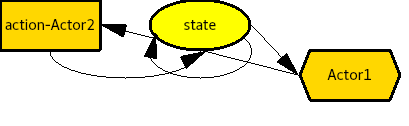
\includegraphics[width=0.4\textwidth]{/home/david/psychsim/psychsim/tools/simple.png}%
\caption{Simple influence diagram}%
\end{figure}

%
\begin{itemize}%
\item%
Rectangular nodes are possible actions for a particular agent (``Actor 1'', indicated by color) representing a potential behavior. They are labeled with a verb (``action'') and an optional object of the verb (``Actor2''). An action node has a binary value, indicating whether or not the action was chosen.%
\item%
Oval nodes are state variables. Their value is potentially a probability distribution over a domain of possible values. All true state variables will be certain (i.e., 100\% probability for a single value), but agents' perceptions of the true state will often be uncertain.%
\item%
Hexagonal nodes are utility or reward nodes. They represent an expected value computation by the agent (``Actor1''). The node's value is a table with each row corresponding to a possible action choice and its expected utility.%
\item%
Links from action nodes to state nodes specify an effect that the action has on the value of the state. In the following specifications of these effects, a variable name followed by a ' will denote the value of the variable after the action is performed.%
\item%
Links from one state node to another specify an influence that the value of the first state node has on the effect of at least one action on the second state node.%
\item%
Links from a state node to an agent's utility node specify that the state node is an input to the expected value calculation performed by that agent. There is a real{-}valued weight from \$(0,1{]}\$ on each link specifying the priority of that variable's influence on that agent's reward calculation (higher values mean higher priority).%
\item%
Links from utility nodes to action nodes indicate that the expected value calculation then determines whether or not that action is chosen. In the simulations described here, we use a strict maximization, so that the action choice is deterministic (i.e., the action with the highest expected value is performed, with ties broken by a pre{-}determined fixed order).%
\item%
Therefore, in the above simple ground truth, whether or not ``Actor1'' chooses to do ``action'' to ``Actor2'' influences the subsequent value of the variable ``state'' (link from rectangle to oval). The subsequent value of ``state'' also depends on its prior value (link from oval to itself). ``Actor1'''s expected value of doing ``action'' to ``Actor2'' is a function of the value of ``state'' (link from oval to hexagon), and this expected value influences whether or not ``Actor1'' chooses to do so (link from hexagon to rectangle).%
\end{itemize}%
Any real values (e.g., initial values of variables, conditional probability table values, reward weights) will be drawn from either a set \{0, 0.5, 1\} or \{0, 0.2, 0.4, 0.6, 0.8, 1\}, depending on the appropriate granularity needed.

%
\section{State}%
\label{sec:State}%
\subsection{Actor's age}%
\label{subsec:Actor's age}%
\begin{description}%
\item[Type:]%
Integer%
\end{description}%
\begin{flushleft}%
\verb|psychsim/domains/groundtruth/simulation/actor.py:80|%
\end{flushleft}

%
\subsection{Actor's alive}%
\label{subsec:Actor's alive}%
\begin{description}%
\item[Type:]%
Boolean%
\end{description}%
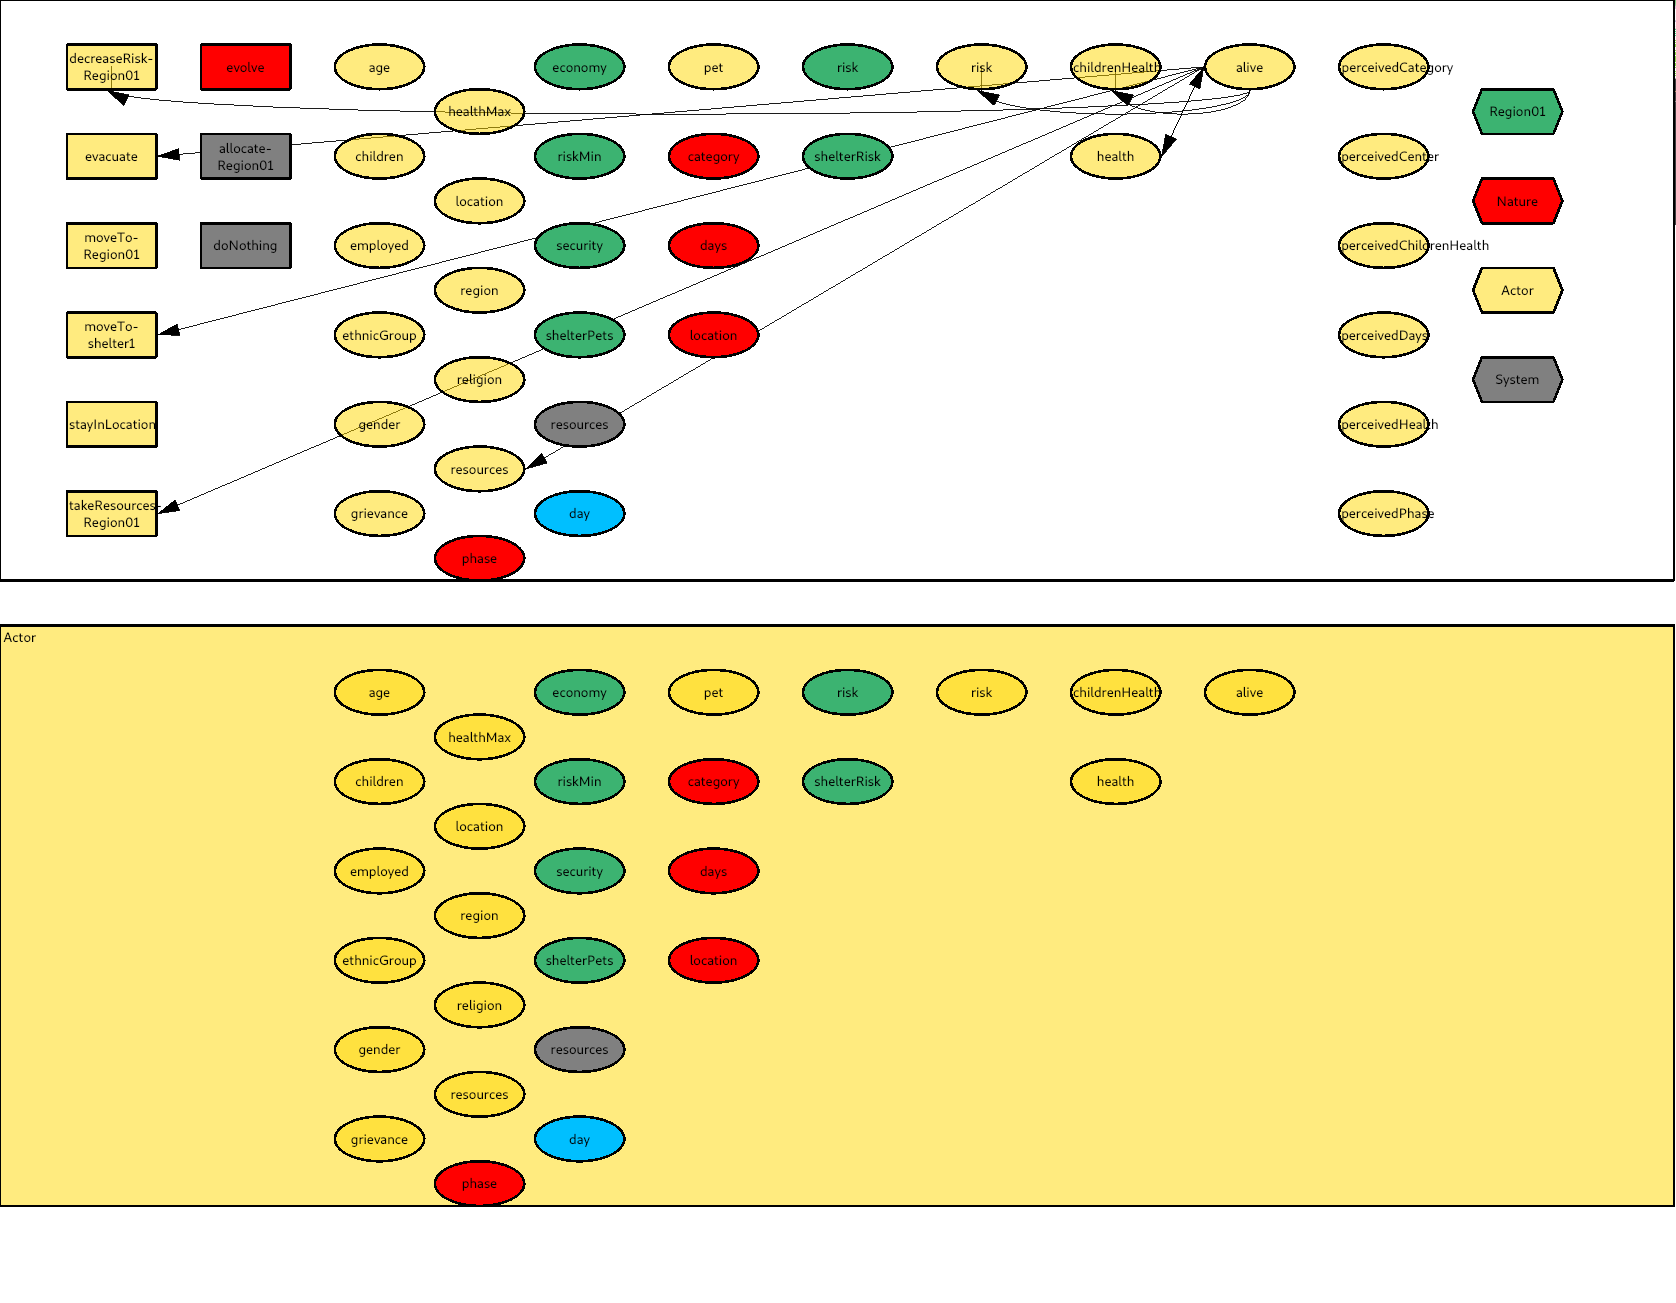
\includegraphics[width=\textwidth]{images/aliveOfActor.png}%
\begin{flushleft}%
\verb|psychsim/domains/groundtruth/simulation/actor.py:205|%
\end{flushleft}%
\subsubsection{Default change in Actor's alive}%
\label{ssubsec:Default change in Actor's alive}%
\begin{flushleft}%
\verb|psychsim/domains/groundtruth/simulation/actor.py:491|%
\linebreak%
IF %
\textbf{Actor's alive}%
\linebreak%
\hspace*{2em}%
THEN %
: %
IF %
$\mbox{\textbf{Actor's health}} '$%
$>$%
0.01%
\linebreak%
\hspace*{4em}%
THEN %
: %
$\mbox{\textbf{Actor's alive}} '$%
$\leftarrow$%
\textbf{true}%
\linebreak%
\hspace*{4em}%
ELSE %
: %
$\mbox{\textbf{Actor's alive}} '$%
$\leftarrow$%
\textbf{false}%
\linebreak%
\hspace*{2em}%
ELSE %
: %
$\mbox{\textbf{Actor's alive}} '$%
$\leftarrow$%
\textbf{Actor's alive}%
\end{flushleft}

%
\subsection{Actor's children}%
\label{subsec:Actor's children}%
Number of children%
\begin{description}%
\item[Type:]%
Real%
\end{description}%
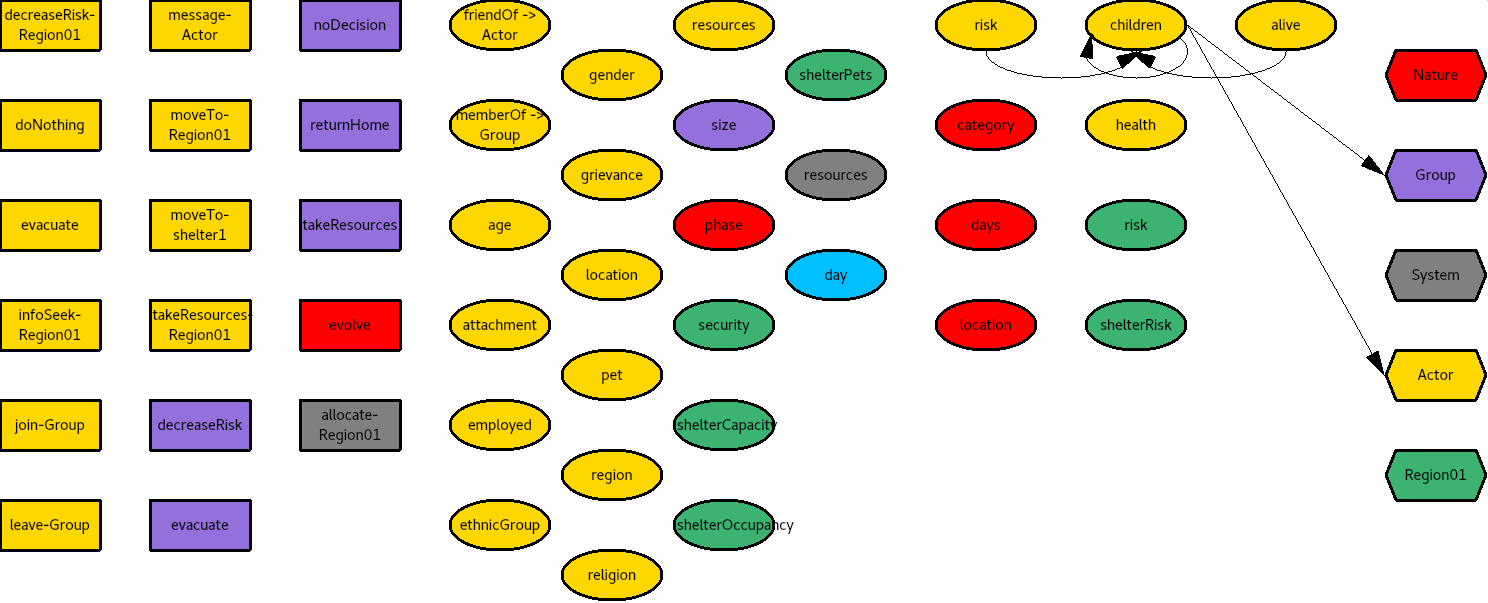
\includegraphics[width=\textwidth]{images/childrenOfActor.png}%
\begin{flushleft}%
\verb|psychsim/domains/groundtruth/simulation/actor.py:89|%
\end{flushleft}

%
\subsection{Actor's childrenHealth}%
\label{subsec:Actor's childrenHealth}%
Current level of children's physical wellbeing%
\begin{description}%
\item[Type:]%
Real%
\end{description}%
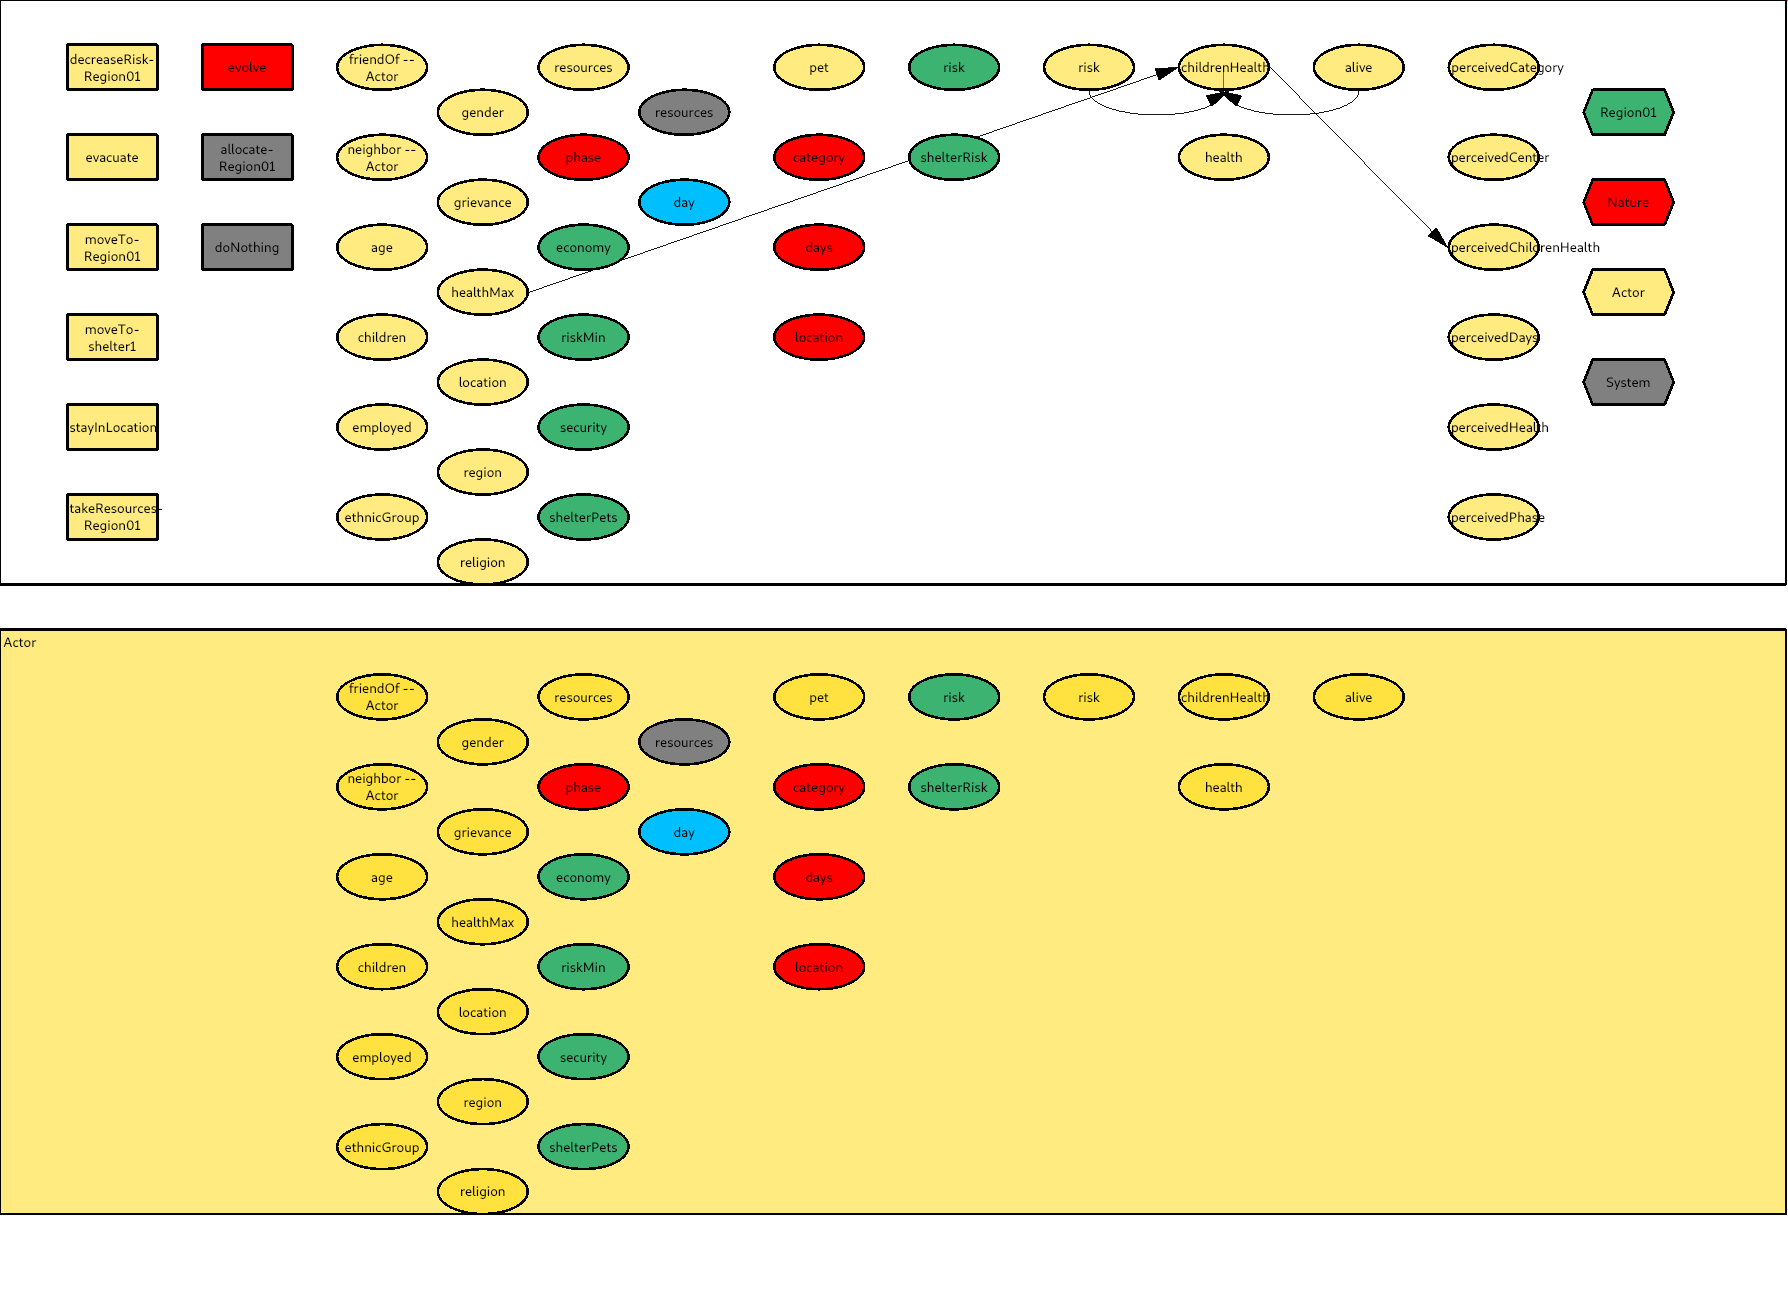
\includegraphics[width=\textwidth]{images/childrenHealthOfActor.png}%
\begin{flushleft}%
\verb|psychsim/domains/groundtruth/simulation/actor.py:230|%
\end{flushleft}%
\subsubsection{Effect of Actor on Actor's childrenHealth}%
\label{ssubsec:Effect of Actor on Actor's childrenHealth}%
\begin{flushleft}%
\verb|psychsim/domains/groundtruth/simulation/actor.py:480|%
\linebreak%
IF %
\textbf{Actor's alive}%
\linebreak%
\hspace*{2em}%
THEN %
: %
IF %
$\mbox{\textbf{Actor's risk}} '$%
$\in$%
\linebreak%
\hspace*{4em}%
{[}0,0.2{]}%
: %
$\mbox{\textbf{Actor's childrenHealth}} '$%
$\leftarrow$%
60\%%
$\cdot$%
\textbf{Actor's childrenHealth}%
+%
40\%%
$\cdot$%
\textbf{Actor's healthMax}%
\linebreak%
\hspace*{4em}%
(0.2,0.4{]}%
: %
\linebreak%
\hspace*{6em}%
20\%%
: %
$\mbox{\textbf{Actor's childrenHealth}} '$%
$\leftarrow$%
60\%%
$\cdot$%
\textbf{Actor's childrenHealth}%
\linebreak%
\hspace*{6em}%
80\%%
: %
$\mbox{\textbf{Actor's childrenHealth}} '$%
$\leftarrow$%
60\%%
$\cdot$%
\textbf{Actor's childrenHealth}%
+%
40\%%
$\cdot$%
\textbf{Actor's healthMax}%
\linebreak%
\hspace*{4em}%
(0.4,0.6{]}%
: %
\linebreak%
\hspace*{6em}%
40\%%
: %
$\mbox{\textbf{Actor's childrenHealth}} '$%
$\leftarrow$%
60\%%
$\cdot$%
\textbf{Actor's childrenHealth}%
\linebreak%
\hspace*{6em}%
60\%%
: %
$\mbox{\textbf{Actor's childrenHealth}} '$%
$\leftarrow$%
60\%%
$\cdot$%
\textbf{Actor's childrenHealth}%
+%
40\%%
$\cdot$%
\textbf{Actor's healthMax}%
\linebreak%
\hspace*{4em}%
(0.6,0.8{]}%
: %
\linebreak%
\hspace*{6em}%
60\%%
: %
$\mbox{\textbf{Actor's childrenHealth}} '$%
$\leftarrow$%
60\%%
$\cdot$%
\textbf{Actor's childrenHealth}%
\linebreak%
\hspace*{6em}%
40\%%
: %
$\mbox{\textbf{Actor's childrenHealth}} '$%
$\leftarrow$%
60\%%
$\cdot$%
\textbf{Actor's childrenHealth}%
+%
40\%%
$\cdot$%
\textbf{Actor's healthMax}%
\linebreak%
\hspace*{4em}%
(0.8,1.0{]}%
: %
\linebreak%
\hspace*{6em}%
80\%%
: %
$\mbox{\textbf{Actor's childrenHealth}} '$%
$\leftarrow$%
60\%%
$\cdot$%
\textbf{Actor's childrenHealth}%
\linebreak%
\hspace*{6em}%
19\%%
: %
$\mbox{\textbf{Actor's childrenHealth}} '$%
$\leftarrow$%
60\%%
$\cdot$%
\textbf{Actor's childrenHealth}%
+%
40\%%
$\cdot$%
\textbf{Actor's healthMax}%
\linebreak%
\hspace*{4em}%
(1.0,1{]}%
: %
\linebreak%
\hspace*{6em}%
100\%%
: %
$\mbox{\textbf{Actor's childrenHealth}} '$%
$\leftarrow$%
60\%%
$\cdot$%
\textbf{Actor's childrenHealth}%
\linebreak%
\hspace*{6em}%
0\%%
: %
$\mbox{\textbf{Actor's childrenHealth}} '$%
$\leftarrow$%
60\%%
$\cdot$%
\textbf{Actor's childrenHealth}%
+%
40\%%
$\cdot$%
\textbf{Actor's healthMax}%
\linebreak%
\hspace*{2em}%
ELSE %
: %
$\mbox{\textbf{Actor's childrenHealth}} '$%
$\leftarrow$%
0.00%
\end{flushleft}

%
\subsection{Actor's employed}%
\label{subsec:Actor's employed}%
Has a full{-}time job%
\begin{description}%
\item[Type:]%
Boolean%
\end{description}%
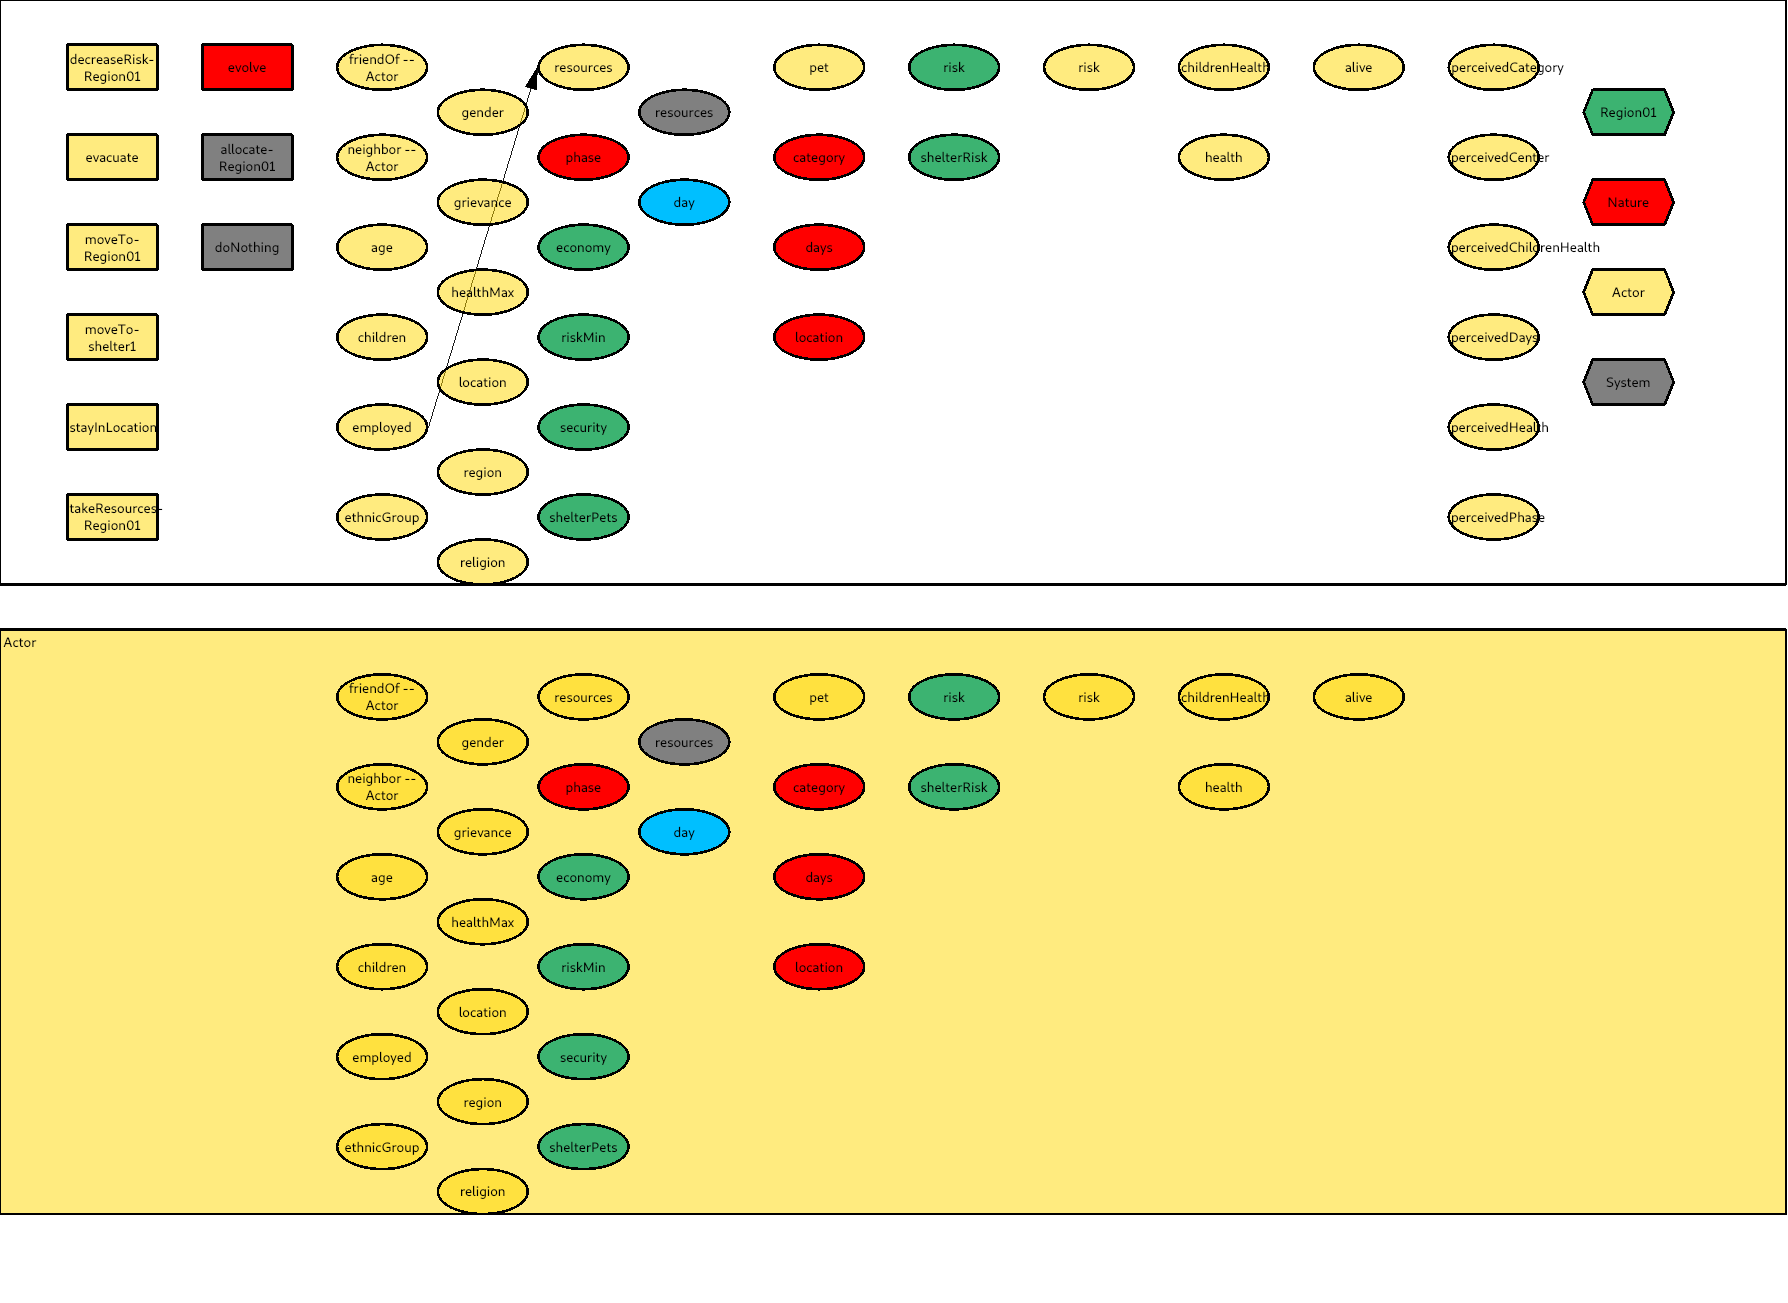
\includegraphics[width=\textwidth]{images/employedOfActor.png}%
\begin{flushleft}%
\verb|psychsim/domains/groundtruth/simulation/actor.py:97|%
\end{flushleft}

%
\subsection{Actor's ethnicGroup}%
\label{subsec:Actor's ethnicGroup}%
Ethnicity of actor%
\begin{description}%
\item[Type:]%
String%
\item[Values:]%
\textbf{majority}%
, %
\textbf{minority}%
\end{description}%
\begin{flushleft}%
\verb|psychsim/domains/groundtruth/simulation/actor.py:53|%
\end{flushleft}

%
\subsection{Actor's gender}%
\label{subsec:Actor's gender}%
\begin{description}%
\item[Type:]%
String%
\item[Values:]%
\textbf{female}%
, %
\textbf{male}%
\end{description}%
\begin{flushleft}%
\verb|psychsim/domains/groundtruth/simulation/actor.py:72|%
\end{flushleft}

%
\subsection{Actor's grievance}%
\label{subsec:Actor's grievance}%
Current level of grievance felt toward system%
\begin{description}%
\item[Type:]%
Real%
\end{description}%
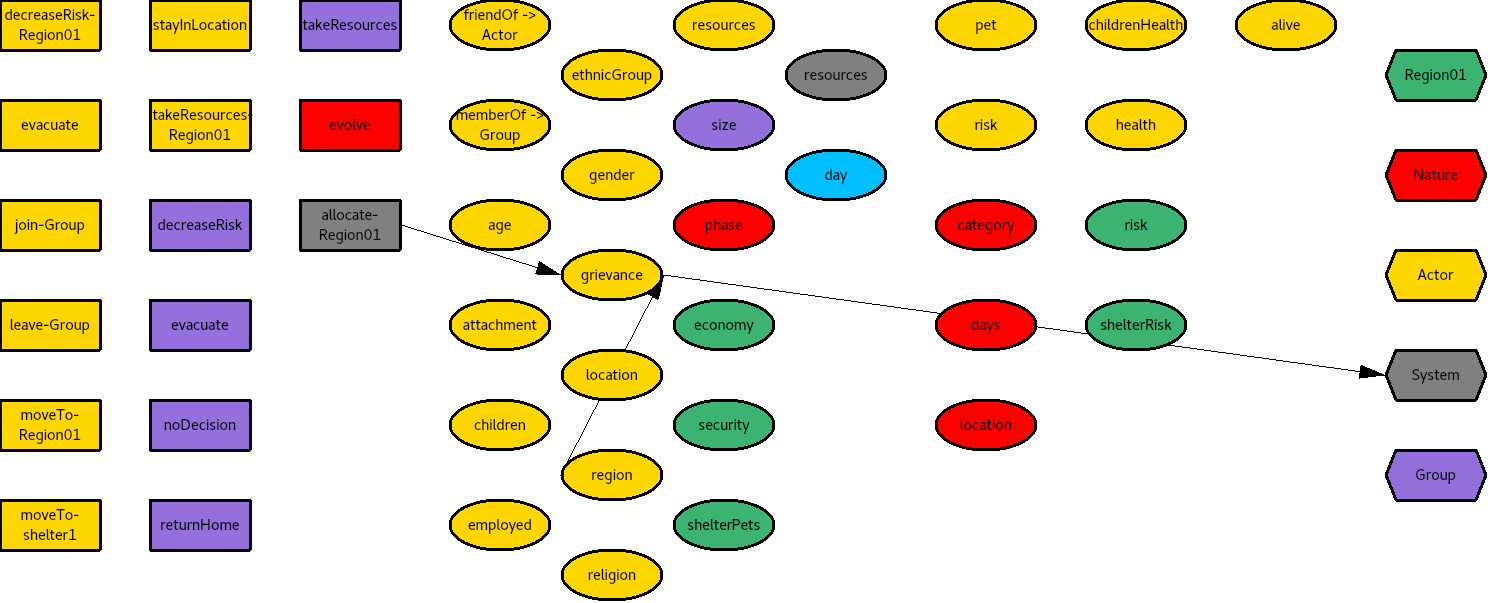
\includegraphics[width=\textwidth]{images/grievanceOfActor.png}%
\begin{flushleft}%
\verb|psychsim/domains/groundtruth/simulation/actor.py:266|%
\end{flushleft}%
\subsubsection{Effect of System{-}allocate{-}Region01 on Actor's grievance}%
\label{ssubsec:Effect of System{-}allocate{-}Region01 on Actor's grievance}%
\begin{flushleft}%
\verb|psychsim/domains/groundtruth/simulation/system.py:54|%
\linebreak%
IF %
\textbf{Actor's region}%
$=$%
\textbf{Region01}%
\linebreak%
\hspace*{2em}%
THEN %
: %
$\mbox{\textbf{Actor's grievance}} '$%
$\leftarrow$%
80\%%
$\cdot$%
\textbf{Actor's grievance}%
\linebreak%
\hspace*{2em}%
ELSE %
: %
$\mbox{\textbf{Actor's grievance}} '$%
$\leftarrow$%
80\%%
$\cdot$%
\textbf{Actor's grievance}%
+0.20%
\end{flushleft}

%
\subsection{Actor's health}%
\label{subsec:Actor's health}%
Current level of physical wellbeing%
\begin{description}%
\item[Type:]%
Real%
\end{description}%
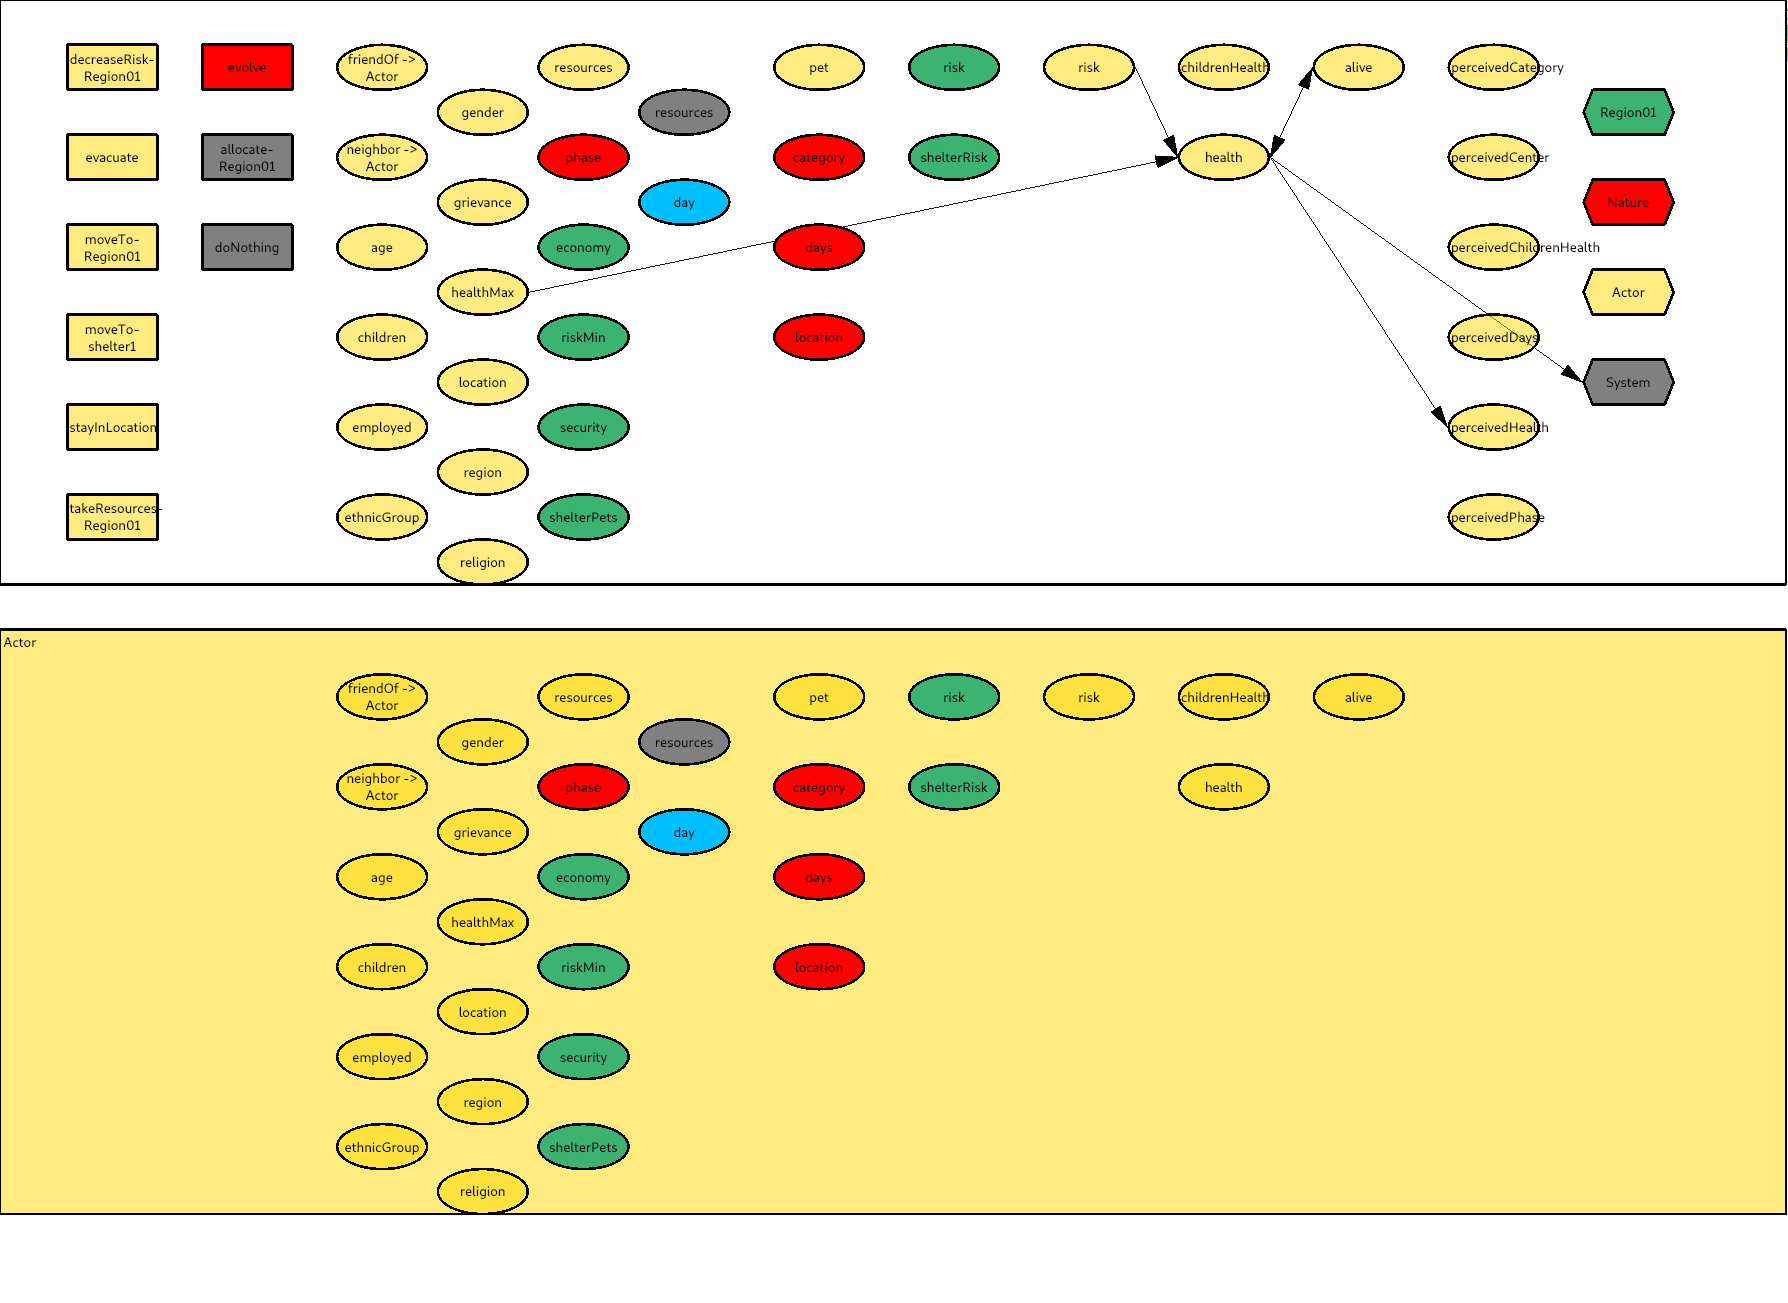
\includegraphics[width=\textwidth]{images/healthOfActor.png}%
\begin{flushleft}%
\verb|psychsim/domains/groundtruth/simulation/actor.py:209|%
\end{flushleft}%
\subsubsection{Effect of Actor on Actor's health}%
\label{ssubsec:Effect of Actor on Actor's health}%
\begin{flushleft}%
\verb|psychsim/domains/groundtruth/simulation/actor.py:464|%
\linebreak%
IF %
\textbf{Actor's alive}%
\linebreak%
\hspace*{2em}%
THEN %
: %
IF %
$\mbox{\textbf{Actor's risk}} '$%
$\in$%
\linebreak%
\hspace*{4em}%
{[}0,0.2{]}%
: %
$\mbox{\textbf{Actor's health}} '$%
$\leftarrow$%
60\%%
$\cdot$%
\textbf{Actor's health}%
+%
40\%%
$\cdot$%
\textbf{Actor's healthMax}%
\linebreak%
\hspace*{4em}%
(0.2,0.4{]}%
: %
\linebreak%
\hspace*{6em}%
20\%%
: %
$\mbox{\textbf{Actor's health}} '$%
$\leftarrow$%
60\%%
$\cdot$%
\textbf{Actor's health}%
\linebreak%
\hspace*{6em}%
80\%%
: %
$\mbox{\textbf{Actor's health}} '$%
$\leftarrow$%
60\%%
$\cdot$%
\textbf{Actor's health}%
+%
40\%%
$\cdot$%
\textbf{Actor's healthMax}%
\linebreak%
\hspace*{4em}%
(0.4,0.6{]}%
: %
\linebreak%
\hspace*{6em}%
40\%%
: %
$\mbox{\textbf{Actor's health}} '$%
$\leftarrow$%
60\%%
$\cdot$%
\textbf{Actor's health}%
\linebreak%
\hspace*{6em}%
60\%%
: %
$\mbox{\textbf{Actor's health}} '$%
$\leftarrow$%
60\%%
$\cdot$%
\textbf{Actor's health}%
+%
40\%%
$\cdot$%
\textbf{Actor's healthMax}%
\linebreak%
\hspace*{4em}%
(0.6,0.8{]}%
: %
\linebreak%
\hspace*{6em}%
60\%%
: %
$\mbox{\textbf{Actor's health}} '$%
$\leftarrow$%
60\%%
$\cdot$%
\textbf{Actor's health}%
\linebreak%
\hspace*{6em}%
40\%%
: %
$\mbox{\textbf{Actor's health}} '$%
$\leftarrow$%
60\%%
$\cdot$%
\textbf{Actor's health}%
+%
40\%%
$\cdot$%
\textbf{Actor's healthMax}%
\linebreak%
\hspace*{4em}%
(0.8,1.0{]}%
: %
\linebreak%
\hspace*{6em}%
80\%%
: %
$\mbox{\textbf{Actor's health}} '$%
$\leftarrow$%
60\%%
$\cdot$%
\textbf{Actor's health}%
\linebreak%
\hspace*{6em}%
19\%%
: %
$\mbox{\textbf{Actor's health}} '$%
$\leftarrow$%
60\%%
$\cdot$%
\textbf{Actor's health}%
+%
40\%%
$\cdot$%
\textbf{Actor's healthMax}%
\linebreak%
\hspace*{4em}%
(1.0,1{]}%
: %
\linebreak%
\hspace*{6em}%
100\%%
: %
$\mbox{\textbf{Actor's health}} '$%
$\leftarrow$%
60\%%
$\cdot$%
\textbf{Actor's health}%
\linebreak%
\hspace*{6em}%
0\%%
: %
$\mbox{\textbf{Actor's health}} '$%
$\leftarrow$%
60\%%
$\cdot$%
\textbf{Actor's health}%
+%
40\%%
$\cdot$%
\textbf{Actor's healthMax}%
\linebreak%
\hspace*{2em}%
ELSE %
: %
$\mbox{\textbf{Actor's health}} '$%
$\leftarrow$%
0.00%
\end{flushleft}

%
\subsection{Actor's healthMax}%
\label{subsec:Actor's healthMax}%
Maximum level of physical wellbeing%
\begin{description}%
\item[Type:]%
Real%
\end{description}%
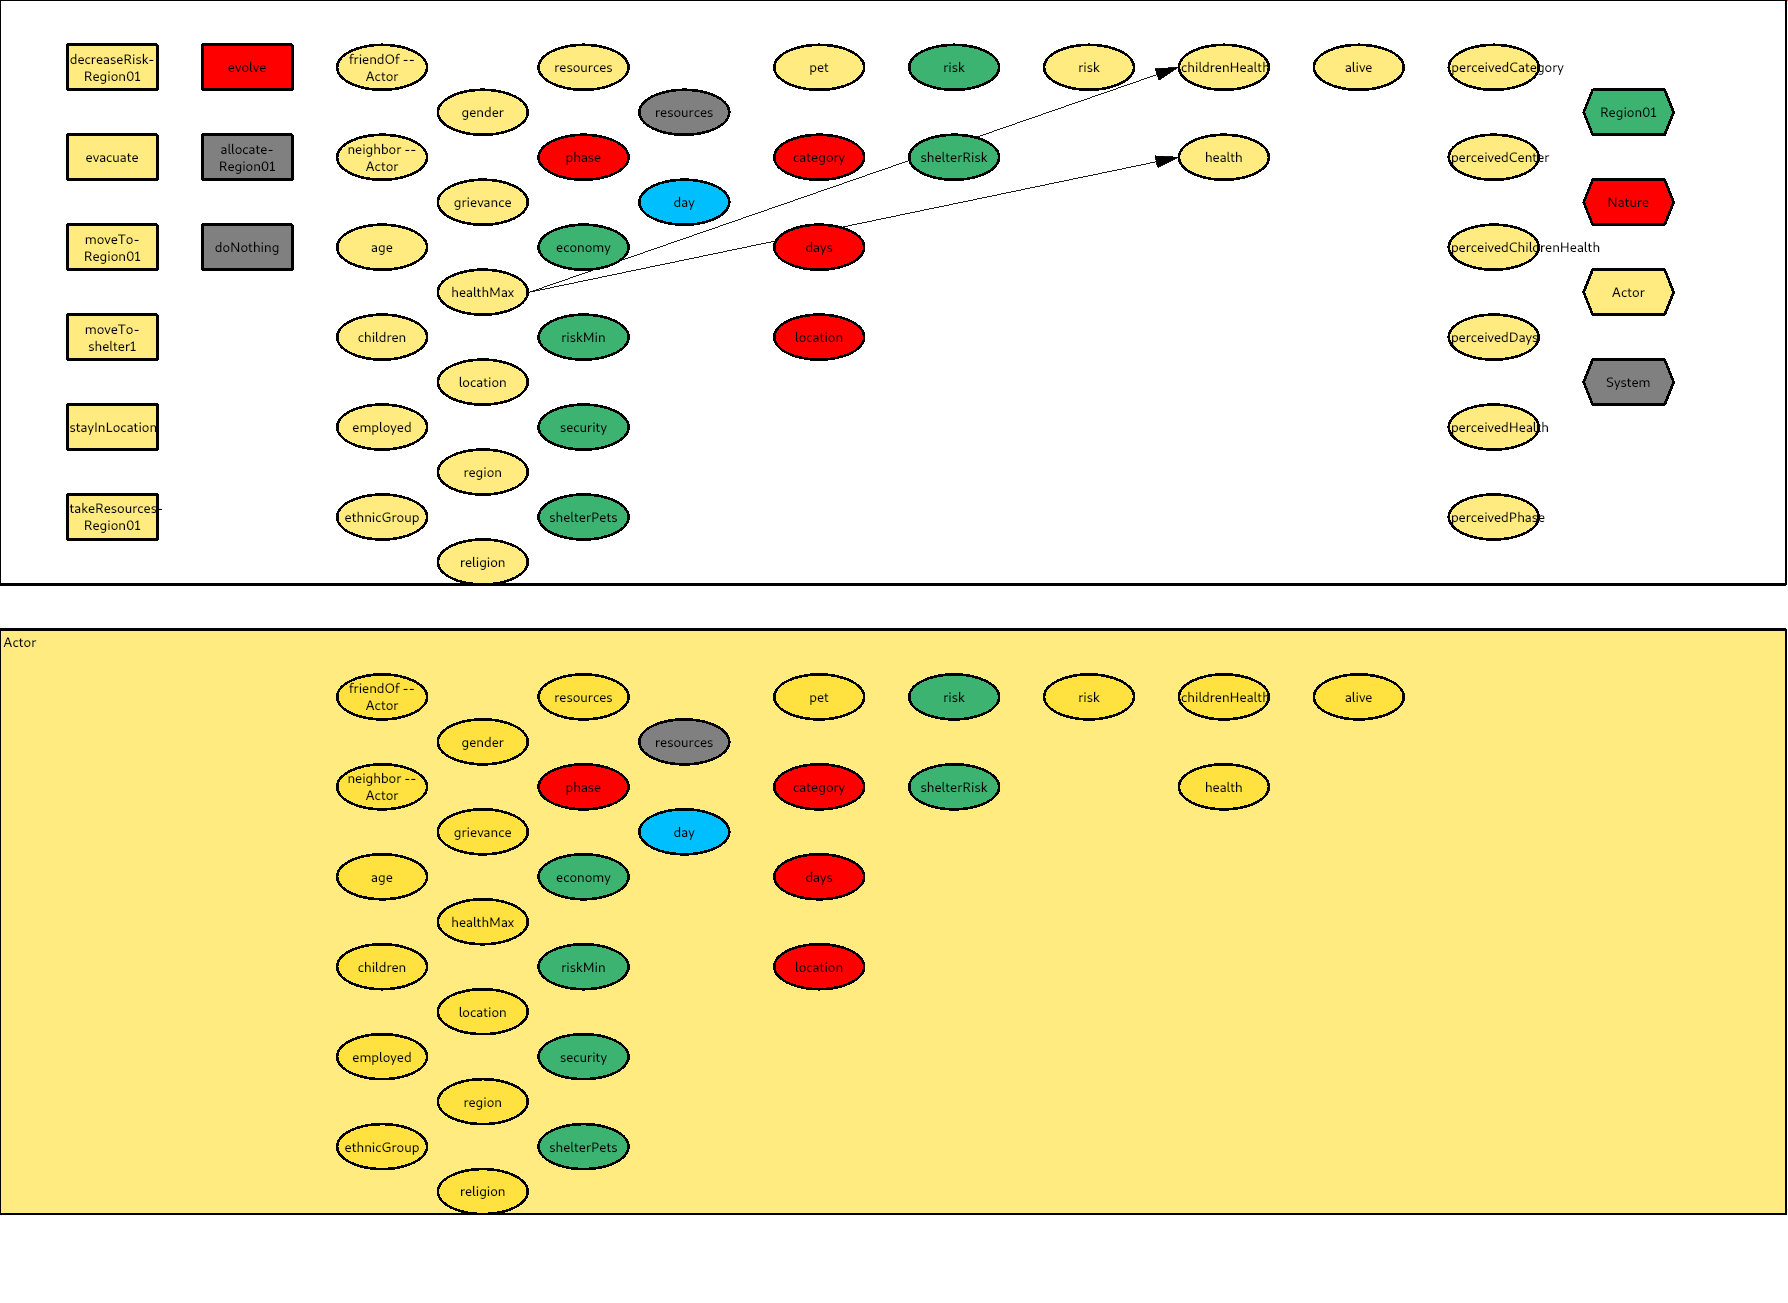
\includegraphics[width=\textwidth]{images/healthMaxOfActor.png}%
\begin{flushleft}%
\verb|psychsim/domains/groundtruth/simulation/actor.py:224|%
\end{flushleft}

%
\subsection{Actor's location}%
\label{subsec:Actor's location}%
Current location%
\begin{description}%
\item[Type:]%
String%
\item[Values:]%
\textbf{Region01}%
, %
\textbf{evacuated}%
, %
\textbf{shelter1}%
\end{description}%
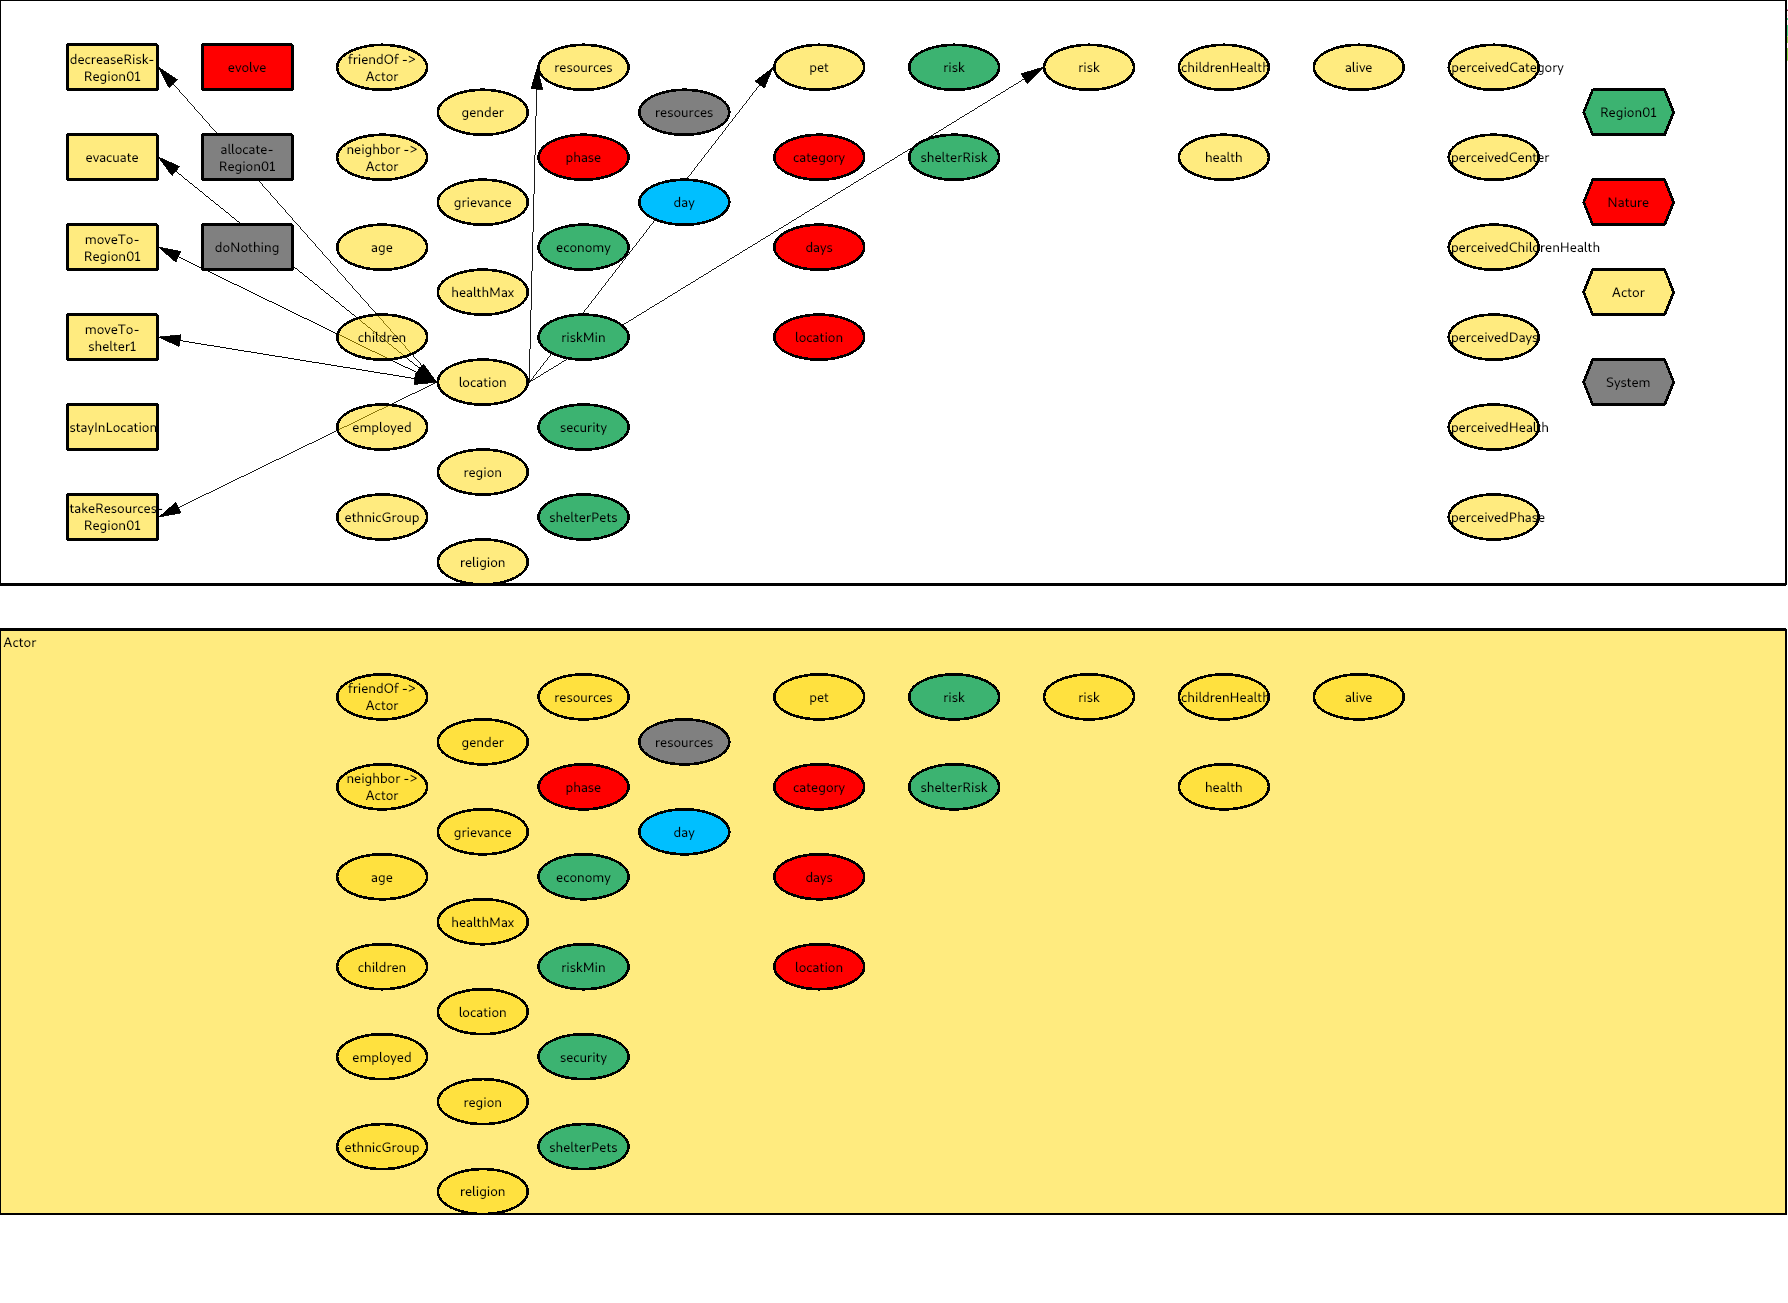
\includegraphics[width=\textwidth]{images/locationOfActor.png}%
\begin{flushleft}%
\verb|psychsim/domains/groundtruth/simulation/actor.py:202|%
\end{flushleft}%
\subsubsection{Effect of Actor{-}evacuate on Actor's location}%
\label{ssubsec:Effect of Actor{-}evacuate on Actor's location}%
\begin{flushleft}%
\verb|psychsim/domains/groundtruth/simulation/actor.py:420|%
\linebreak%
$\mbox{\textbf{Actor's location}} '$%
$\leftarrow$%
\textbf{evacuated}%
\end{flushleft}

%
\subsubsection{Effect of Actor{-}moveTo{-}Region01 on Actor's location}%
\label{ssubsec:Effect of Actor{-}moveTo{-}Region01 on Actor's location}%
\begin{flushleft}%
\verb|psychsim/domains/groundtruth/simulation/actor.py:427|%
\linebreak%
$\mbox{\textbf{Actor's location}} '$%
$\leftarrow$%
\textbf{Region01}%
\end{flushleft}

%
\subsubsection{Effect of Actor{-}moveTo{-}shelter1 on Actor's location}%
\label{ssubsec:Effect of Actor{-}moveTo{-}shelter1 on Actor's location}%
\begin{flushleft}%
\verb|psychsim/domains/groundtruth/simulation/actor.py:417|%
\linebreak%
$\mbox{\textbf{Actor's location}} '$%
$\leftarrow$%
\textbf{shelter1}%
\end{flushleft}

%
\subsection{Actor's perceivedCategory}%
\label{subsec:Actor's perceivedCategory}%
Perception of Nature's category%
\begin{description}%
\item[Type:]%
Integer%
\end{description}%
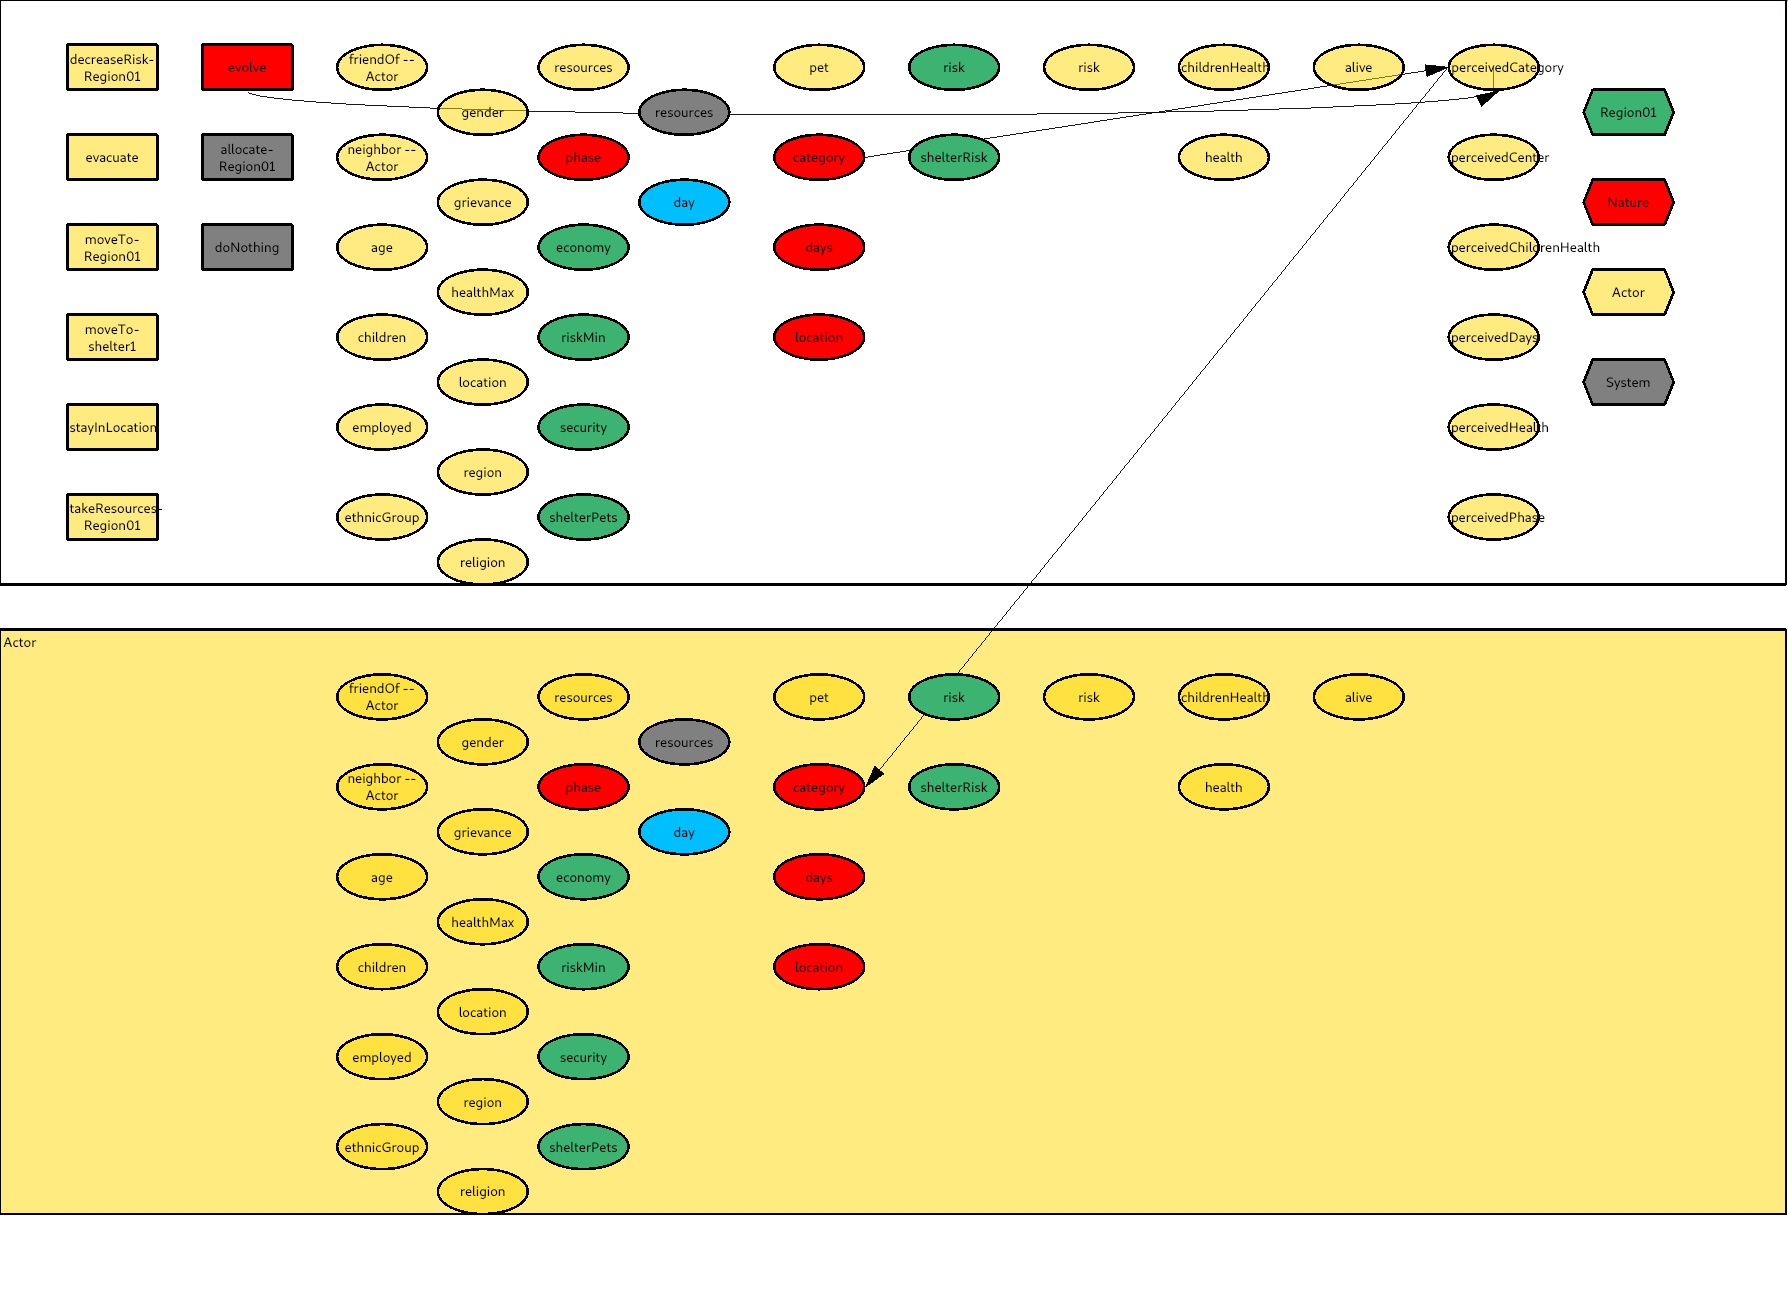
\includegraphics[width=\textwidth]{images/perceivedCategoryOfActor.png}%
\begin{flushleft}%
\verb|psychsim/domains/groundtruth/simulation/actor.py:685|%
\end{flushleft}%
\subsubsection{Observation function of Actor's perceivedCategory when Nature{-}evolve}%
\label{ssubsec:Observation function of Actor's perceivedCategory when Nature{-}evolve}%
\begin{flushleft}%
IF %
\textbf{Nature's category}%
$\in$%
\{0,5\}%
\linebreak%
\hspace*{2em}%
THEN %
: %
$\mbox{\textbf{Actor's perceivedCategory}} '$%
$\leftarrow$%
\textbf{Nature's category}%
\linebreak%
\hspace*{2em}%
ELSE %
: %
\linebreak%
\hspace*{4em}%
80\%%
: %
$\mbox{\textbf{Actor's perceivedCategory}} '$%
$\leftarrow$%
\textbf{Nature's category}%
\linebreak%
\hspace*{4em}%
19\%%
: %
$\mbox{\textbf{Actor's perceivedCategory}} '$%
$\leftarrow$%
\textbf{Nature's category}%
+1%
\end{flushleft}

%
\subsubsection{Default observation of Actor's perceivedCategory}%
\label{ssubsec:Default observation of Actor's perceivedCategory}%
\begin{flushleft}%
$\mbox{\textbf{Actor's perceivedCategory}} '$%
$\leftarrow$%
0%
\end{flushleft}

%
\subsection{Actor's perceivedCenter}%
\label{subsec:Actor's perceivedCenter}%
Perception of Nature's location%
\begin{description}%
\item[Type:]%
String%
\item[Values:]%
\textbf{Region01}%
, %
\textbf{none}%
\end{description}%
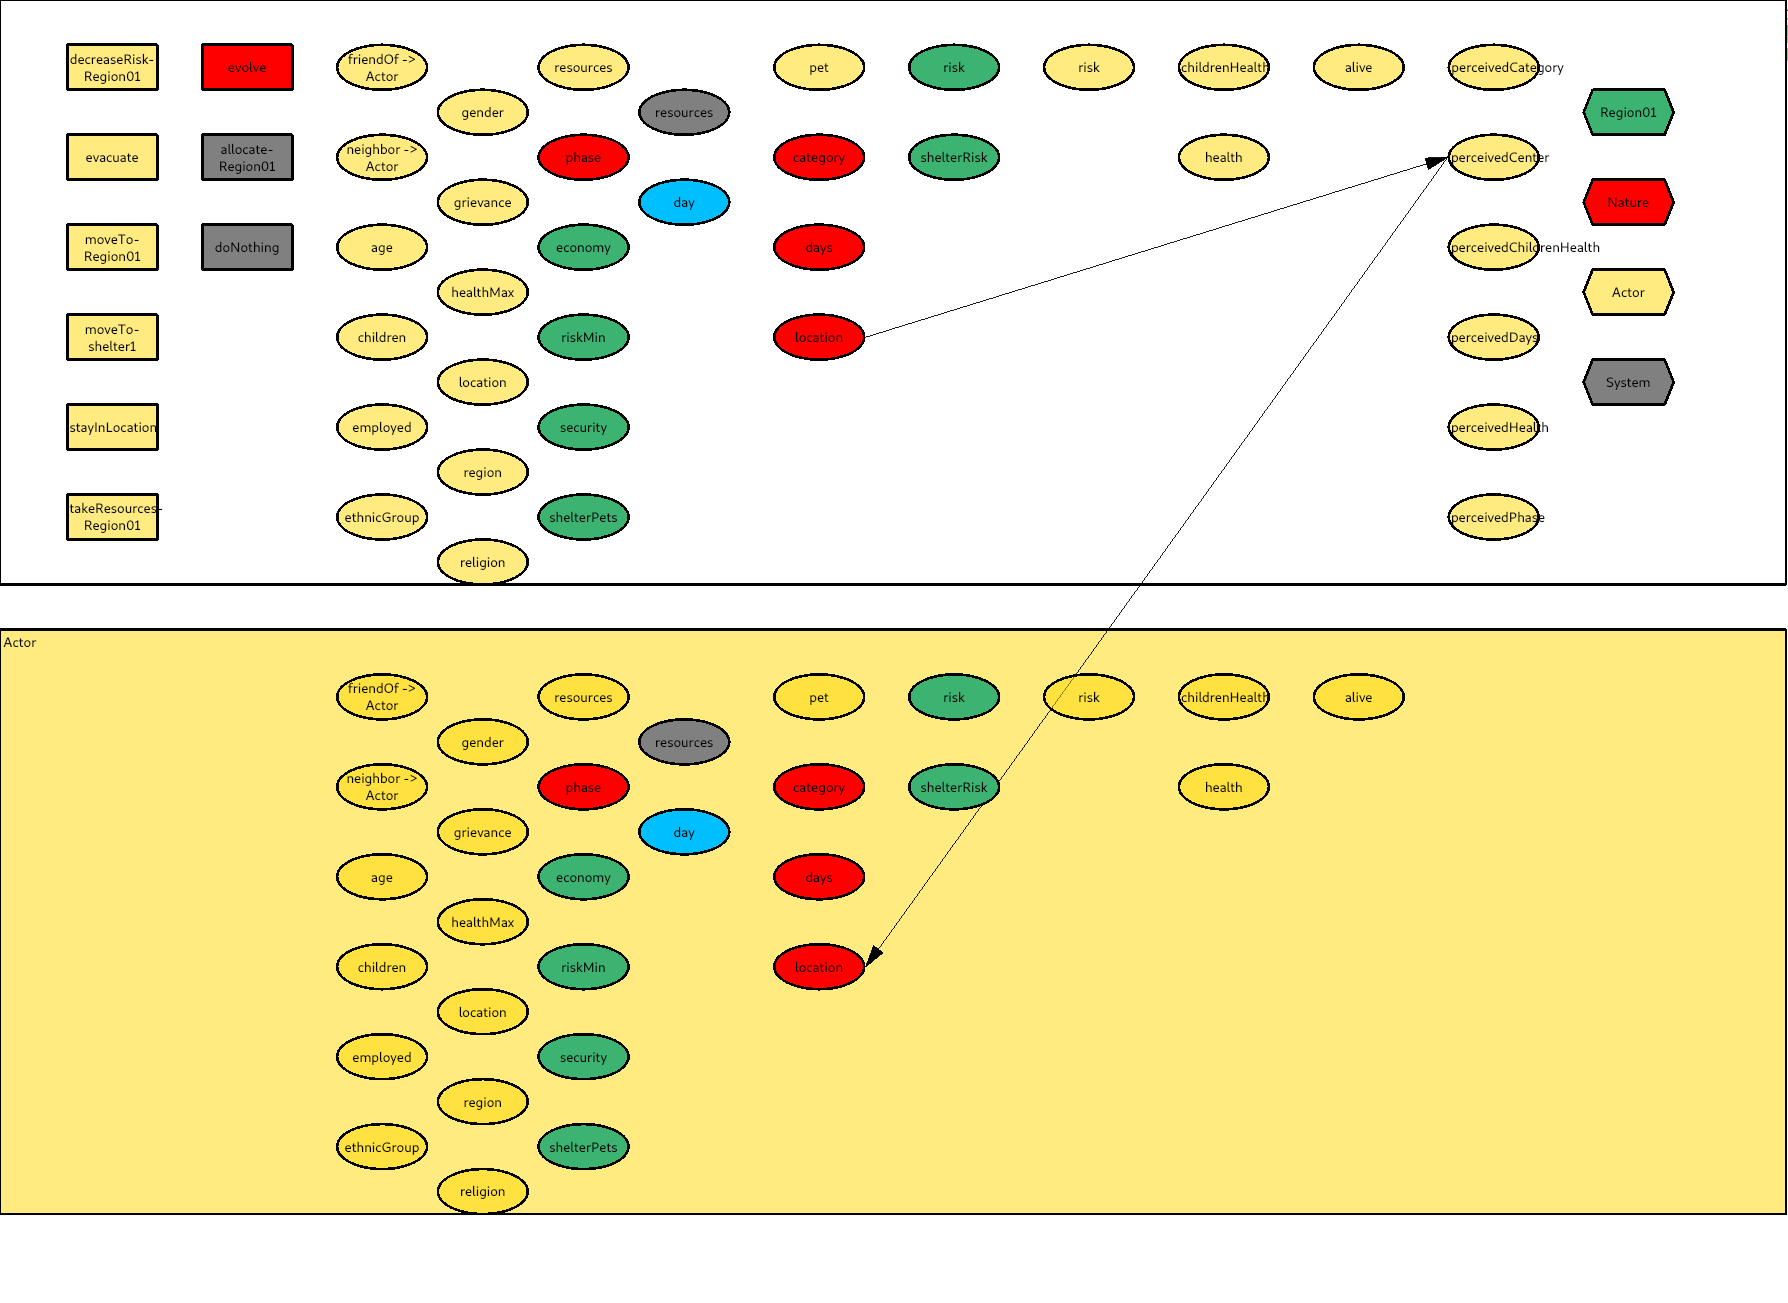
\includegraphics[width=\textwidth]{images/perceivedCenterOfActor.png}%
\begin{flushleft}%
\verb|psychsim/domains/groundtruth/simulation/actor.py:679|%
\end{flushleft}%
\subsubsection{Default observation of Actor's perceivedCenter}%
\label{ssubsec:Default observation of Actor's perceivedCenter}%
\begin{flushleft}%
$\mbox{\textbf{Actor's perceivedCenter}} '$%
$\leftarrow$%
\textbf{Nature's location}%
\end{flushleft}

%
\subsection{Actor's perceivedChildrenHealth}%
\label{subsec:Actor's perceivedChildrenHealth}%
Perception of Actor's childrenHealth%
\begin{description}%
\item[Type:]%
Real%
\end{description}%
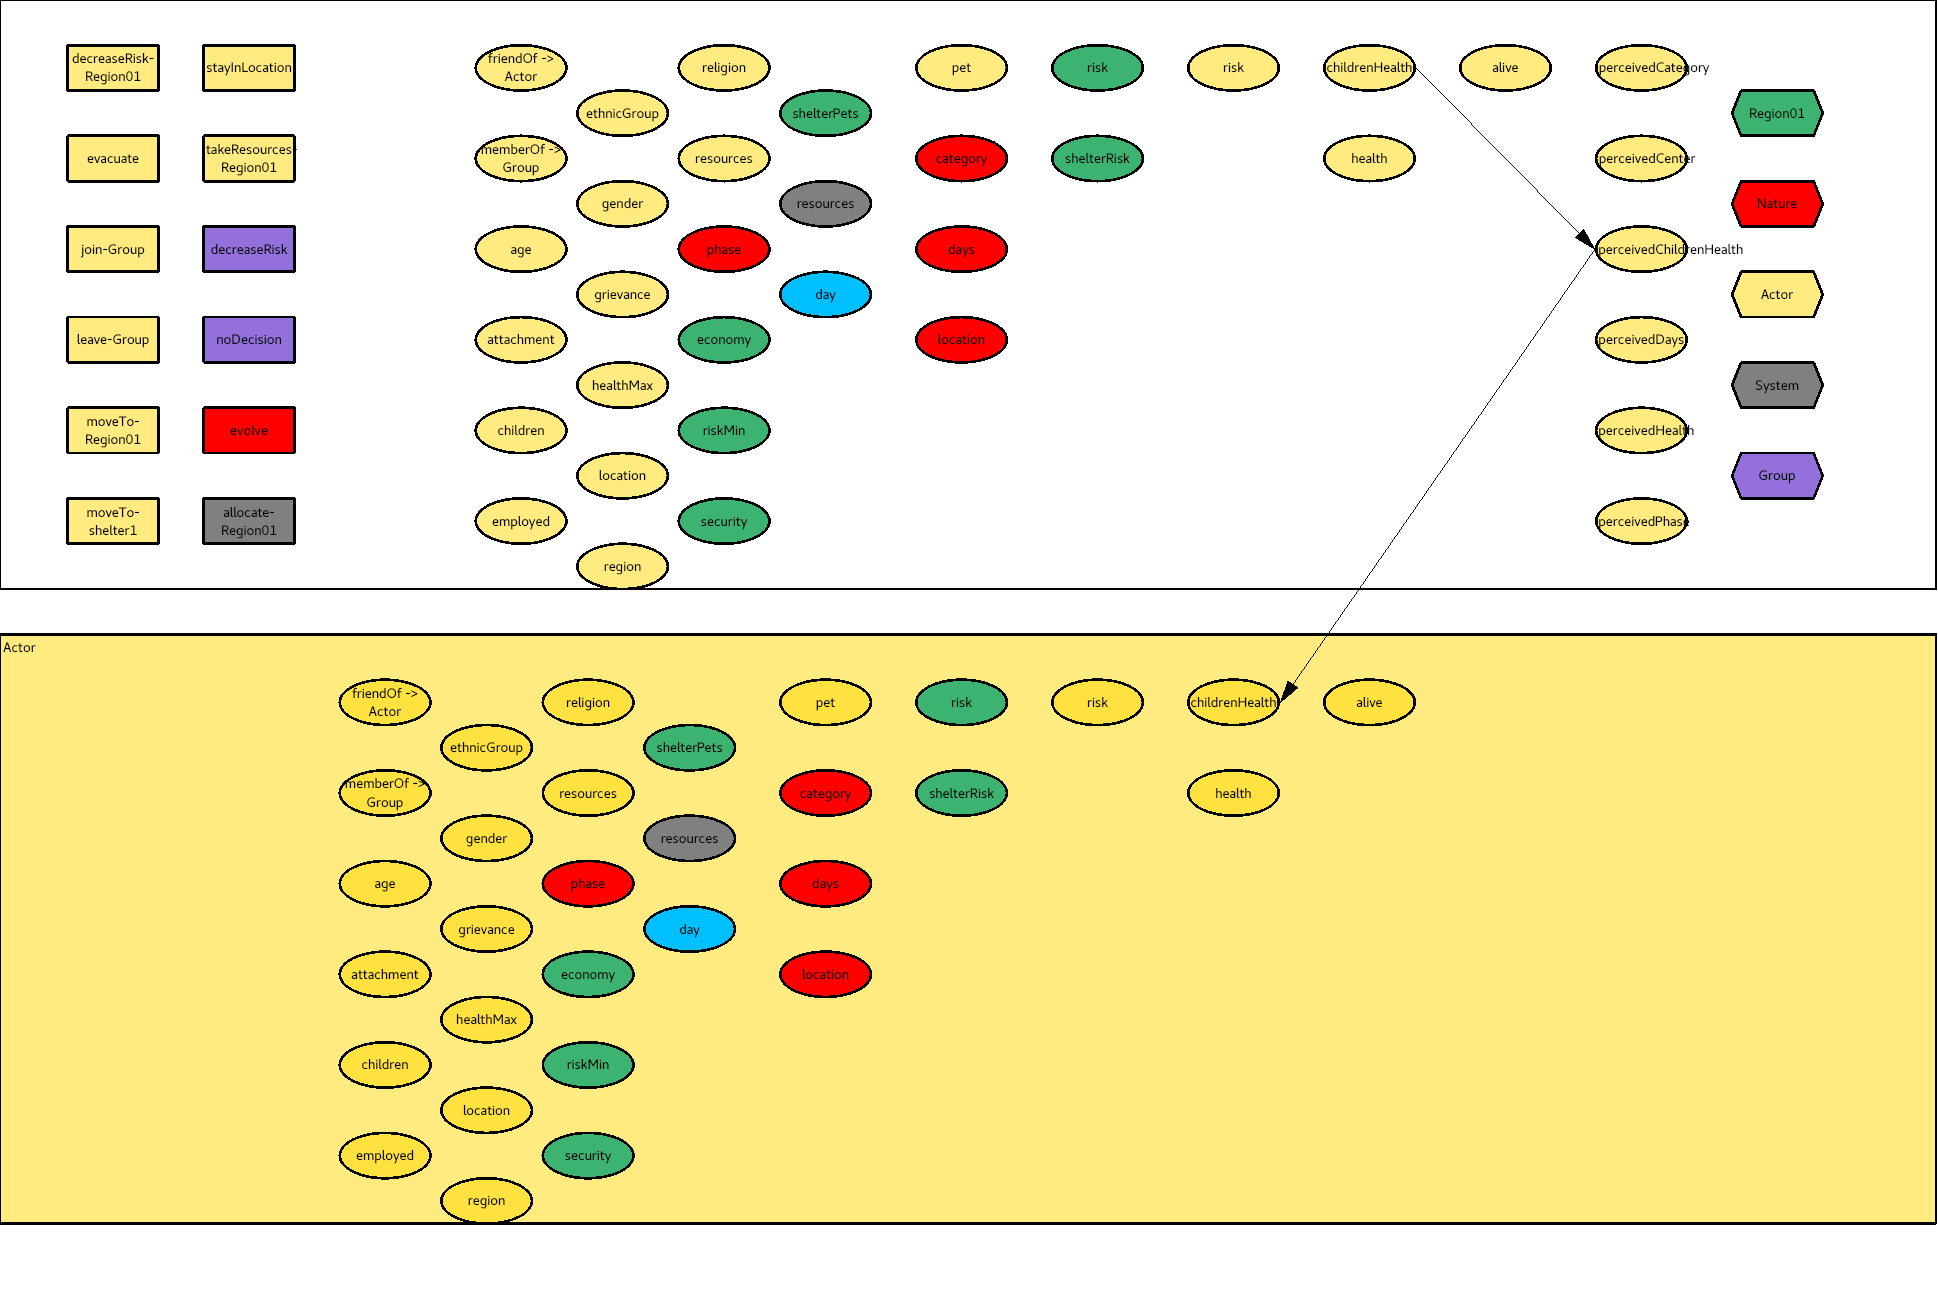
\includegraphics[width=\textwidth]{images/perceivedChildrenHealthOfActor.png}%
\begin{flushleft}%
\verb|psychsim/domains/groundtruth/simulation/actor.py:718|%
\end{flushleft}%
\subsubsection{Default observation of Actor's perceivedChildrenHealth}%
\label{ssubsec:Default observation of Actor's perceivedChildrenHealth}%
\begin{flushleft}%
$\mbox{\textbf{Actor's perceivedChildrenHealth}} '$%
$\leftarrow$%
\textbf{Actor's childrenHealth}%
\end{flushleft}

%
\subsection{Actor's perceivedDays}%
\label{subsec:Actor's perceivedDays}%
Perception of Nature's days%
\begin{description}%
\item[Type:]%
Integer%
\end{description}%
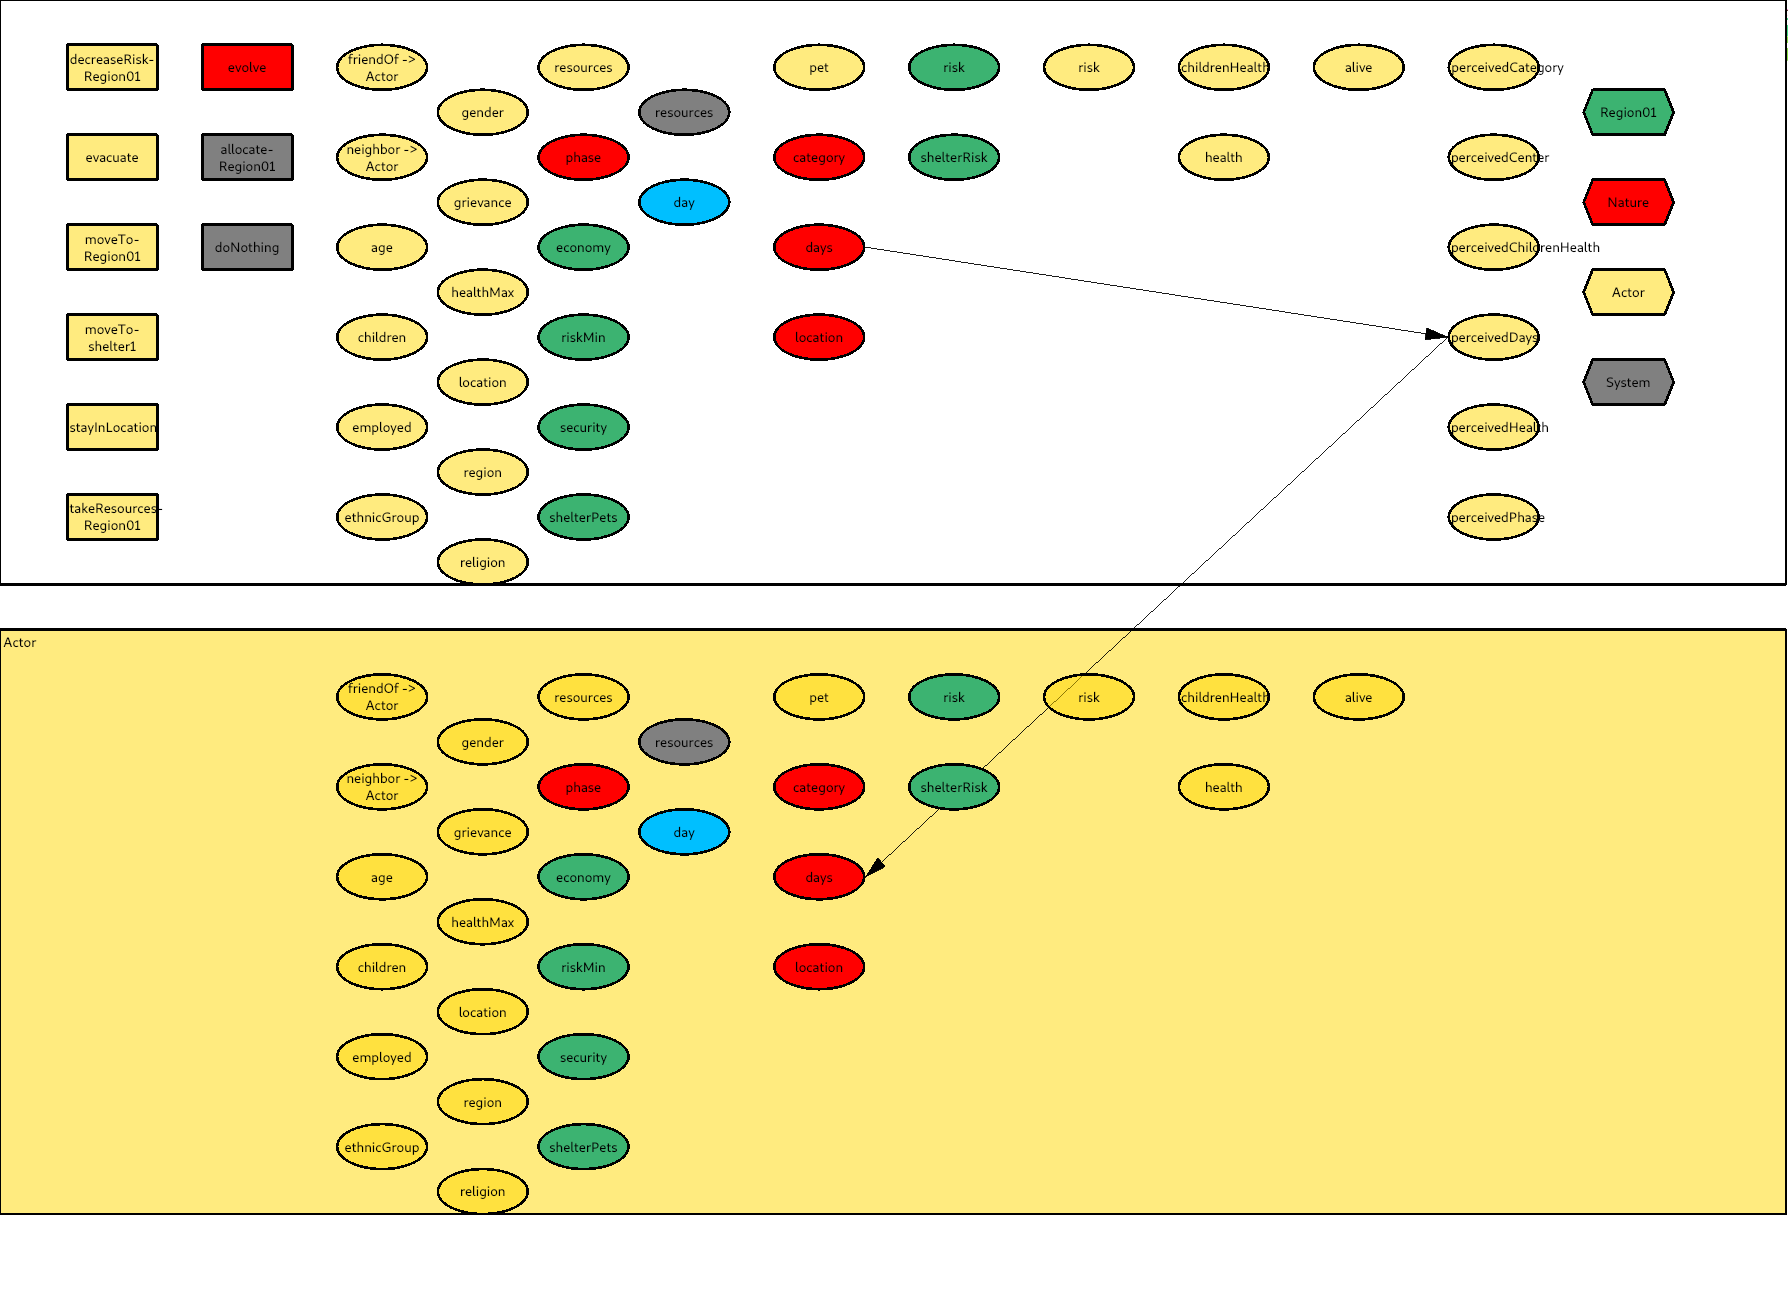
\includegraphics[width=\textwidth]{images/perceivedDaysOfActor.png}%
\begin{flushleft}%
\verb|psychsim/domains/groundtruth/simulation/actor.py:673|%
\end{flushleft}%
\subsubsection{Default observation of Actor's perceivedDays}%
\label{ssubsec:Default observation of Actor's perceivedDays}%
\begin{flushleft}%
$\mbox{\textbf{Actor's perceivedDays}} '$%
$\leftarrow$%
\textbf{Nature's days}%
\end{flushleft}

%
\subsection{Actor's perceivedHealth}%
\label{subsec:Actor's perceivedHealth}%
Perception of Actor's health%
\begin{description}%
\item[Type:]%
Real%
\end{description}%
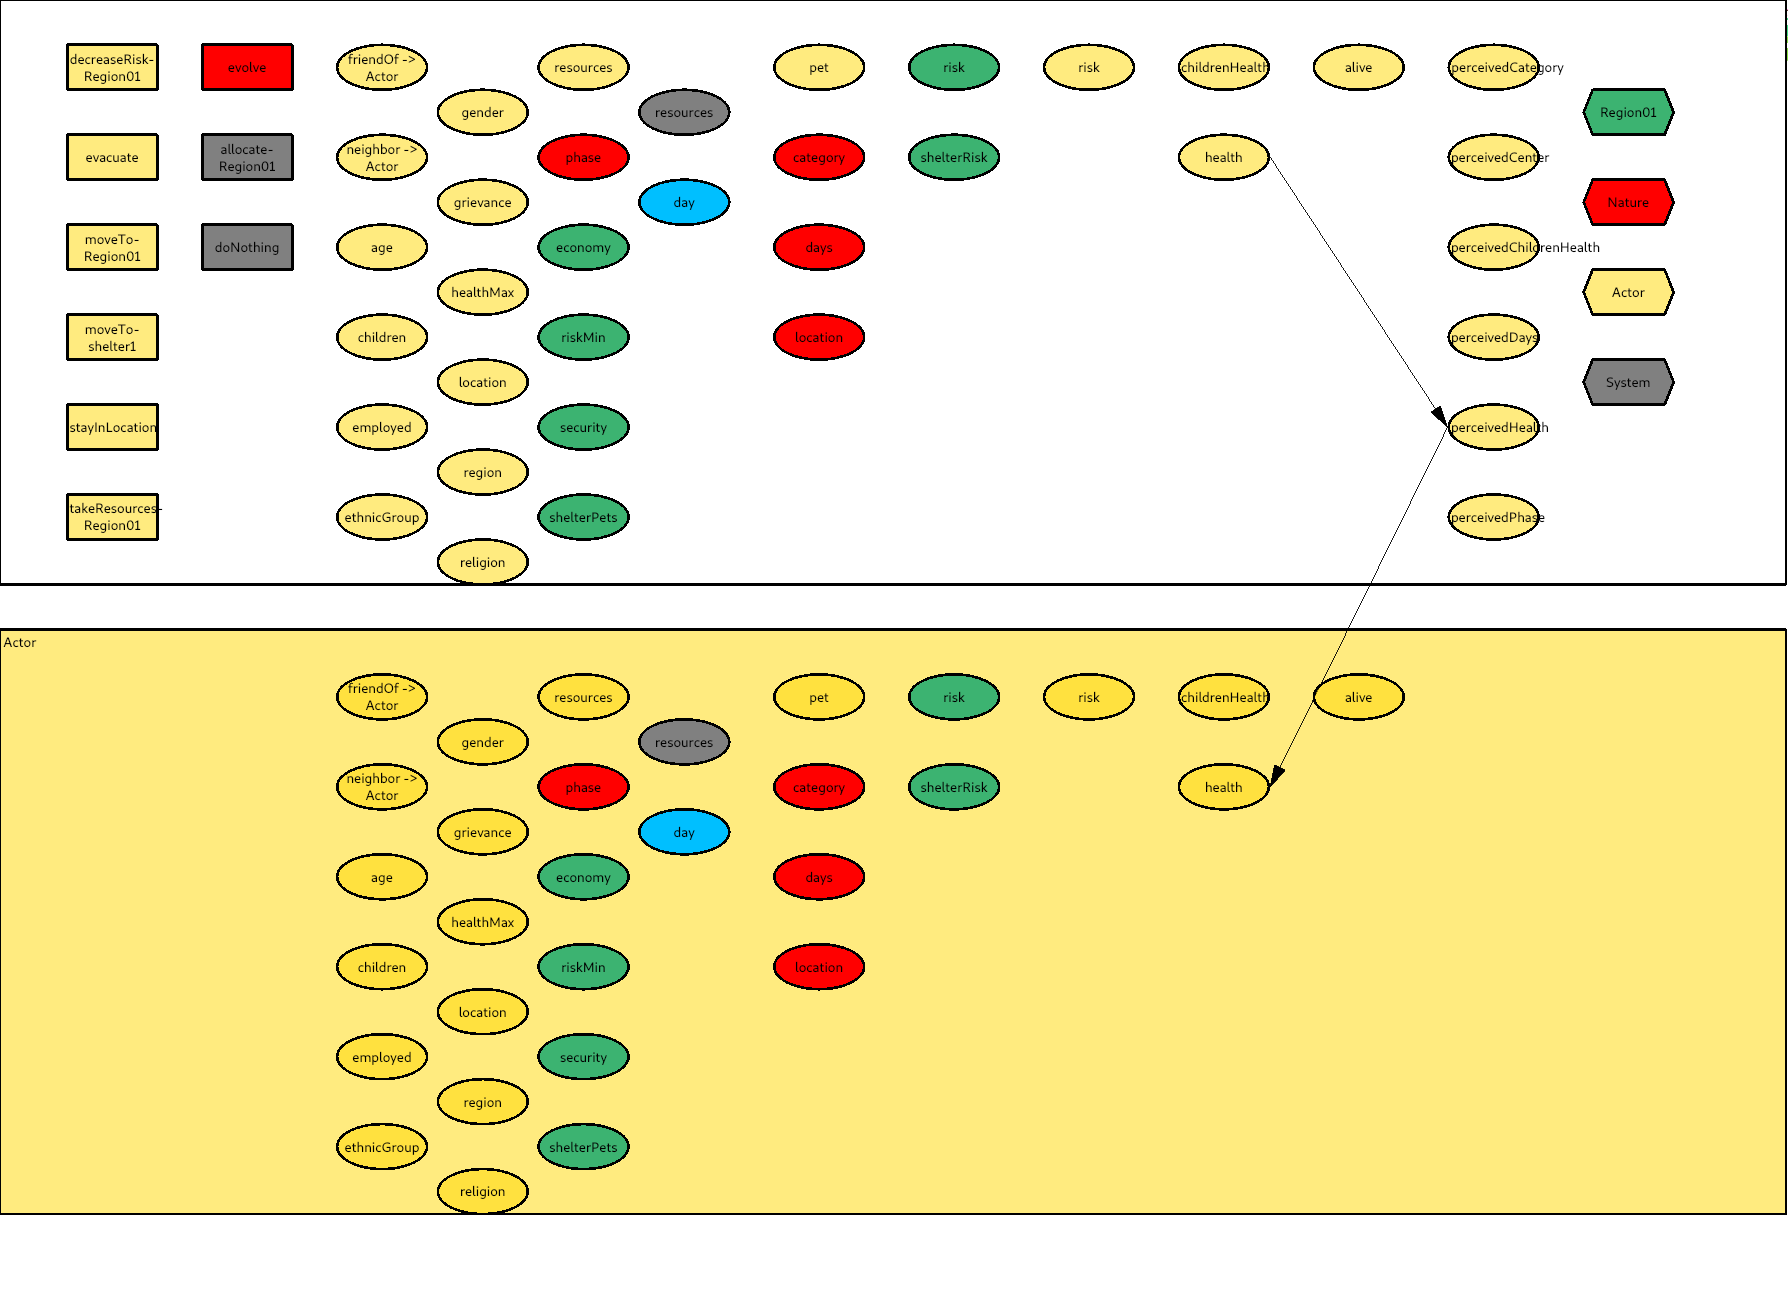
\includegraphics[width=\textwidth]{images/perceivedHealthOfActor.png}%
\begin{flushleft}%
\verb|psychsim/domains/groundtruth/simulation/actor.py:712|%
\end{flushleft}%
\subsubsection{Default observation of Actor's perceivedHealth}%
\label{ssubsec:Default observation of Actor's perceivedHealth}%
\begin{flushleft}%
$\mbox{\textbf{Actor's perceivedHealth}} '$%
$\leftarrow$%
\textbf{Actor's health}%
\end{flushleft}

%
\subsection{Actor's perceivedPhase}%
\label{subsec:Actor's perceivedPhase}%
Perception of Nature's phase%
\begin{description}%
\item[Type:]%
String%
\item[Values:]%
\textbf{active}%
, %
\textbf{approaching}%
, %
\textbf{none}%
\end{description}%
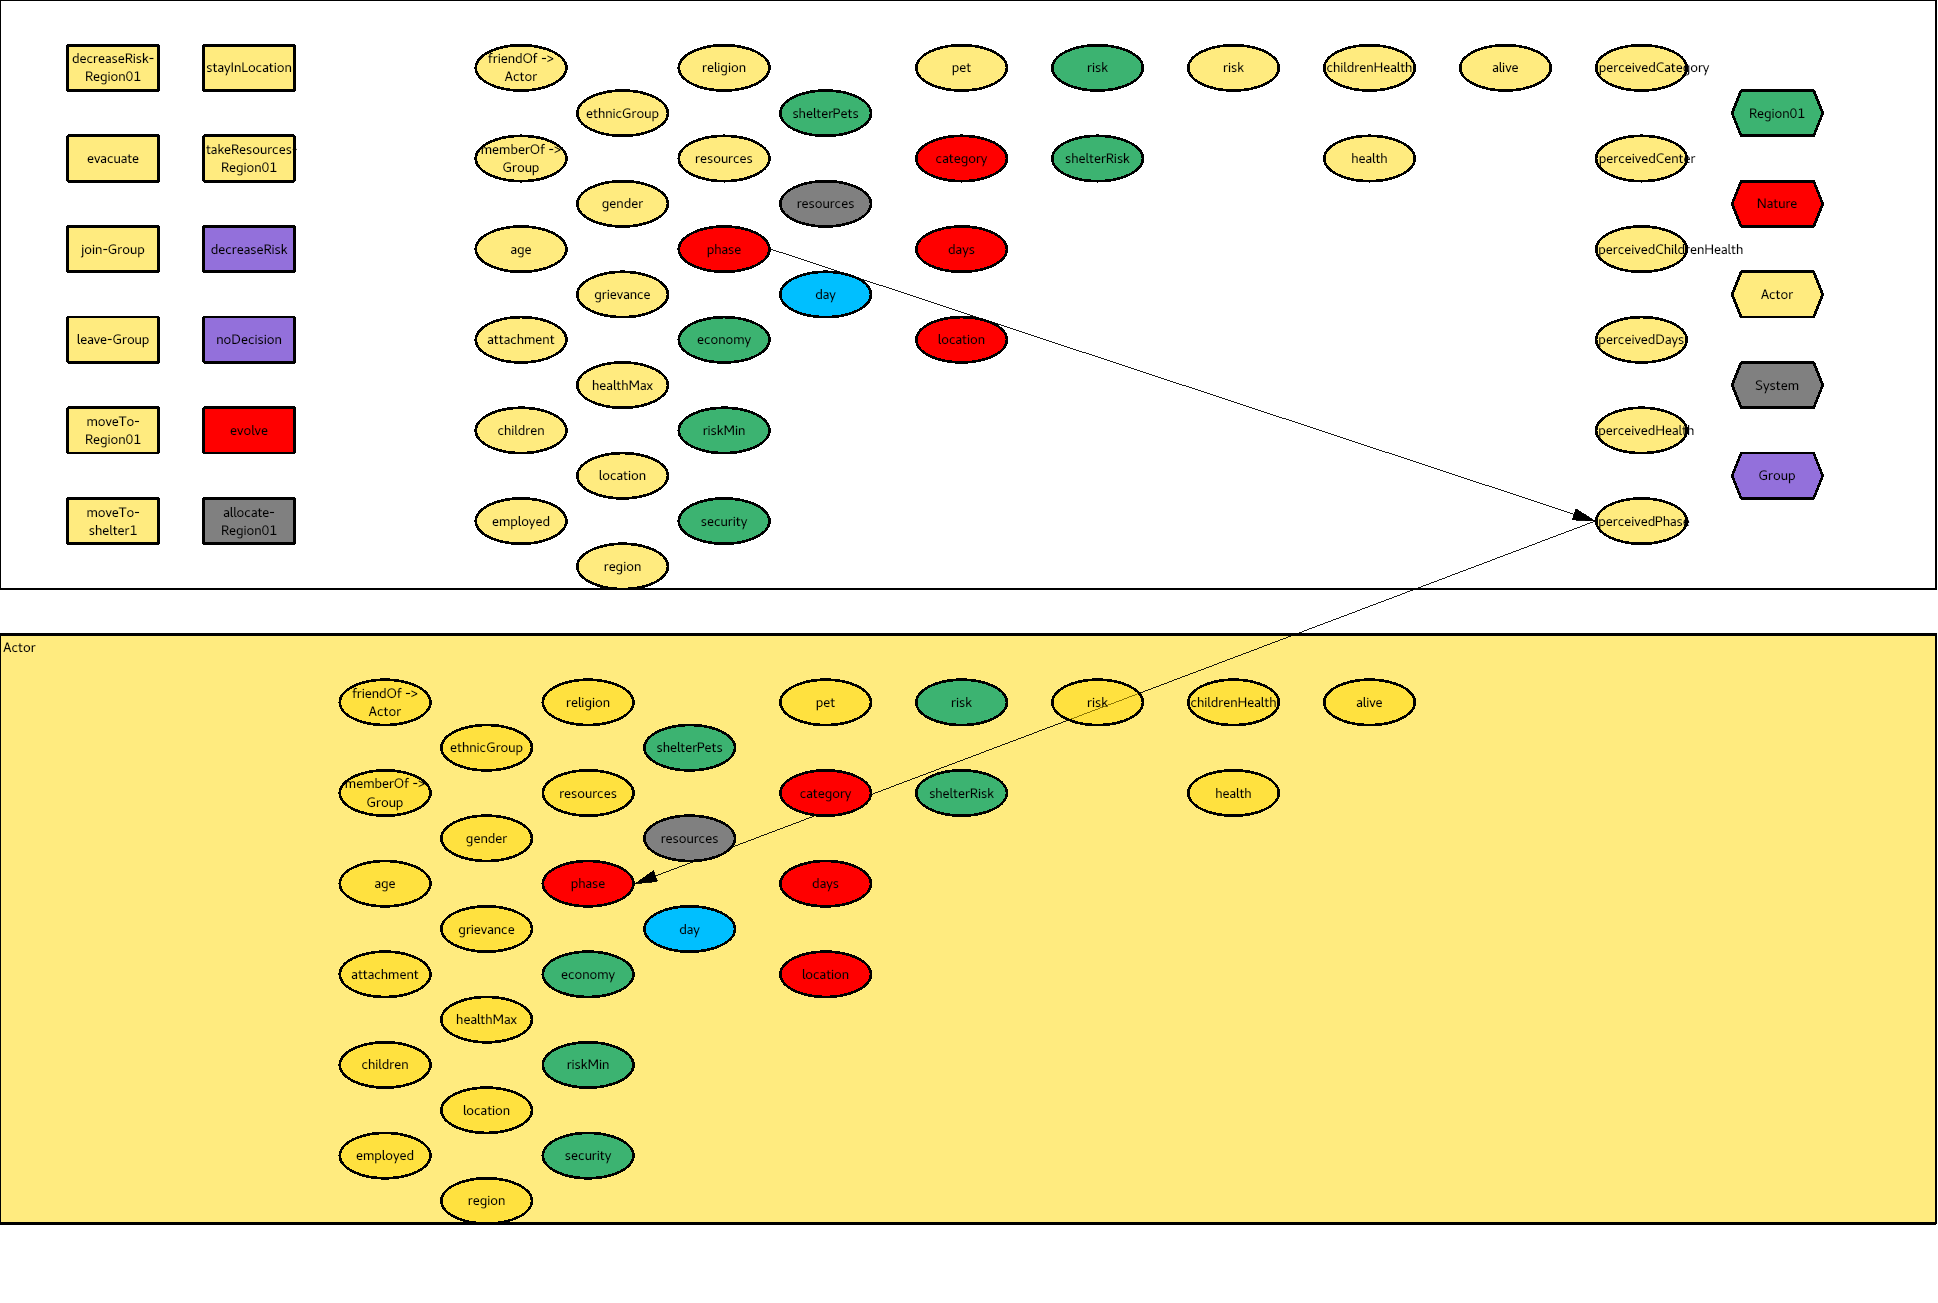
\includegraphics[width=\textwidth]{images/perceivedPhaseOfActor.png}%
\begin{flushleft}%
\verb|psychsim/domains/groundtruth/simulation/actor.py:668|%
\end{flushleft}%
\subsubsection{Default observation of Actor's perceivedPhase}%
\label{ssubsec:Default observation of Actor's perceivedPhase}%
\begin{flushleft}%
$\mbox{\textbf{Actor's perceivedPhase}} '$%
$\leftarrow$%
\textbf{Nature's phase}%
\end{flushleft}

%
\subsection{Actor's pet}%
\label{subsec:Actor's pet}%
Owns a pet%
\begin{description}%
\item[Type:]%
Boolean%
\end{description}%
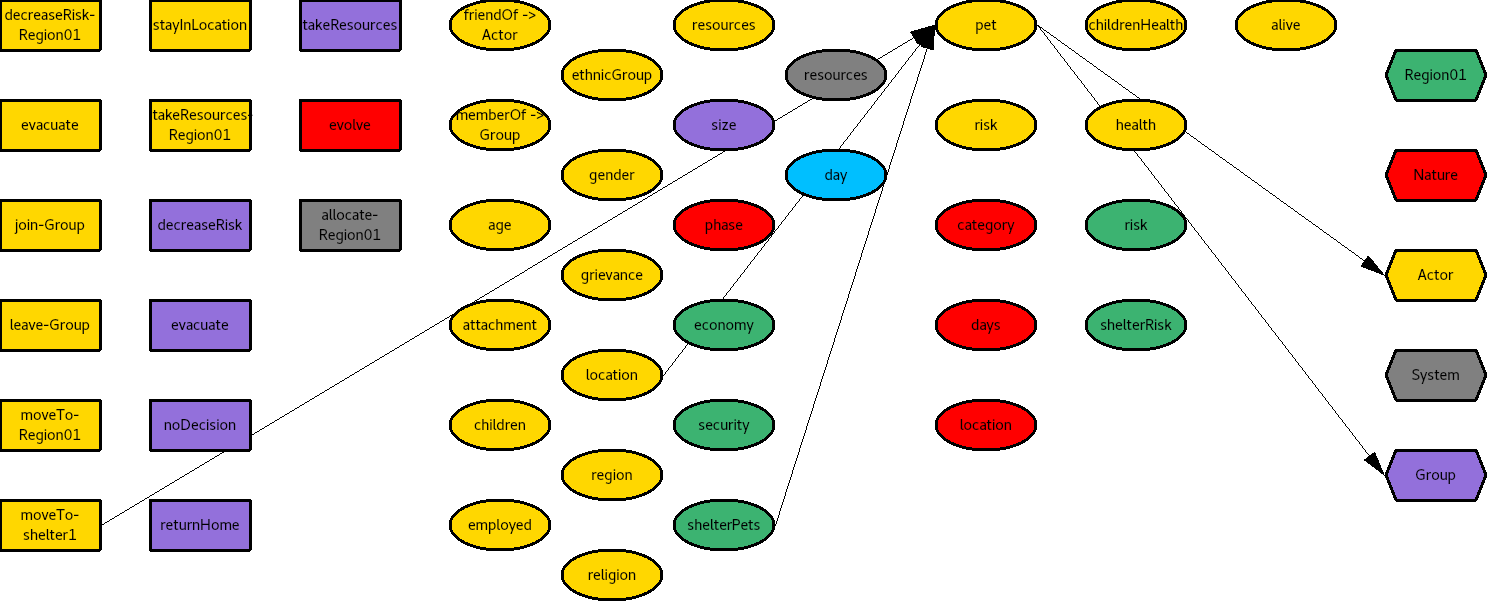
\includegraphics[width=\textwidth]{images/petOfActor.png}%
\begin{flushleft}%
\verb|psychsim/domains/groundtruth/simulation/actor.py:102|%
\end{flushleft}%
\subsubsection{Effect of Actor{-}moveTo{-}shelter1 on Actor's pet}%
\label{ssubsec:Effect of Actor{-}moveTo{-}shelter1 on Actor's pet}%
\begin{flushleft}%
\verb|psychsim/domains/groundtruth/simulation/actor.py:610|%
\linebreak%
IF %
$\mbox{\textbf{Actor's location}} '$%
$=$%
\textbf{shelter1}%
\linebreak%
\hspace*{2em}%
THEN %
: %
IF %
\textbf{Region01's shelterPets}%
\linebreak%
\hspace*{4em}%
THEN %
: %
$\mbox{\textbf{Actor's pet}} '$%
$\leftarrow$%
\textbf{Actor's pet}%
\linebreak%
\hspace*{4em}%
ELSE %
: %
$\mbox{\textbf{Actor's pet}} '$%
$\leftarrow$%
\textbf{false}%
\linebreak%
\hspace*{2em}%
ELSE %
: %
$\mbox{\textbf{Actor's pet}} '$%
$\leftarrow$%
\textbf{Actor's pet}%
\end{flushleft}

%
\subsection{Actor's region}%
\label{subsec:Actor's region}%
Region of residence%
\begin{description}%
\item[Type:]%
String%
\item[Values:]%
\textbf{Region01}%
\end{description}%
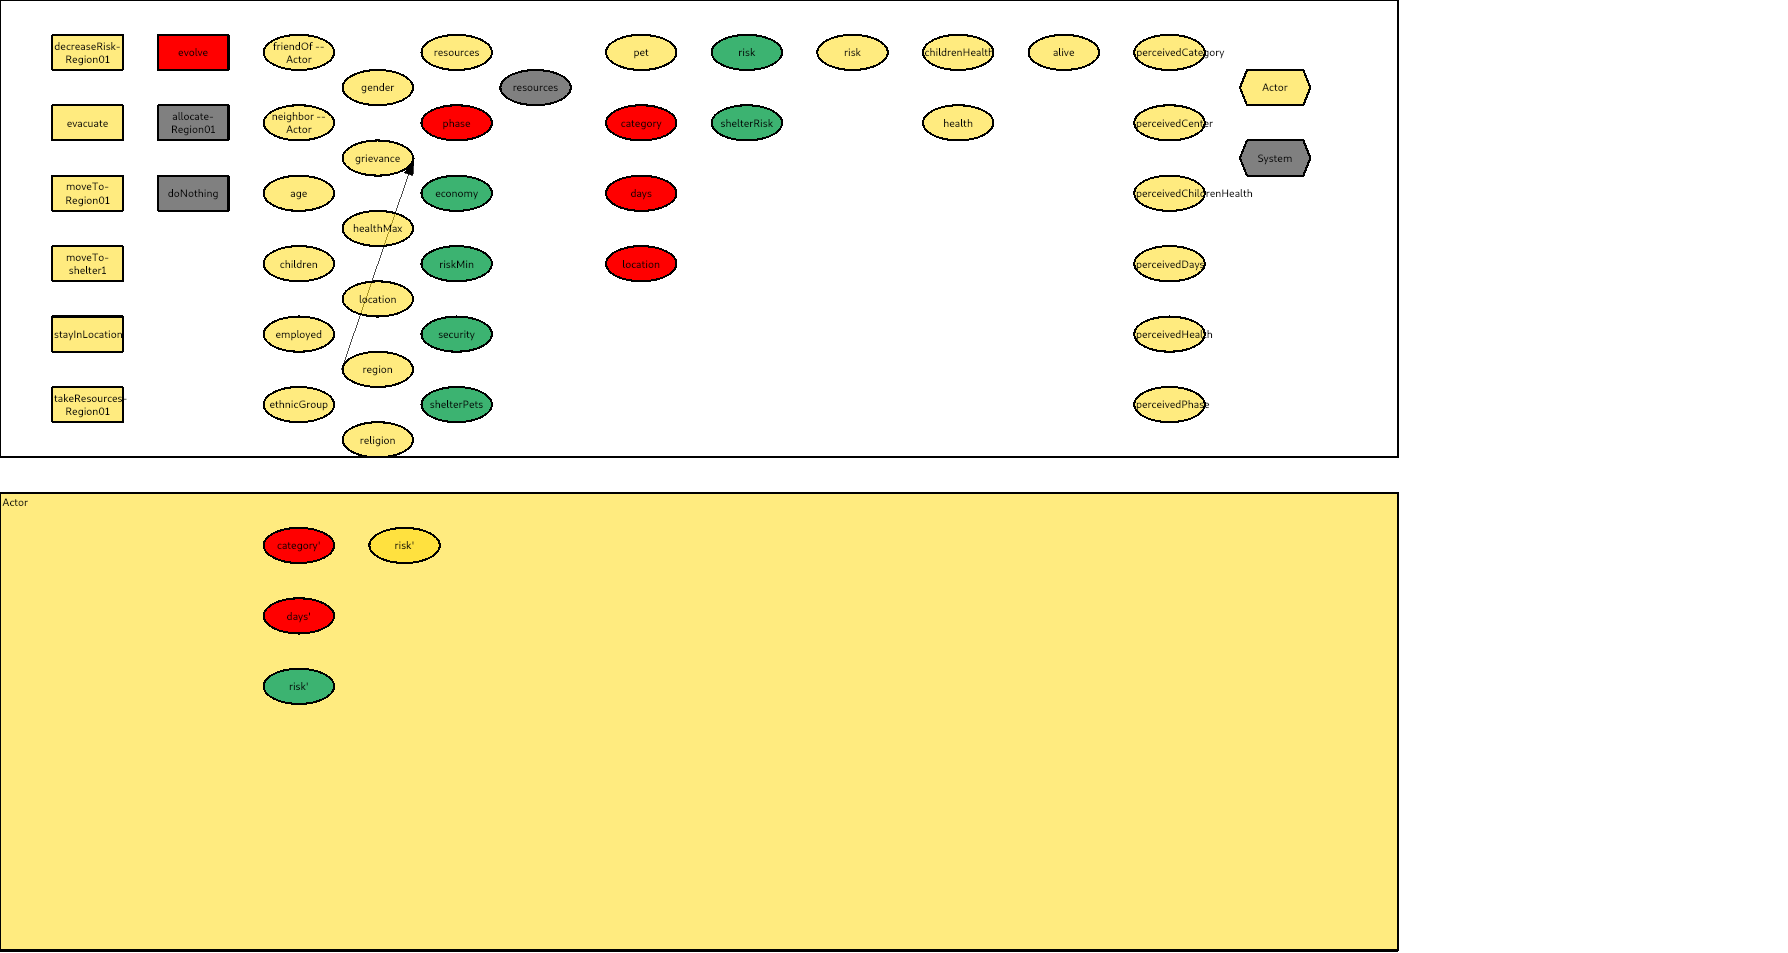
\includegraphics[width=\textwidth]{images/regionOfActor.png}%
\begin{flushleft}%
\verb|psychsim/domains/groundtruth/simulation/actor.py:164|%
\end{flushleft}

%
\subsection{Actor's religion}%
\label{subsec:Actor's religion}%
Religious affiliation of actor%
\begin{description}%
\item[Type:]%
String%
\item[Values:]%
\textbf{majority}%
, %
\textbf{minority}%
, %
\textbf{none}%
\end{description}%
\begin{flushleft}%
\verb|psychsim/domains/groundtruth/simulation/actor.py:61|%
\end{flushleft}

%
\subsection{Actor's resources}%
\label{subsec:Actor's resources}%
Material resources (wealth) currently owned%
\begin{description}%
\item[Type:]%
Real%
\end{description}%
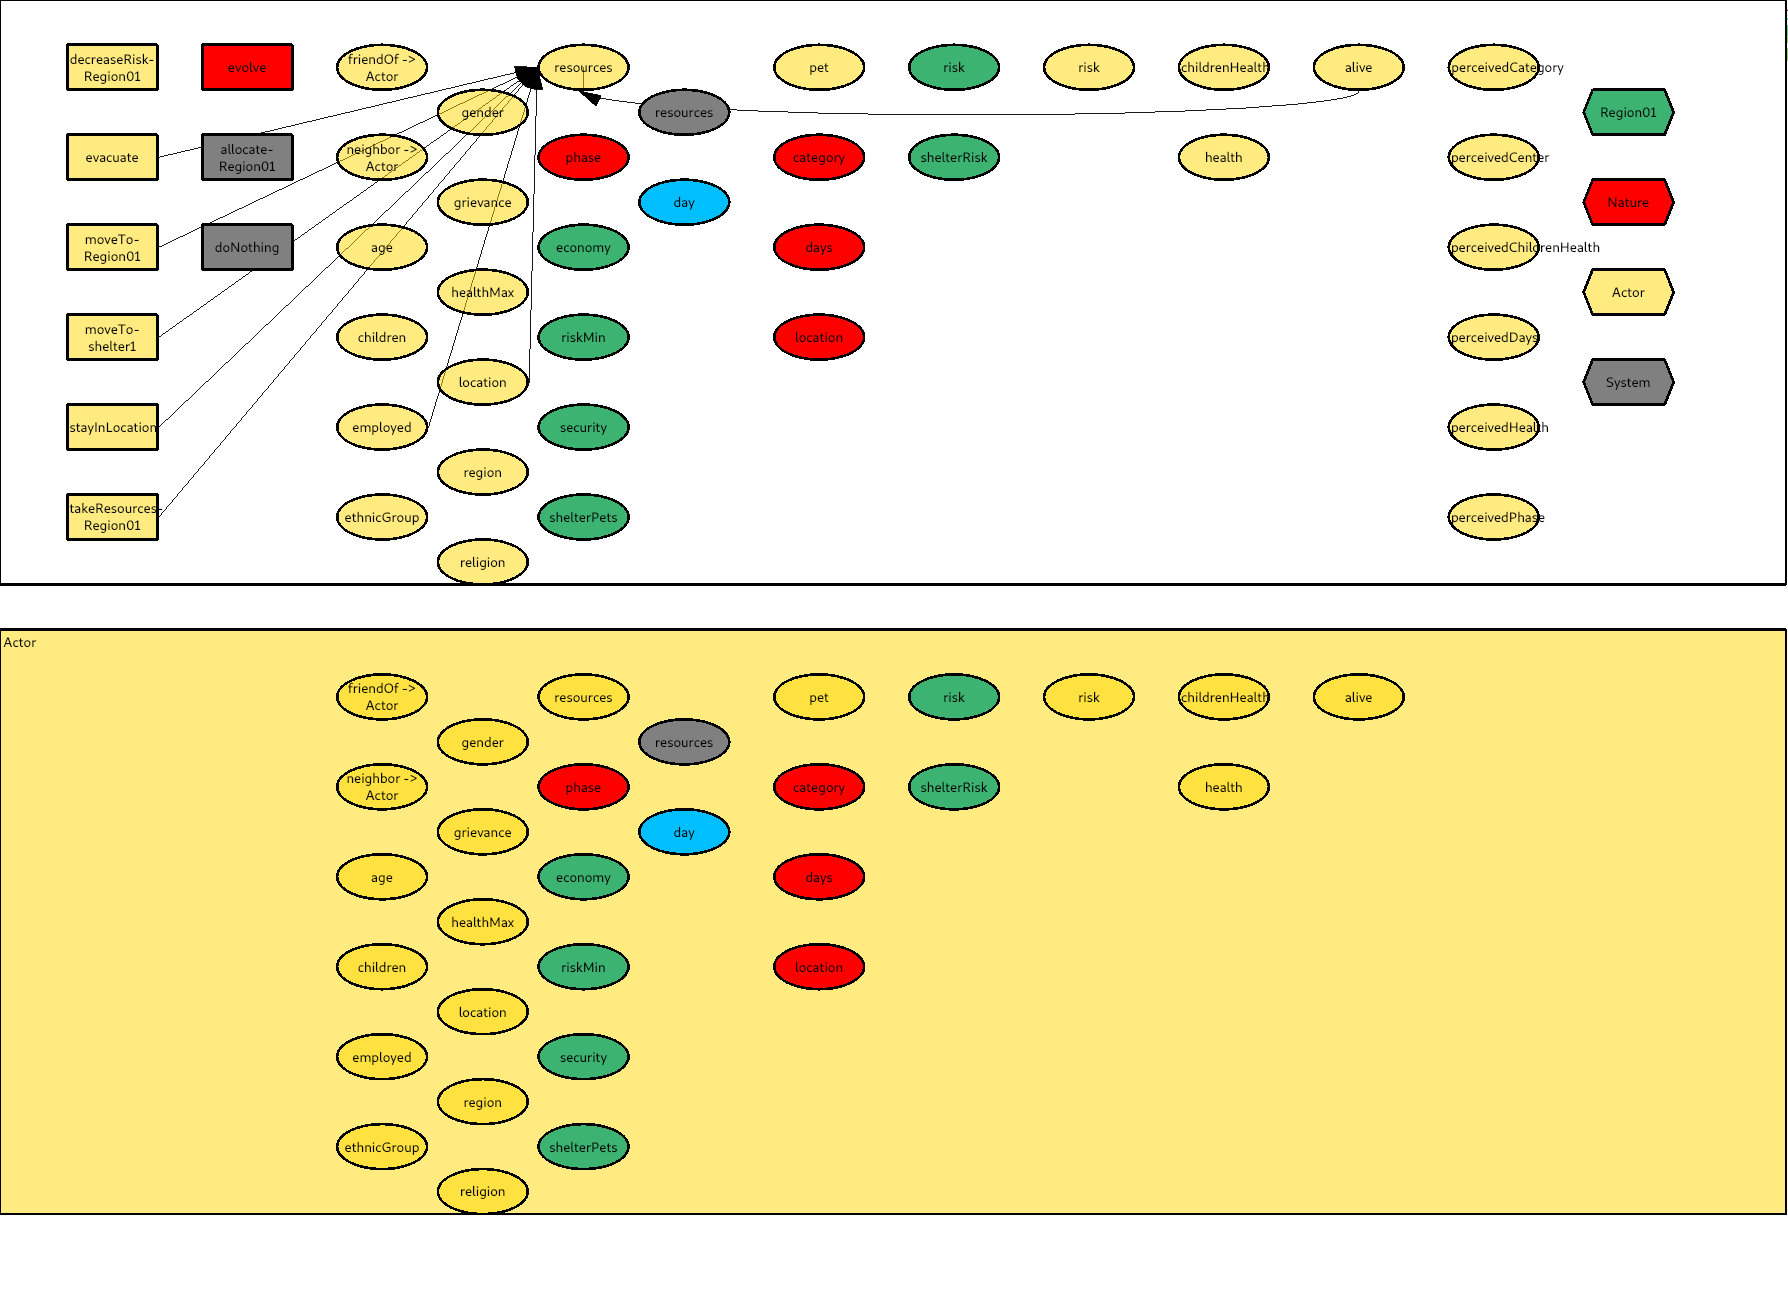
\includegraphics[width=\textwidth]{images/resourcesOfActor.png}%
\begin{flushleft}%
\verb|psychsim/domains/groundtruth/simulation/actor.py:234|%
\end{flushleft}%
\subsubsection{Effect of Actor{-}evacuate on Actor's resources}%
\label{ssubsec:Effect of Actor{-}evacuate on Actor's resources}%
\begin{flushleft}%
\verb|psychsim/domains/groundtruth/simulation/actor.py:534|%
\linebreak%
IF %
\textbf{Actor's resources}%
$>$%
0.40%
\linebreak%
\hspace*{2em}%
THEN %
: %
$\mbox{\textbf{Actor's resources}} '$%
$\leftarrow$%
\textbf{Actor's resources}%
${-}0.40$%
\linebreak%
\hspace*{2em}%
ELSE %
: %
$\mbox{\textbf{Actor's resources}} '$%
$\leftarrow$%
0.00%
\end{flushleft}

%
\subsubsection{Effect of Actor{-}moveTo{-}Region01 on Actor's resources}%
\label{ssubsec:Effect of Actor{-}moveTo{-}Region01 on Actor's resources}%
\begin{flushleft}%
\verb|psychsim/domains/groundtruth/simulation/actor.py:521|%
\linebreak%
IF %
\textbf{Actor's alive}%
\linebreak%
\hspace*{2em}%
THEN %
: %
IF %
\textbf{Actor's employed}%
\linebreak%
\hspace*{4em}%
THEN %
: %
$\mbox{\textbf{Actor's resources}} '$%
$\leftarrow$%
60\%%
$\cdot$%
\textbf{Actor's resources}%
+0.40%
\linebreak%
\hspace*{4em}%
ELSE %
: %
$\mbox{\textbf{Actor's resources}} '$%
$\leftarrow$%
\textbf{Actor's resources}%
\linebreak%
\hspace*{2em}%
ELSE %
: %
$\mbox{\textbf{Actor's resources}} '$%
$\leftarrow$%
\textbf{Actor's resources}%
\end{flushleft}

%
\subsubsection{Effect of Actor{-}moveTo{-}shelter1 on Actor's resources}%
\label{ssubsec:Effect of Actor{-}moveTo{-}shelter1 on Actor's resources}%
\begin{flushleft}%
\verb|psychsim/domains/groundtruth/simulation/actor.py:526|%
\linebreak%
$\mbox{\textbf{Actor's resources}} '$%
$\leftarrow$%
0\%%
$\cdot$%
\textbf{Actor's resources}%
\end{flushleft}

%
\subsubsection{Effect of Actor{-}stayInLocation on Actor's resources}%
\label{ssubsec:Effect of Actor{-}stayInLocation on Actor's resources}%
\begin{flushleft}%
\verb|psychsim/domains/groundtruth/simulation/actor.py:510|%
\linebreak%
IF %
\textbf{Actor's alive}%
\linebreak%
\hspace*{2em}%
THEN %
: %
IF %
\textbf{Actor's employed}%
\linebreak%
\hspace*{4em}%
THEN %
: %
IF %
\textbf{Actor's location}%
$=$%
\textbf{\{'Region01', 'evacuated'\}}%
\linebreak%
\hspace*{6em}%
THEN %
: %
$\mbox{\textbf{Actor's resources}} '$%
$\leftarrow$%
60\%%
$\cdot$%
\textbf{Actor's resources}%
+0.40%
\linebreak%
\hspace*{6em}%
ELSE %
: %
$\mbox{\textbf{Actor's resources}} '$%
$\leftarrow$%
\textbf{Actor's resources}%
\linebreak%
\hspace*{4em}%
ELSE %
: %
$\mbox{\textbf{Actor's resources}} '$%
$\leftarrow$%
\textbf{Actor's resources}%
\linebreak%
\hspace*{2em}%
ELSE %
: %
$\mbox{\textbf{Actor's resources}} '$%
$\leftarrow$%
\textbf{Actor's resources}%
\end{flushleft}

%
\subsubsection{Effect of Actor{-}takeResources{-}Region01 on Actor's resources}%
\label{ssubsec:Effect of Actor{-}takeResources{-}Region01 on Actor's resources}%
\begin{flushleft}%
\verb|psychsim/domains/groundtruth/simulation/actor.py:577|%
\linebreak%
$\mbox{\textbf{Actor's resources}} '$%
$\leftarrow$%
80\%%
$\cdot$%
\textbf{Actor's resources}%
+0.20%
\end{flushleft}

%
\subsection{Actor's risk}%
\label{subsec:Actor's risk}%
Current level of risk from hurricane%
\begin{description}%
\item[Type:]%
Real%
\end{description}%
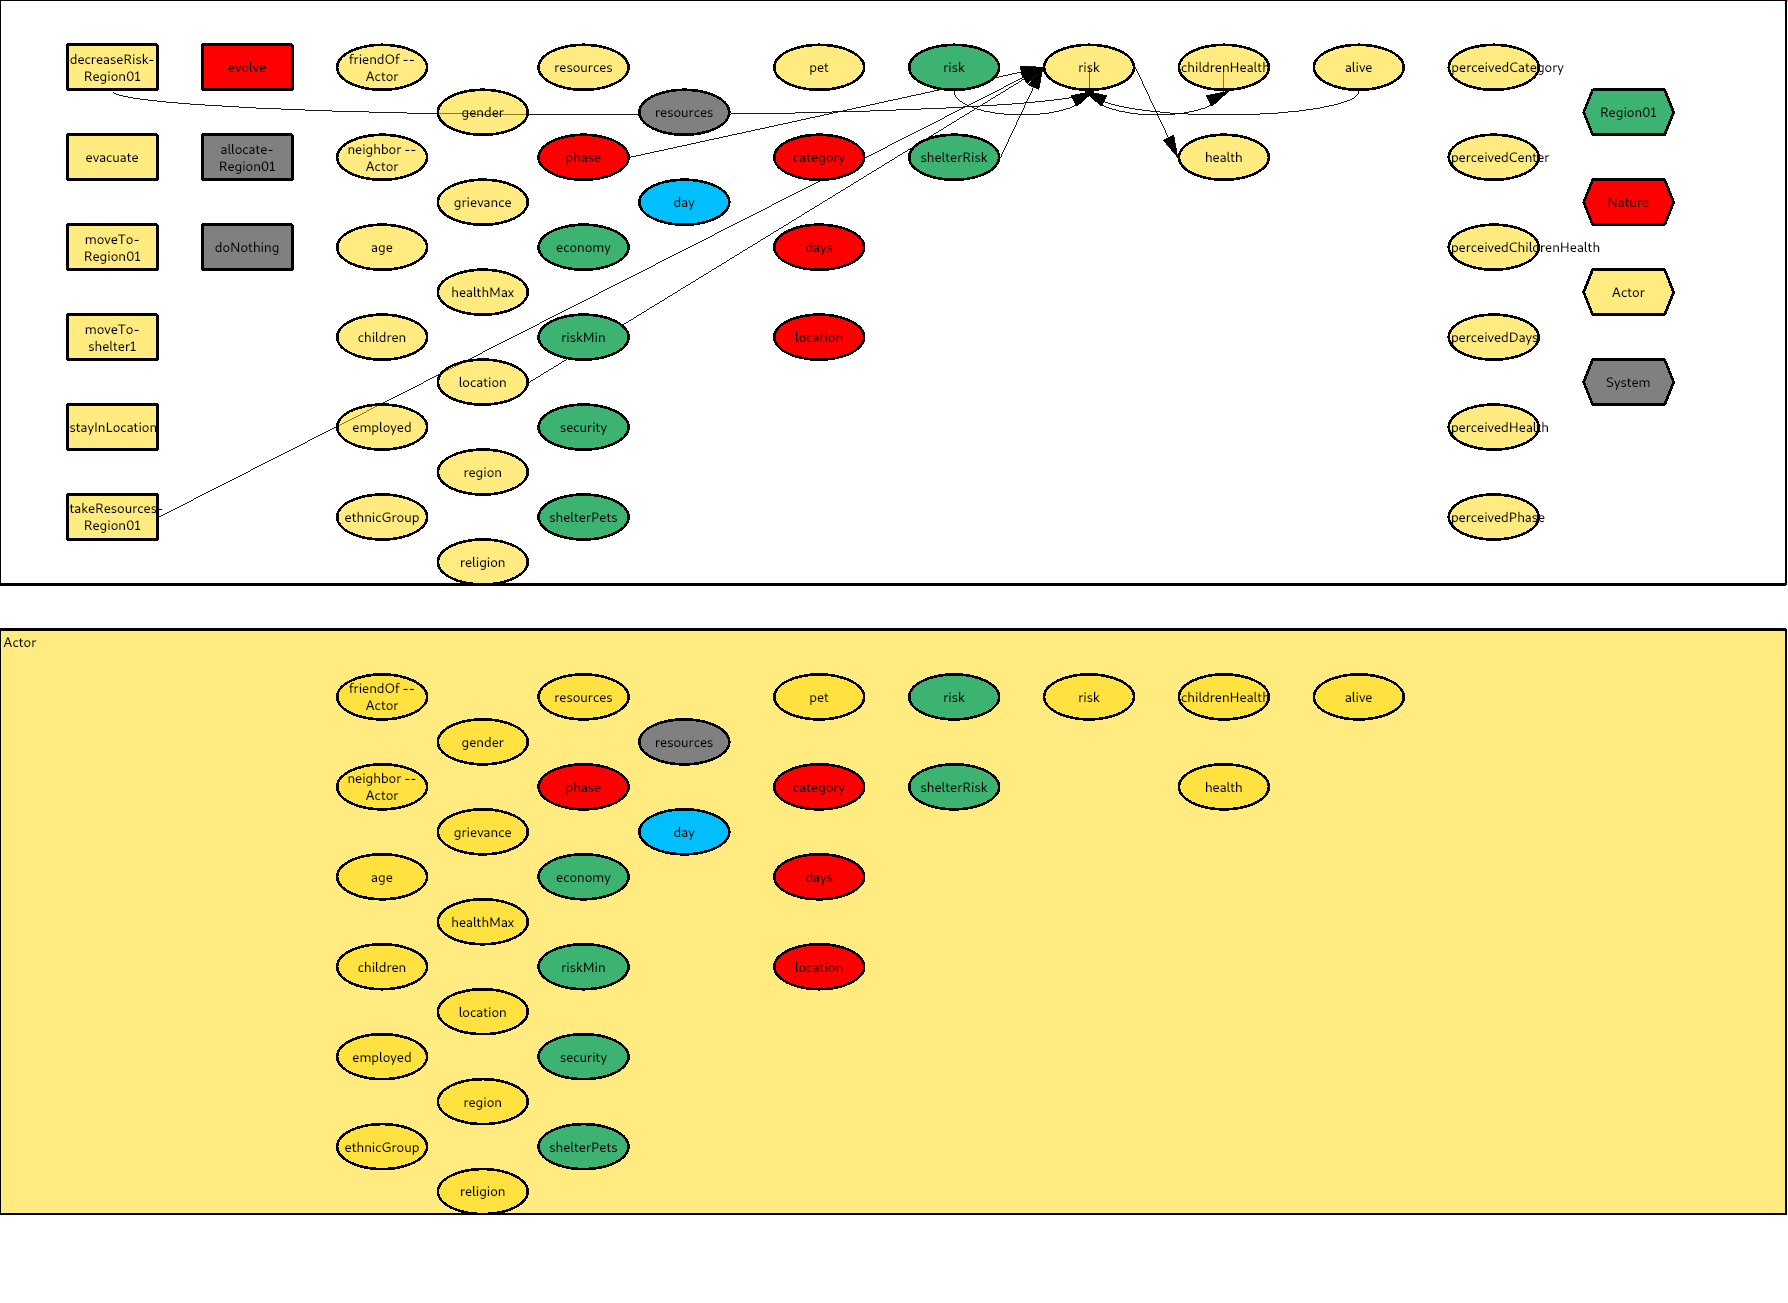
\includegraphics[width=\textwidth]{images/riskOfActor.png}%
\begin{flushleft}%
\verb|psychsim/domains/groundtruth/simulation/actor.py:254|%
\end{flushleft}%
\subsubsection{Effect of Actor{-}decreaseRisk{-}Region01 on Actor's risk}%
\label{ssubsec:Effect of Actor{-}decreaseRisk{-}Region01 on Actor's risk}%
\begin{flushleft}%
\verb|psychsim/domains/groundtruth/simulation/actor.py:559|%
\linebreak%
$\mbox{\textbf{Actor's risk}} '$%
$\leftarrow$%
80\%%
$\cdot$%
\textbf{Actor's risk}%
+0.20%
\end{flushleft}

%
\subsubsection{Effect of Actor{-}takeResources{-}Region01 on Actor's risk}%
\label{ssubsec:Effect of Actor{-}takeResources{-}Region01 on Actor's risk}%
\begin{flushleft}%
\verb|psychsim/domains/groundtruth/simulation/actor.py:584|%
\linebreak%
IF %
\textbf{Nature's phase}%
$=$%
\textbf{none}%
\linebreak%
\hspace*{2em}%
THEN %
: %
$\mbox{\textbf{Actor's risk}} '$%
$\leftarrow$%
19\%%
$\cdot$%
\textbf{Actor's risk}%
+0.80%
\linebreak%
\hspace*{2em}%
ELSE %
: %
$\mbox{\textbf{Actor's risk}} '$%
$\leftarrow$%
40\%%
$\cdot$%
\textbf{Actor's risk}%
+0.60%
\end{flushleft}

%
\subsubsection{Default change in Actor's risk}%
\label{ssubsec:Default change in Actor's risk}%
\begin{flushleft}%
\verb|psychsim/domains/groundtruth/simulation/actor.py:450|%
\linebreak%
IF %
\textbf{Actor's alive}%
\linebreak%
\hspace*{2em}%
THEN %
: %
IF %
$\mbox{\textbf{Actor's location}} '$%
$=$%
\textbf{shelter1}%
\linebreak%
\hspace*{4em}%
THEN %
: %
$\mbox{\textbf{Actor's risk}} '$%
$\leftarrow$%
\textbf{Region01's shelterRisk}%
\linebreak%
\hspace*{4em}%
ELSE %
: %
IF %
$\mbox{\textbf{Actor's location}} '$%
$=$%
\textbf{evacuated}%
\linebreak%
\hspace*{6em}%
THEN %
: %
$\mbox{\textbf{Actor's risk}} '$%
$\leftarrow$%
9\%%
$\cdot$%
\textbf{Actor's risk}%
\linebreak%
\hspace*{6em}%
ELSE %
: %
$\mbox{\textbf{Actor's risk}} '$%
$\leftarrow$%
$\mbox{\textbf{Region01's risk}} '$%
\linebreak%
\hspace*{2em}%
ELSE %
: %
$\mbox{\textbf{Actor's risk}} '$%
$\leftarrow$%
0.00%
\end{flushleft}

%
\subsection{Nature's category}%
\label{subsec:Nature's category}%
\begin{description}%
\item[Type:]%
Integer%
\end{description}%
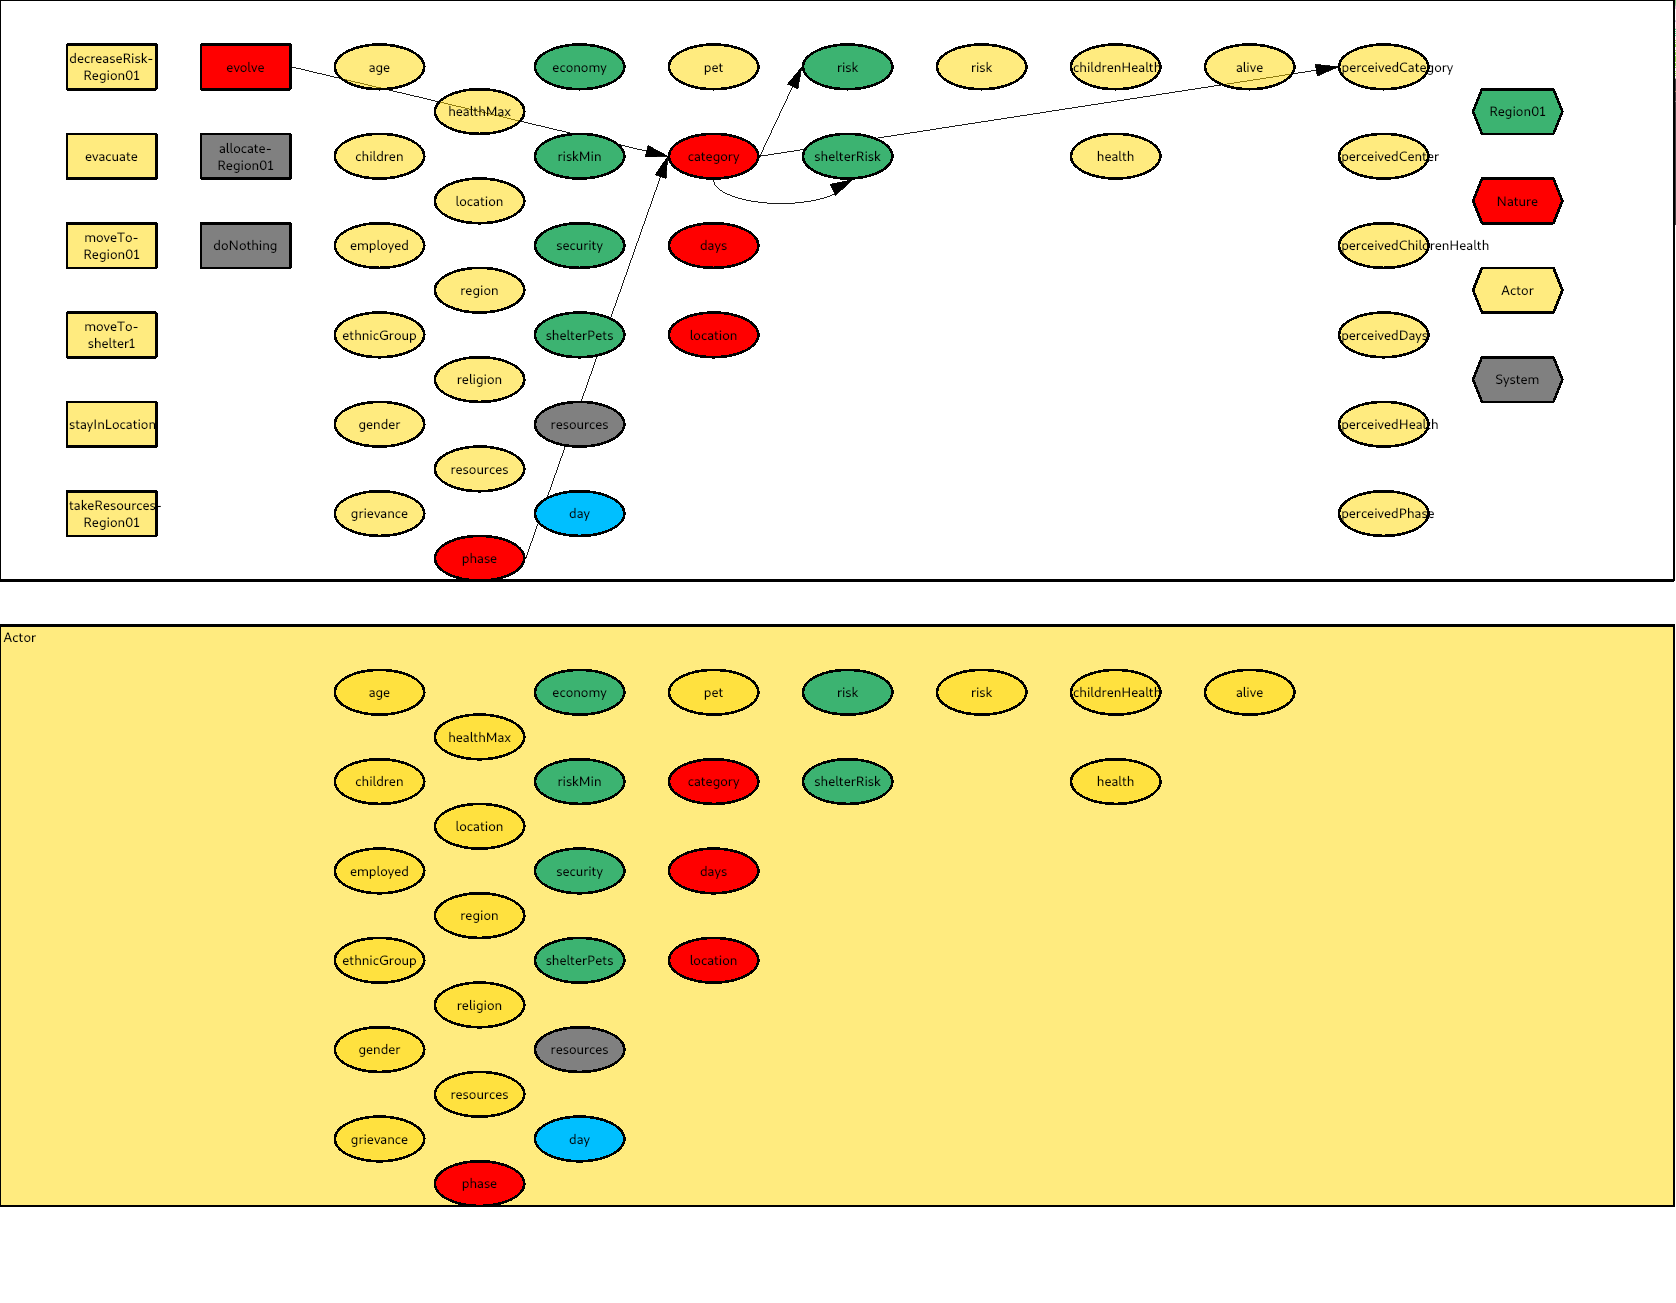
\includegraphics[width=\textwidth]{images/categoryOfNature.png}%
\begin{flushleft}%
\verb|psychsim/domains/groundtruth/simulation/nature.py:26|%
\end{flushleft}%
\subsubsection{Effect of Nature{-}evolve on Nature's category}%
\label{ssubsec:Effect of Nature{-}evolve on Nature's category}%
\begin{flushleft}%
\verb|psychsim/domains/groundtruth/simulation/nature.py:80|%
\linebreak%
IF %
$\mbox{\textbf{Nature's phase}} '$%
\linebreak%
\hspace*{2em}%
$= \mbox{\textbf{approaching}}$%
: %
IF %
\textbf{Nature's category}%
$=$%
0%
\linebreak%
\hspace*{4em}%
THEN %
: %
\linebreak%
\hspace*{6em}%
20\%%
: %
$\mbox{\textbf{Nature's category}} '$%
$\leftarrow$%
1%
\linebreak%
\hspace*{6em}%
20\%%
: %
$\mbox{\textbf{Nature's category}} '$%
$\leftarrow$%
2%
\linebreak%
\hspace*{6em}%
20\%%
: %
$\mbox{\textbf{Nature's category}} '$%
$\leftarrow$%
3%
\linebreak%
\hspace*{6em}%
20\%%
: %
$\mbox{\textbf{Nature's category}} '$%
$\leftarrow$%
4%
\linebreak%
\hspace*{6em}%
20\%%
: %
$\mbox{\textbf{Nature's category}} '$%
$\leftarrow$%
5%
\linebreak%
\hspace*{4em}%
ELSE %
: %
IF %
\textbf{Nature's category}%
$=$%
1%
\linebreak%
\hspace*{6em}%
THEN %
: %
\linebreak%
\hspace*{8em}%
60\%%
: %
$\mbox{\textbf{Nature's category}} '$%
$\leftarrow$%
\textbf{Nature's category}%
\linebreak%
\hspace*{8em}%
40\%%
: %
$\mbox{\textbf{Nature's category}} '$%
$\leftarrow$%
2%
\linebreak%
\hspace*{6em}%
ELSE %
: %
IF %
\textbf{Nature's category}%
$=$%
5%
\linebreak%
\hspace*{8em}%
THEN %
: %
\linebreak%
\hspace*{10em}%
40\%%
: %
$\mbox{\textbf{Nature's category}} '$%
$\leftarrow$%
4%
\linebreak%
\hspace*{10em}%
60\%%
: %
$\mbox{\textbf{Nature's category}} '$%
$\leftarrow$%
\textbf{Nature's category}%
\linebreak%
\hspace*{8em}%
ELSE %
: %
\linebreak%
\hspace*{10em}%
20\%%
: %
$\mbox{\textbf{Nature's category}} '$%
$\leftarrow$%
\textbf{Nature's category}%
${-}1$%
\linebreak%
\hspace*{10em}%
60\%%
: %
$\mbox{\textbf{Nature's category}} '$%
$\leftarrow$%
\textbf{Nature's category}%
\linebreak%
\hspace*{10em}%
20\%%
: %
$\mbox{\textbf{Nature's category}} '$%
$\leftarrow$%
\textbf{Nature's category}%
+1%
\linebreak%
\hspace*{2em}%
$= \mbox{\textbf{active}}$%
: %
$\mbox{\textbf{Nature's category}} '$%
$\leftarrow$%
\textbf{Nature's category}%
\linebreak%
\hspace*{2em}%
$= \mbox{\textbf{none}}$%
: %
$\mbox{\textbf{Nature's category}} '$%
$\leftarrow$%
0%
\end{flushleft}

%
\subsection{Nature's days}%
\label{subsec:Nature's days}%
\begin{description}%
\item[Type:]%
Integer%
\end{description}%
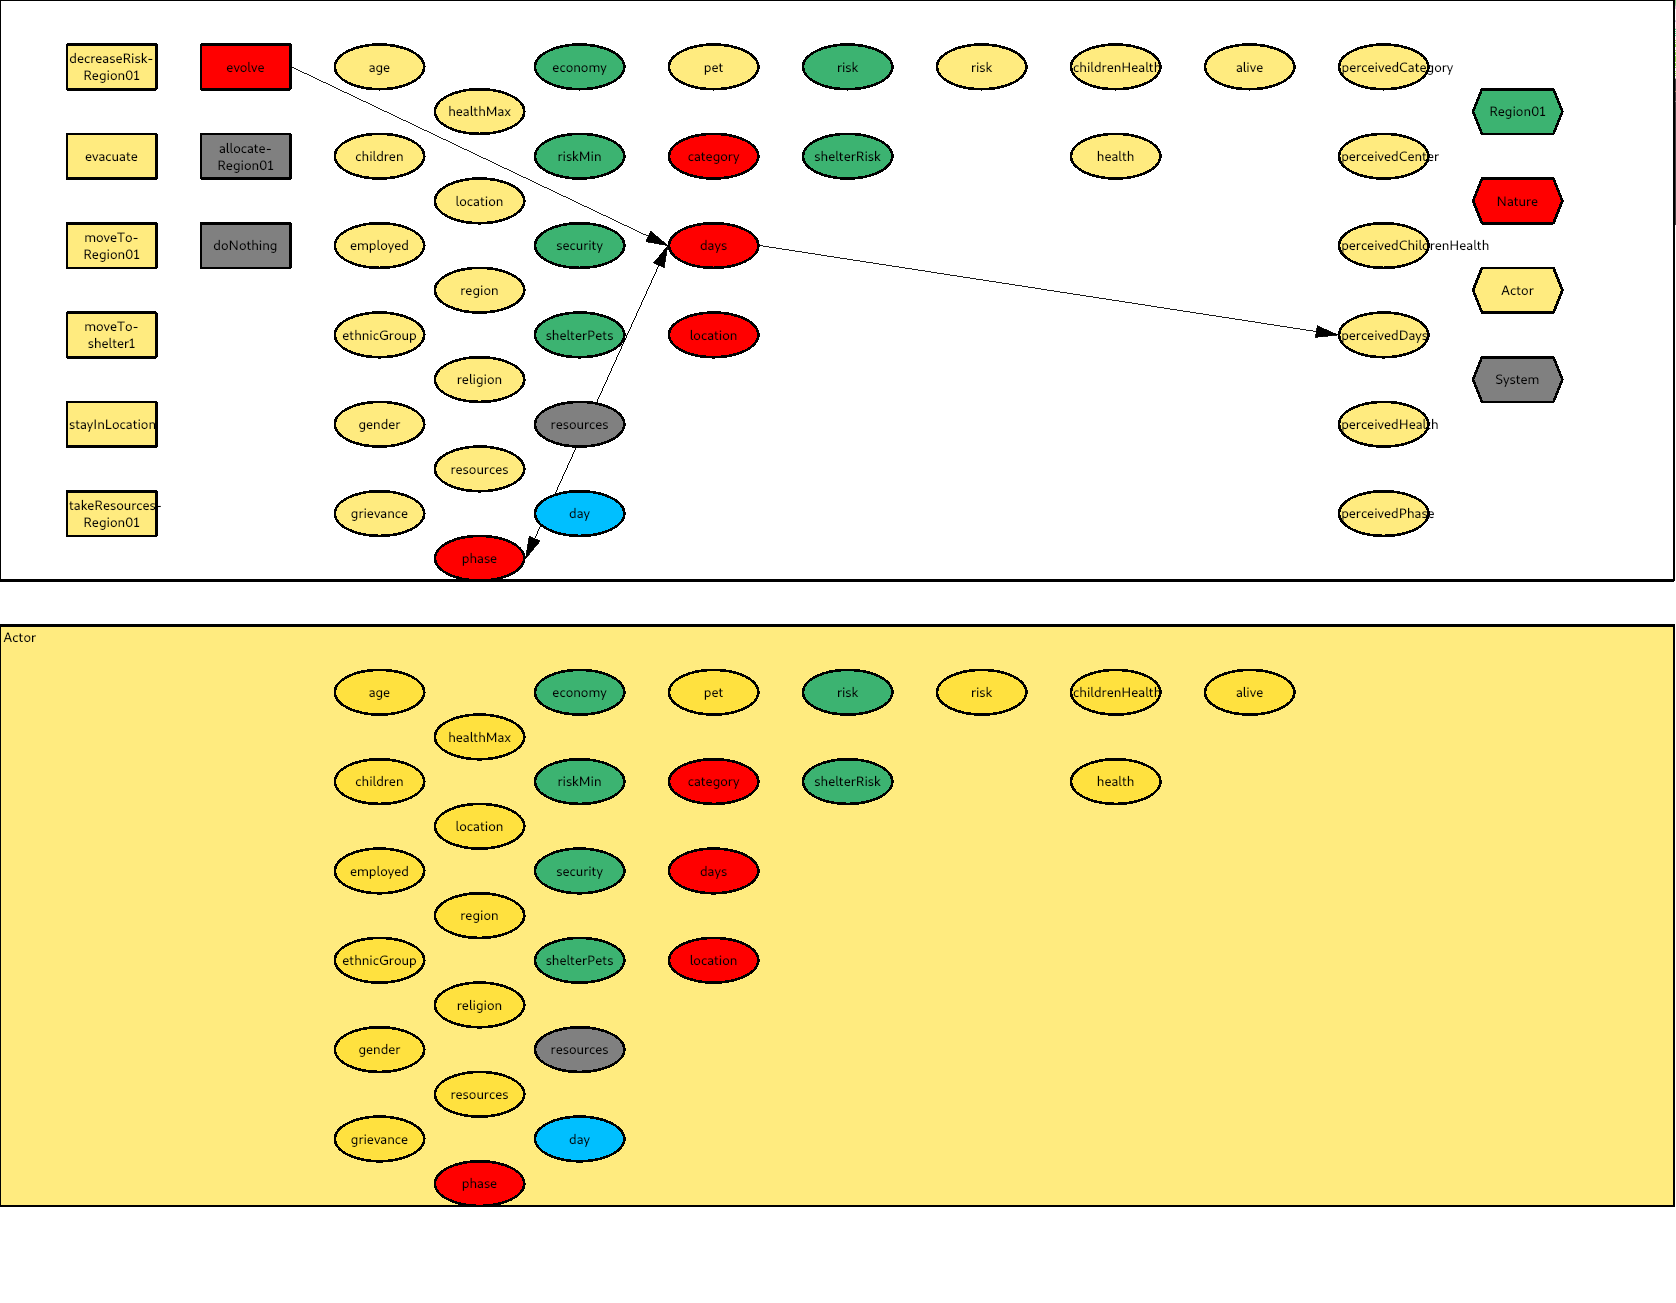
\includegraphics[width=\textwidth]{images/daysOfNature.png}%
\begin{flushleft}%
\verb|psychsim/domains/groundtruth/simulation/nature.py:18|%
\end{flushleft}%
\subsubsection{Effect of Nature{-}evolve on Nature's days}%
\label{ssubsec:Effect of Nature{-}evolve on Nature's days}%
\begin{flushleft}%
\verb|psychsim/domains/groundtruth/simulation/nature.py:54|%
\linebreak%
IF %
\textbf{Nature's phase}%
$=$%
$\mbox{\textbf{Nature's phase}} '$%
\linebreak%
\hspace*{2em}%
THEN %
: %
$\mbox{\textbf{Nature's days}} '$%
$\leftarrow$%
\textbf{Nature's days}%
+1%
\linebreak%
\hspace*{2em}%
ELSE %
: %
$\mbox{\textbf{Nature's days}} '$%
$\leftarrow$%
0%
\end{flushleft}

%
\subsection{Nature's location}%
\label{subsec:Nature's location}%
\begin{description}%
\item[Type:]%
String%
\item[Values:]%
\textbf{Region01}%
, %
\textbf{none}%
\end{description}%
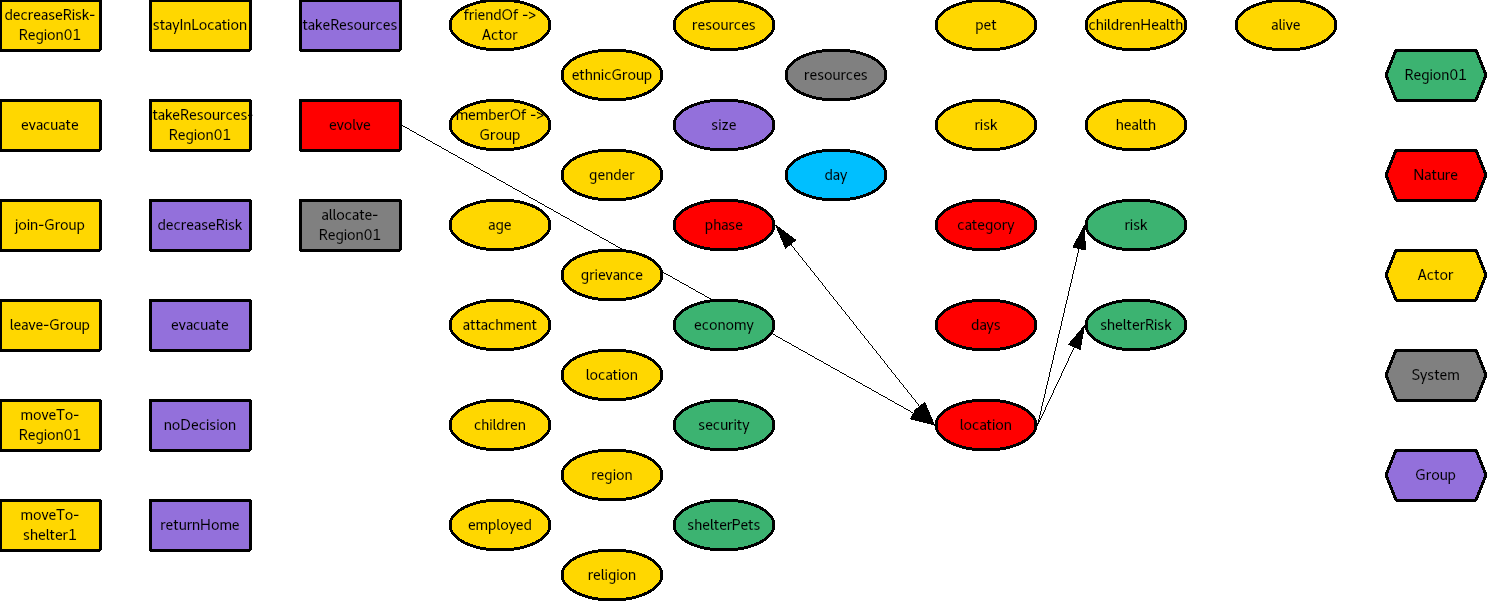
\includegraphics[width=\textwidth]{images/locationOfNature.png}%
\begin{flushleft}%
\verb|psychsim/domains/groundtruth/simulation/nature.py:23|%
\end{flushleft}%
\subsubsection{Effect of Nature{-}evolve on Nature's location}%
\label{ssubsec:Effect of Nature{-}evolve on Nature's location}%
\begin{flushleft}%
\verb|psychsim/domains/groundtruth/simulation/nature.py:113|%
\linebreak%
IF %
$\mbox{\textbf{Nature's phase}} '$%
\linebreak%
\hspace*{2em}%
$= \mbox{\textbf{approaching}}$%
: %
IF %
\textbf{Nature's location}%
$=$%
\textbf{none}%
\linebreak%
\hspace*{4em}%
THEN %
: %
$\mbox{\textbf{Nature's location}} '$%
$\leftarrow$%
\textbf{Region01}%
\linebreak%
\hspace*{4em}%
ELSE %
: %
$\mbox{\textbf{Nature's location}} '$%
$\leftarrow$%
\textbf{Nature's location}%
\linebreak%
\hspace*{2em}%
$= \mbox{\textbf{active}}$%
: %
IF %
\textbf{Nature's phase}%
$=$%
\textbf{approaching}%
\linebreak%
\hspace*{4em}%
THEN %
: %
$\mbox{\textbf{Nature's location}} '$%
$\leftarrow$%
\textbf{Nature's location}%
\linebreak%
\hspace*{4em}%
ELSE %
: %
IF %
\textbf{Nature's location}%
\linebreak%
\hspace*{6em}%
OTHERWISE %
: %
$\mbox{\textbf{Nature's location}} '$%
$\leftarrow$%
\textbf{Nature's location}%
\linebreak%
\hspace*{6em}%
$= \mbox{\textbf{Region01}}$%
: %
\linebreak%
\hspace*{8em}%
20\%%
: %
$\mbox{\textbf{Nature's location}} '$%
$\leftarrow$%
\textbf{Region01}%
\linebreak%
\hspace*{8em}%
48\%%
: %
$\mbox{\textbf{Nature's location}} '$%
$\leftarrow$%
\textbf{none}%
\linebreak%
\hspace*{2em}%
$= \mbox{\textbf{none}}$%
: %
$\mbox{\textbf{Nature's location}} '$%
$\leftarrow$%
\textbf{none}%
\end{flushleft}

%
\subsection{Nature's phase}%
\label{subsec:Nature's phase}%
\begin{description}%
\item[Type:]%
String%
\item[Values:]%
\textbf{active}%
, %
\textbf{approaching}%
, %
\textbf{none}%
\end{description}%
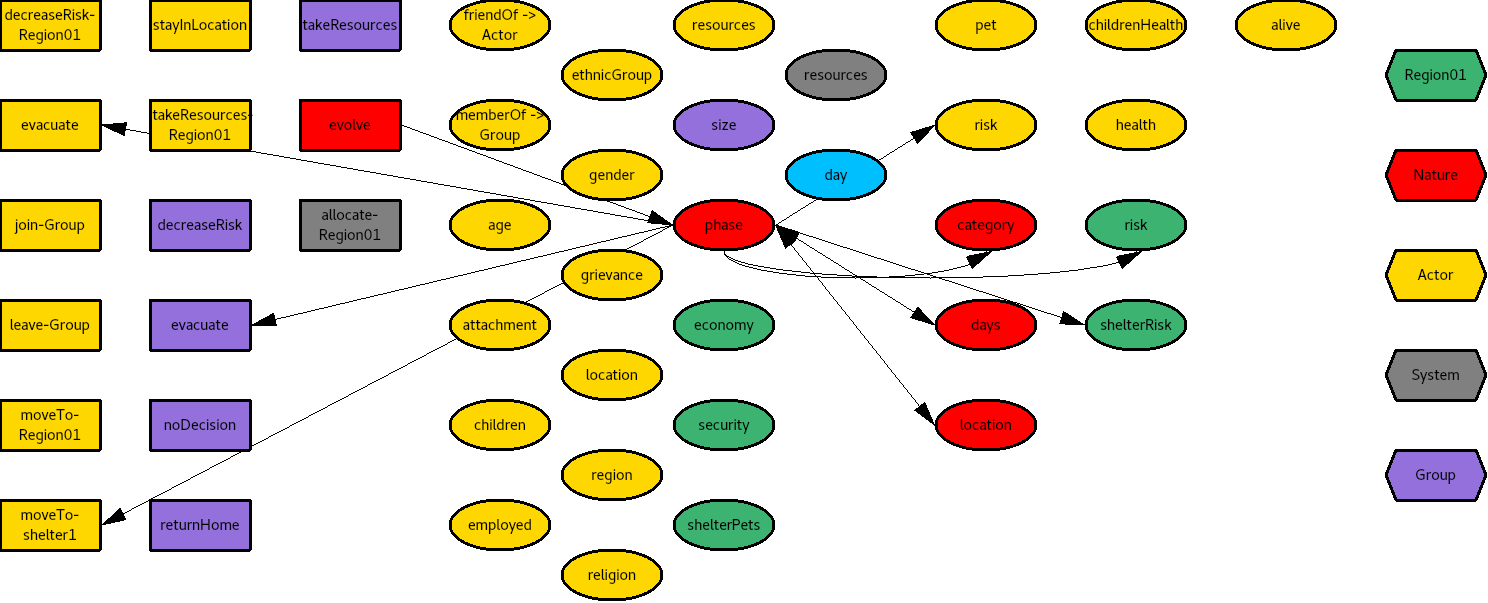
\includegraphics[width=\textwidth]{images/phaseOfNature.png}%
\begin{flushleft}%
\verb|psychsim/domains/groundtruth/simulation/nature.py:16|%
\end{flushleft}%
\subsubsection{Effect of Nature{-}evolve on Nature's phase}%
\label{ssubsec:Effect of Nature{-}evolve on Nature's phase}%
\begin{flushleft}%
\verb|psychsim/domains/groundtruth/simulation/nature.py:49|%
\linebreak%
IF %
\textbf{Nature's phase}%
\linebreak%
\hspace*{2em}%
$= \mbox{\textbf{none}}$%
: %
IF %
\textbf{Nature's days}%
$>$%
2%
\linebreak%
\hspace*{4em}%
THEN %
: %
\linebreak%
\hspace*{6em}%
60\%%
: %
$\mbox{\textbf{Nature's phase}} '$%
$\leftarrow$%
\textbf{approaching}%
\linebreak%
\hspace*{6em}%
40\%%
: %
$\mbox{\textbf{Nature's phase}} '$%
$\leftarrow$%
\textbf{none}%
\linebreak%
\hspace*{4em}%
ELSE %
: %
$\mbox{\textbf{Nature's phase}} '$%
$\leftarrow$%
\textbf{none}%
\linebreak%
\hspace*{2em}%
$= \mbox{\textbf{approaching}}$%
: %
IF %
\textbf{Nature's days}%
$>$%
2%
\linebreak%
\hspace*{4em}%
THEN %
: %
\linebreak%
\hspace*{6em}%
60\%%
: %
$\mbox{\textbf{Nature's phase}} '$%
$\leftarrow$%
\textbf{active}%
\linebreak%
\hspace*{6em}%
40\%%
: %
$\mbox{\textbf{Nature's phase}} '$%
$\leftarrow$%
\textbf{approaching}%
\linebreak%
\hspace*{4em}%
ELSE %
: %
$\mbox{\textbf{Nature's phase}} '$%
$\leftarrow$%
\textbf{approaching}%
\linebreak%
\hspace*{2em}%
OTHERWISE %
: %
IF %
\textbf{Nature's location}%
$=$%
\textbf{none}%
\linebreak%
\hspace*{4em}%
THEN %
: %
$\mbox{\textbf{Nature's phase}} '$%
$\leftarrow$%
\textbf{none}%
\linebreak%
\hspace*{4em}%
ELSE %
: %
$\mbox{\textbf{Nature's phase}} '$%
$\leftarrow$%
\textbf{active}%
\end{flushleft}

%
\subsection{Region01's economy}%
\label{subsec:Region01's economy}%
Current economic level of region%
\begin{description}%
\item[Type:]%
Real%
\end{description}%
\begin{flushleft}%
\verb|psychsim/domains/groundtruth/simulation/region.py:83|%
\end{flushleft}

%
\subsection{Region01's risk}%
\label{subsec:Region01's risk}%
Level of risk from hurricane%
\begin{description}%
\item[Type:]%
Real%
\end{description}%
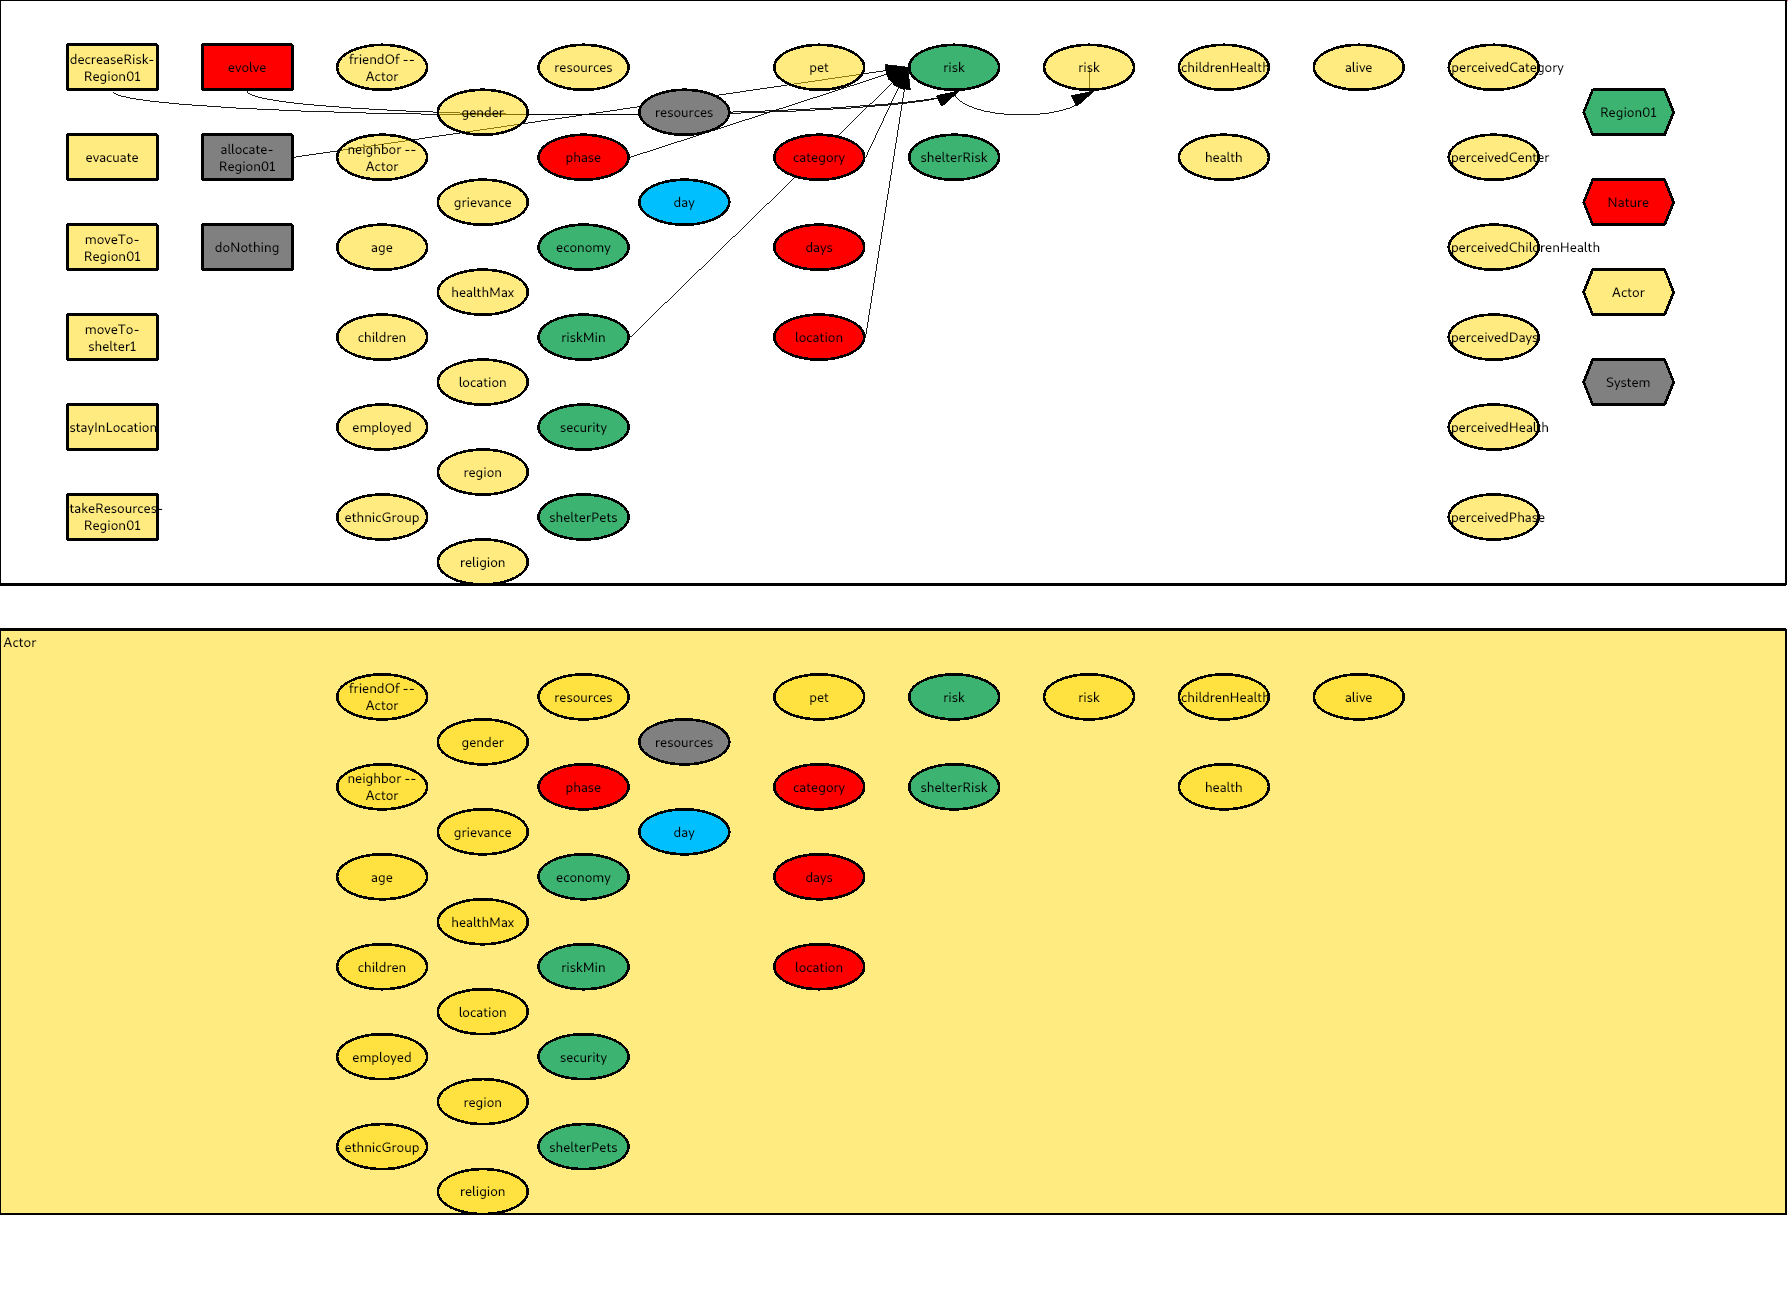
\includegraphics[width=\textwidth]{images/riskOfRegion01.png}%
\begin{flushleft}%
\verb|psychsim/domains/groundtruth/simulation/region.py:51|%
\end{flushleft}%
\subsubsection{Effect of Actor{-}decreaseRisk{-}Region01 on Region01's risk}%
\label{ssubsec:Effect of Actor{-}decreaseRisk{-}Region01 on Region01's risk}%
\begin{flushleft}%
\verb|psychsim/domains/groundtruth/simulation/actor.py:554|%
\linebreak%
$\mbox{\textbf{Region01's risk}} '$%
$\leftarrow$%
80\%%
$\cdot$%
\textbf{Region01's risk}%
+%
20\%%
$\cdot$%
\textbf{Region01's riskMin}%
\end{flushleft}

%
\subsubsection{Effect of Nature{-}evolve on Region01's risk}%
\label{ssubsec:Effect of Nature{-}evolve on Region01's risk}%
\begin{flushleft}%
\verb|psychsim/domains/groundtruth/simulation/nature.py:132|%
\linebreak%
IF %
$\mbox{\textbf{Nature's phase}} '$%
$=$%
\textbf{active}%
\linebreak%
\hspace*{2em}%
THEN %
: %
IF %
$\mbox{\textbf{Nature's location}} '$%
\linebreak%
\hspace*{4em}%
OTHERWISE %
: %
$\mbox{\textbf{Region01's risk}} '$%
$\leftarrow$%
80\%%
$\cdot$%
\textbf{Region01's risk}%
+%
20\%%
$\cdot$%
\textbf{Region01's riskMin}%
\linebreak%
\hspace*{4em}%
$= \mbox{\textbf{Region01}}$%
: %
IF %
\textbf{Nature's category}%
\linebreak%
\hspace*{6em}%
$= \mbox{\textbf{1}}$%
: %
$\mbox{\textbf{Region01's risk}} '$%
$\leftarrow$%
80\%%
$\cdot$%
\textbf{Region01's risk}%
+0.20%
\linebreak%
\hspace*{6em}%
$= \mbox{\textbf{2}}$%
: %
$\mbox{\textbf{Region01's risk}} '$%
$\leftarrow$%
60\%%
$\cdot$%
\textbf{Region01's risk}%
+0.40%
\linebreak%
\hspace*{6em}%
$= \mbox{\textbf{3}}$%
: %
$\mbox{\textbf{Region01's risk}} '$%
$\leftarrow$%
39\%%
$\cdot$%
\textbf{Region01's risk}%
+0.60%
\linebreak%
\hspace*{6em}%
$= \mbox{\textbf{4}}$%
: %
$\mbox{\textbf{Region01's risk}} '$%
$\leftarrow$%
19\%%
$\cdot$%
\textbf{Region01's risk}%
+0.80%
\linebreak%
\hspace*{6em}%
$= \mbox{\textbf{5}}$%
: %
$\mbox{\textbf{Region01's risk}} '$%
$\leftarrow$%
0\%%
$\cdot$%
\textbf{Region01's risk}%
+1.00%
\linebreak%
\hspace*{2em}%
ELSE %
: %
$\mbox{\textbf{Region01's risk}} '$%
$\leftarrow$%
80\%%
$\cdot$%
\textbf{Region01's risk}%
+%
20\%%
$\cdot$%
\textbf{Region01's riskMin}%
\end{flushleft}

%
\subsubsection{Effect of System{-}allocate{-}Region01 on Region01's risk}%
\label{ssubsec:Effect of System{-}allocate{-}Region01 on Region01's risk}%
\begin{flushleft}%
\verb|psychsim/domains/groundtruth/simulation/system.py:42|%
\linebreak%
$\mbox{\textbf{Region01's risk}} '$%
$\leftarrow$%
80\%%
$\cdot$%
\textbf{Region01's risk}%
\end{flushleft}

%
\subsection{Region01's riskMin}%
\label{subsec:Region01's riskMin}%
Minimum level of risk in this region%
\begin{description}%
\item[Type:]%
Real%
\end{description}%
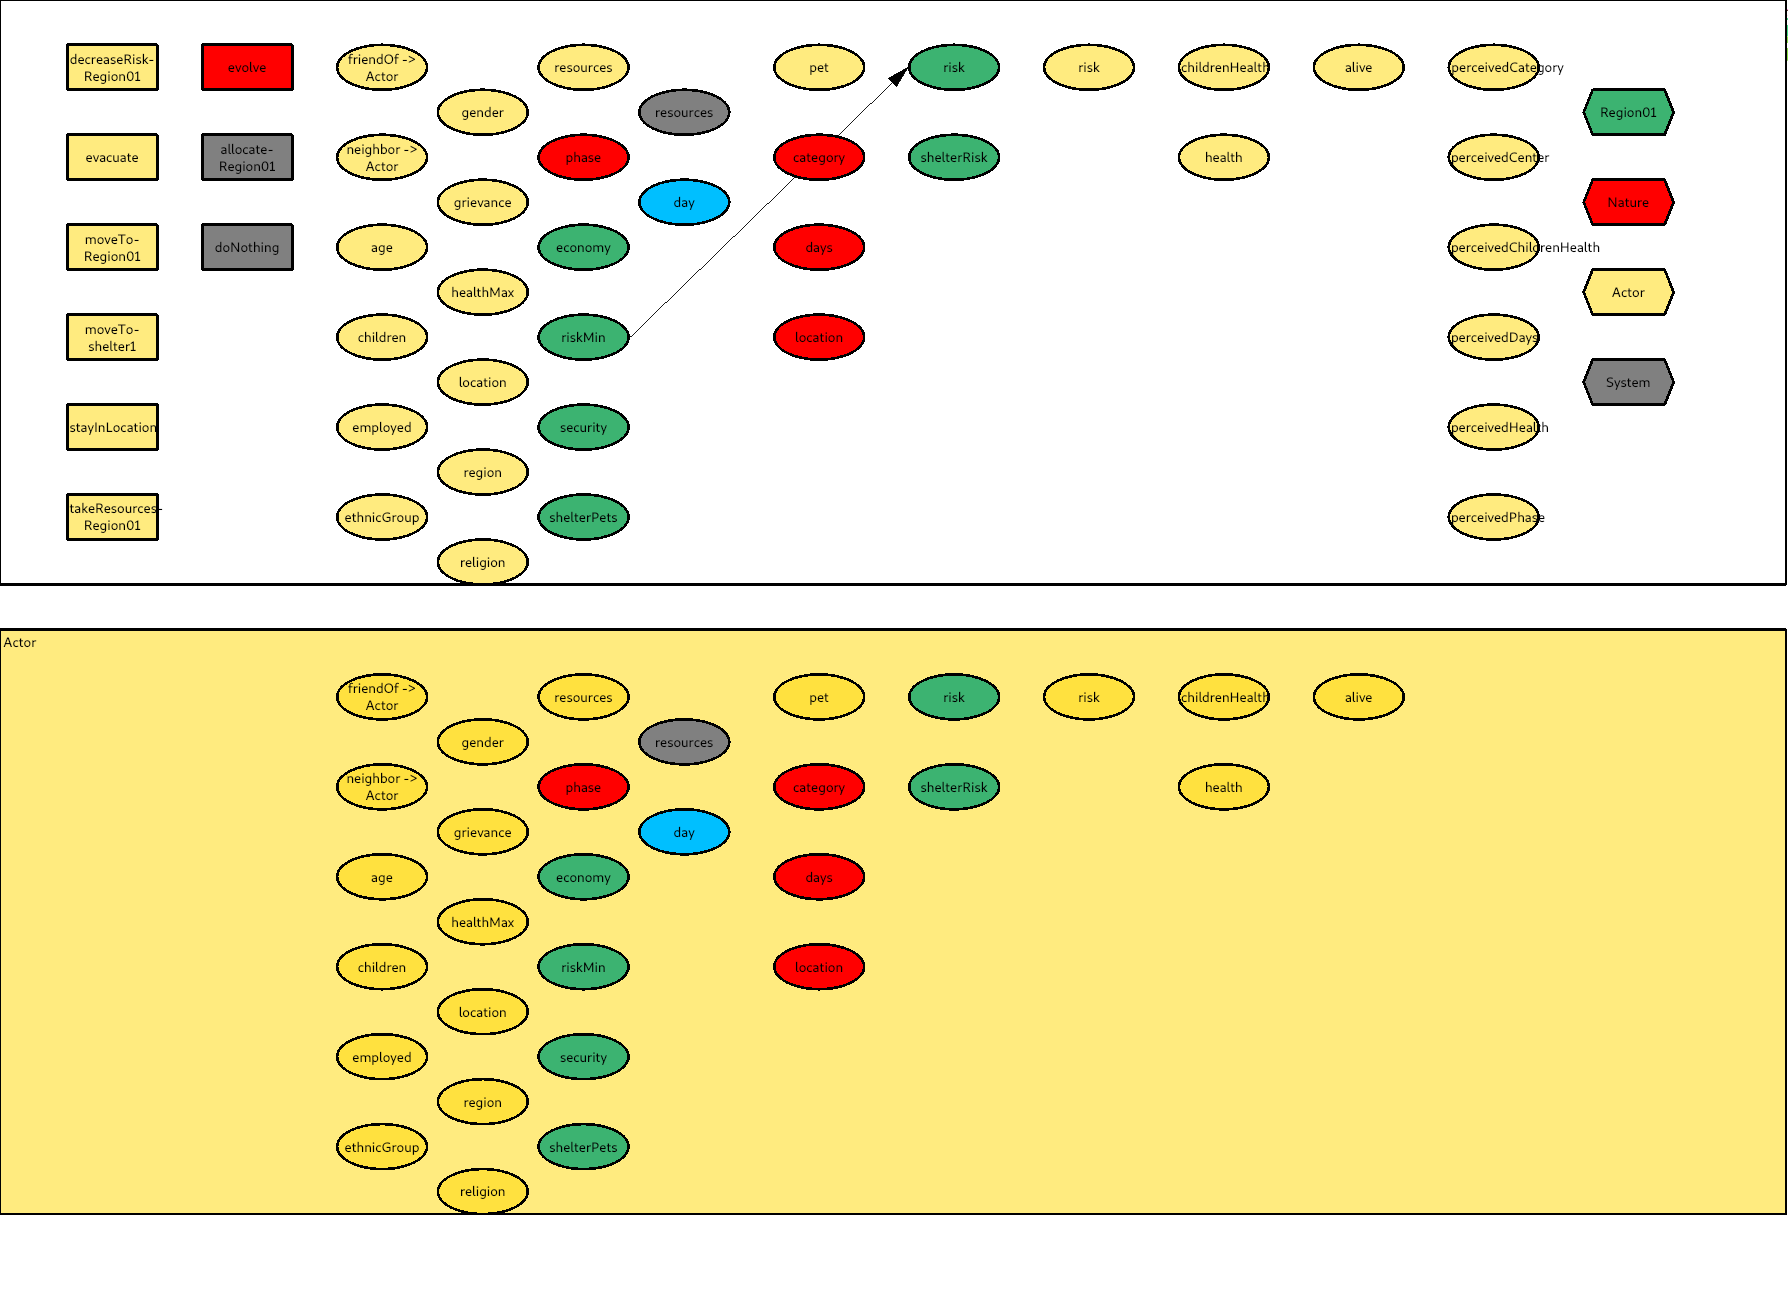
\includegraphics[width=\textwidth]{images/riskMinOfRegion01.png}%
\begin{flushleft}%
\verb|psychsim/domains/groundtruth/simulation/region.py:66|%
\end{flushleft}

%
\subsection{Region01's security}%
\label{subsec:Region01's security}%
Level of law enforcement in region%
\begin{description}%
\item[Type:]%
Real%
\end{description}%
\begin{flushleft}%
\verb|psychsim/domains/groundtruth/simulation/region.py:70|%
\end{flushleft}

%
\subsection{Region01's shelterPets}%
\label{subsec:Region01's shelterPets}%
\begin{description}%
\item[Type:]%
Boolean%
\end{description}%
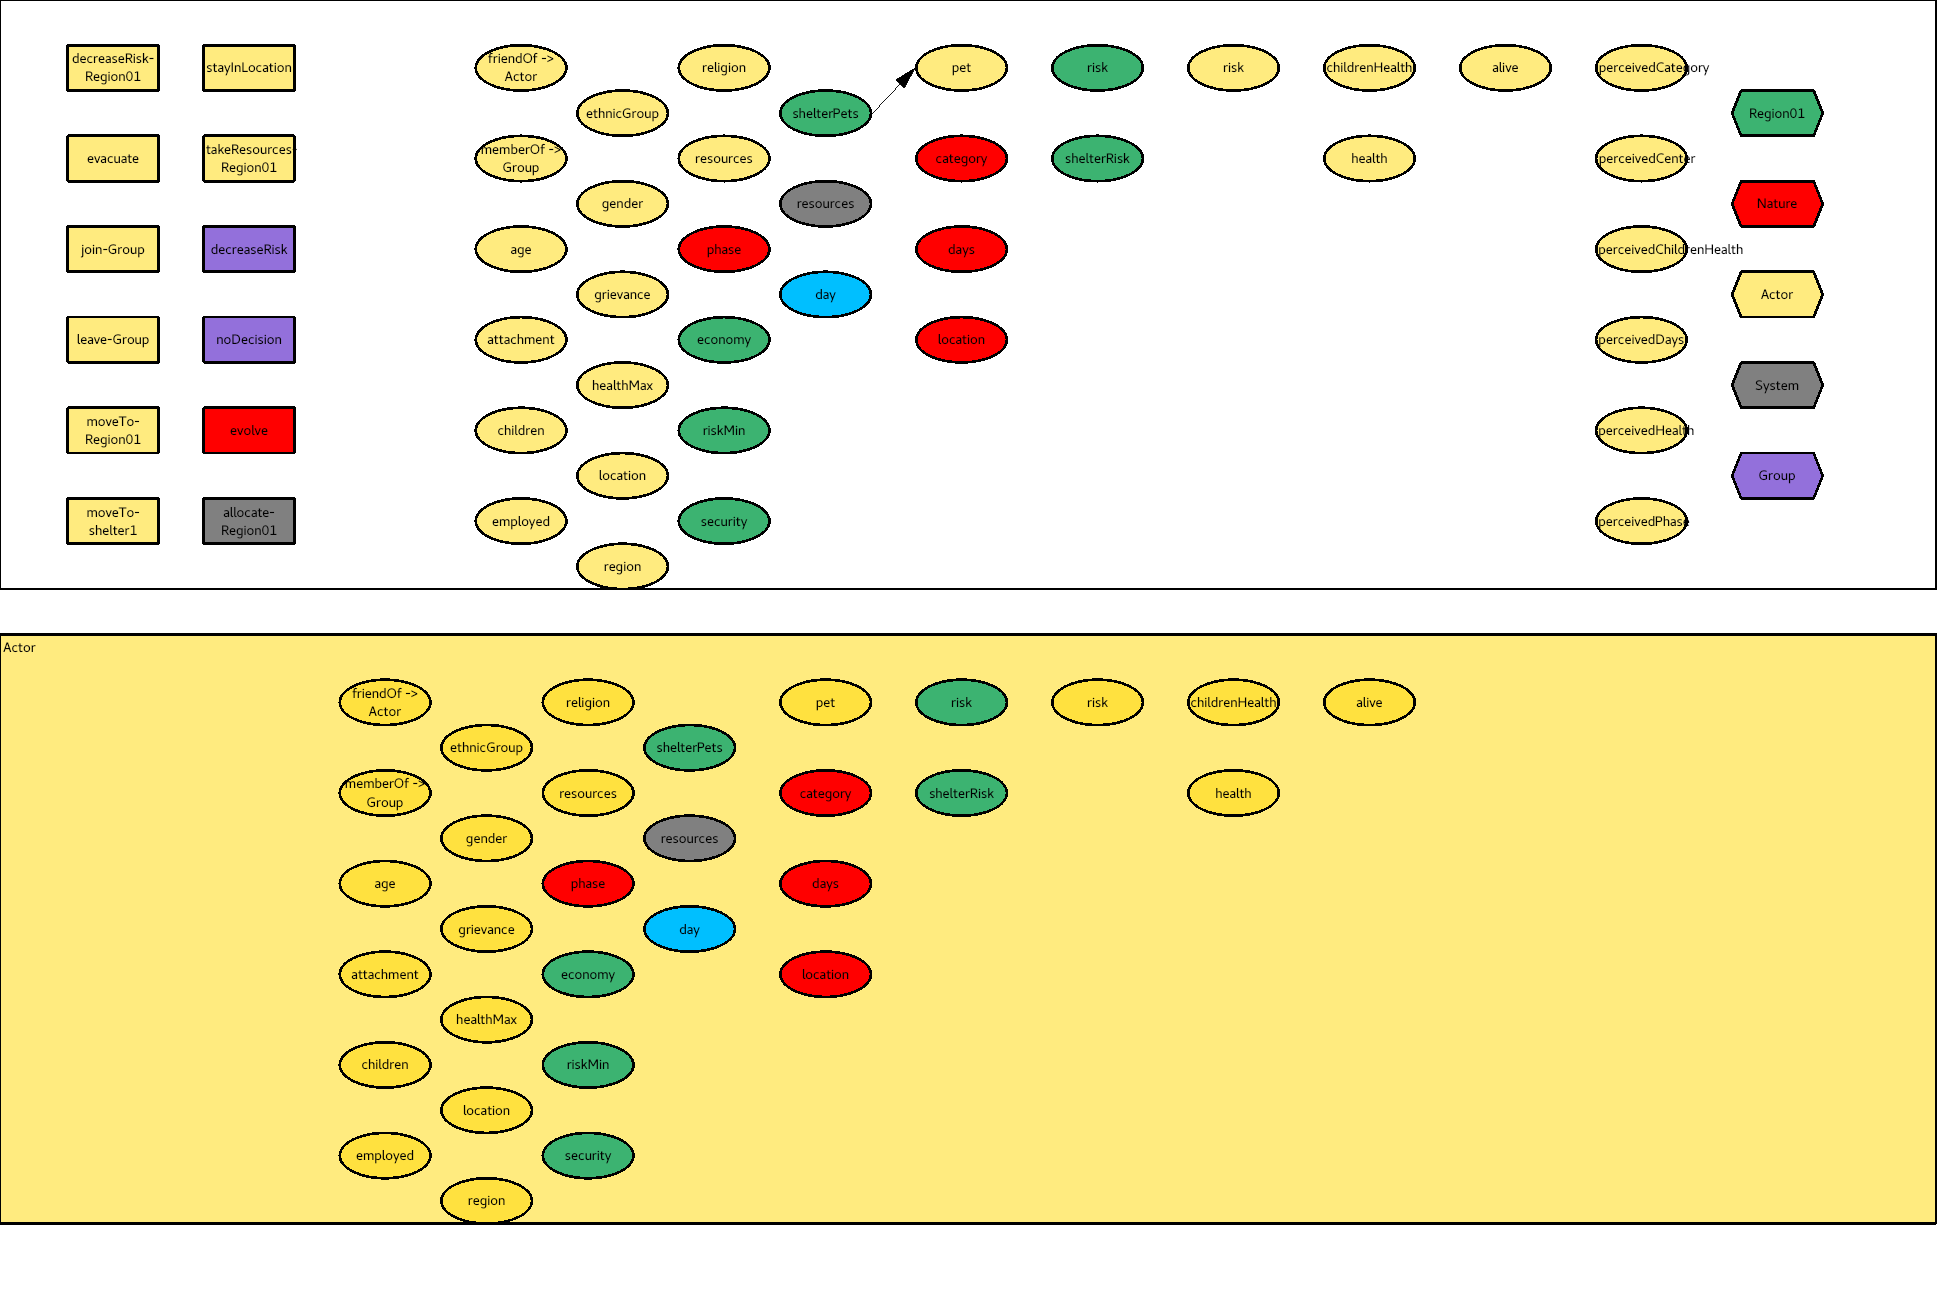
\includegraphics[width=\textwidth]{images/shelterPetsOfRegion01.png}%
\begin{flushleft}%
\verb|psychsim/domains/groundtruth/simulation/region.py:94|%
\end{flushleft}

%
\subsection{Region01's shelterRisk}%
\label{subsec:Region01's shelterRisk}%
\begin{description}%
\item[Type:]%
Real%
\end{description}%
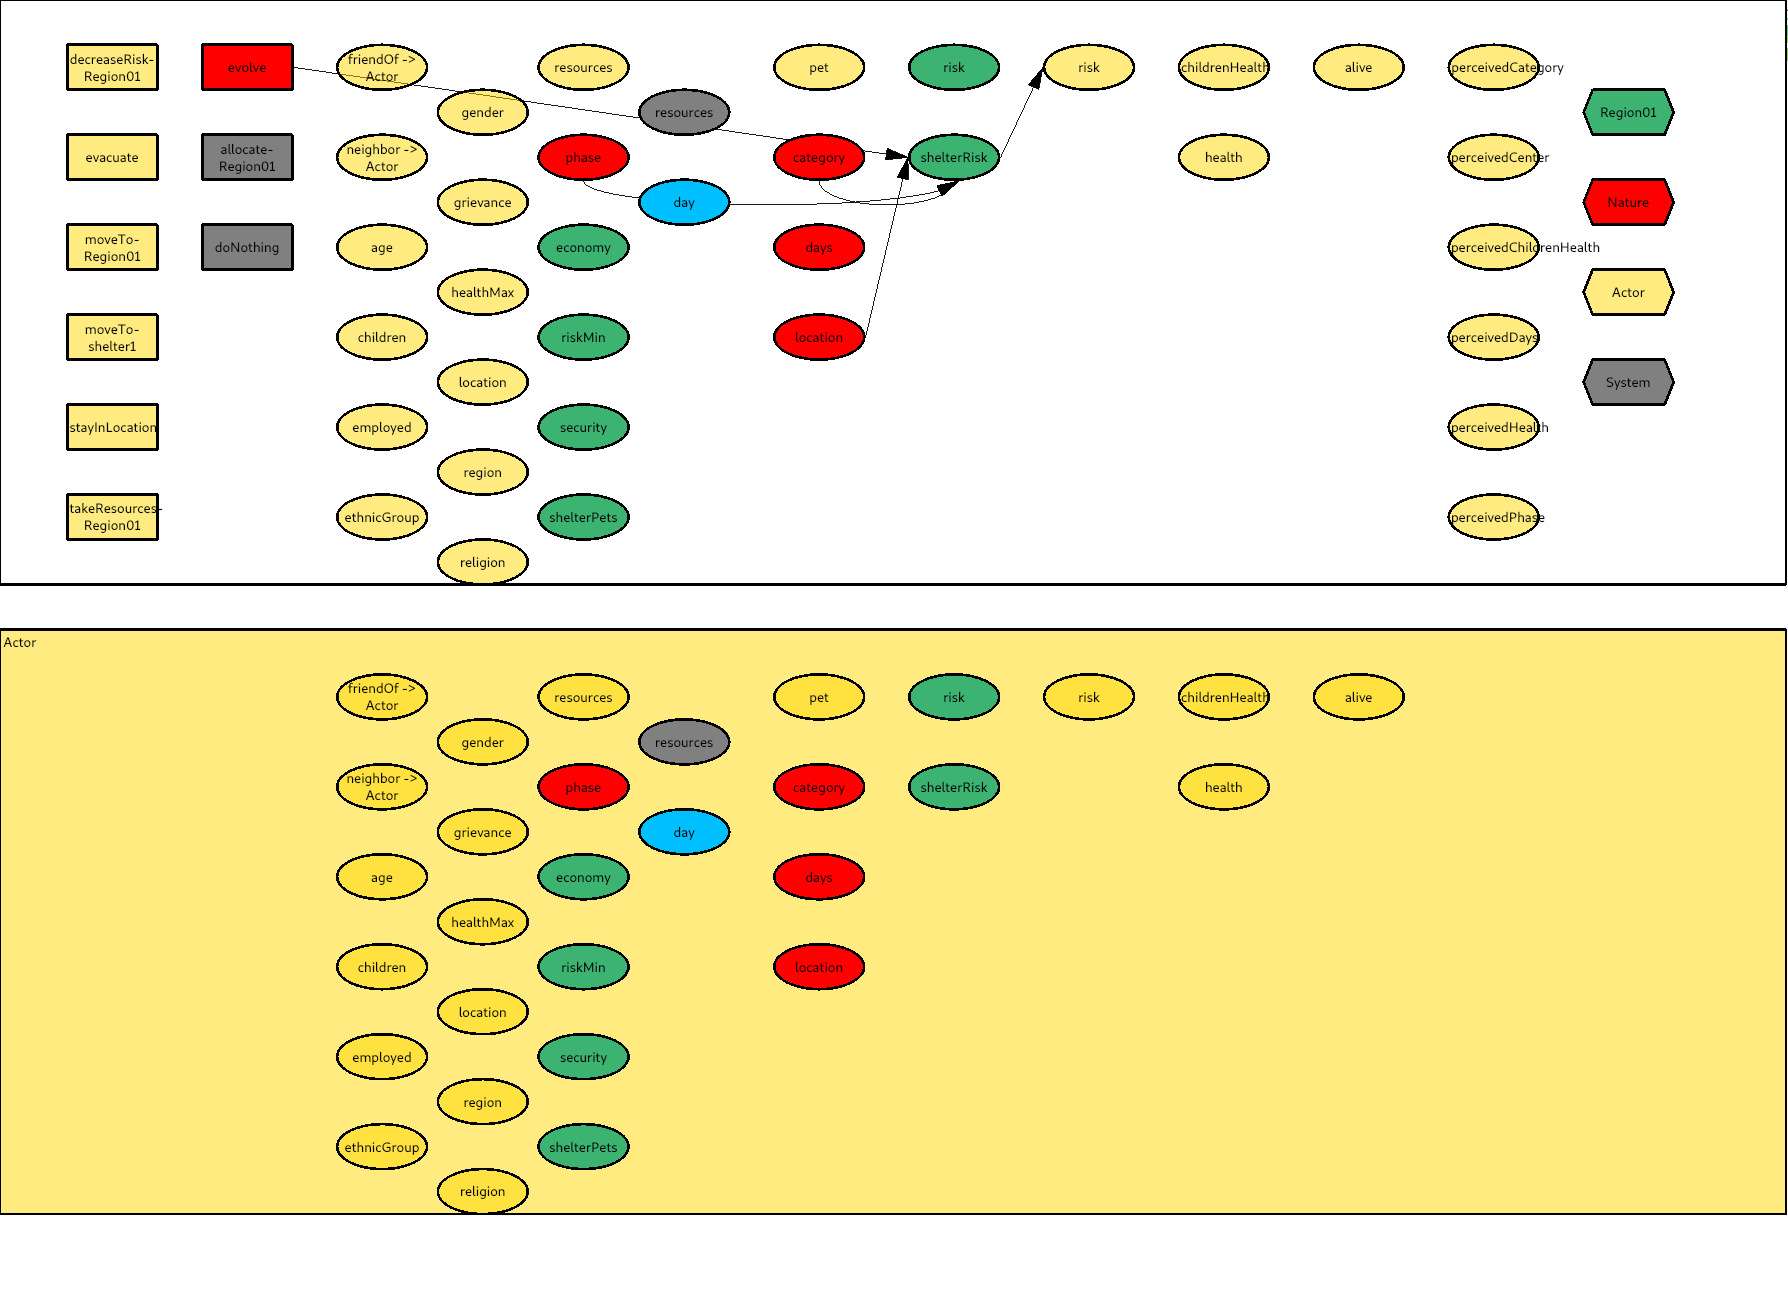
\includegraphics[width=\textwidth]{images/shelterRiskOfRegion01.png}%
\begin{flushleft}%
\verb|psychsim/domains/groundtruth/simulation/region.py:88|%
\end{flushleft}%
\subsubsection{Effect of Nature{-}evolve on Region01's shelterRisk}%
\label{ssubsec:Effect of Nature{-}evolve on Region01's shelterRisk}%
\begin{flushleft}%
\verb|psychsim/domains/groundtruth/simulation/nature.py:147|%
\linebreak%
IF %
$\mbox{\textbf{Nature's phase}} '$%
$=$%
\textbf{active}%
\linebreak%
\hspace*{2em}%
THEN %
: %
IF %
$\mbox{\textbf{Nature's location}} '$%
$=$%
\textbf{Region01}%
\linebreak%
\hspace*{4em}%
THEN %
: %
IF %
\textbf{Nature's category}%
\linebreak%
\hspace*{6em}%
$= \mbox{\textbf{1}}$%
: %
$\mbox{\textbf{Region01's shelterRisk}} '$%
$\leftarrow$%
80\%%
$\cdot$%
\textbf{Region01's shelterRisk}%
+0.20%
\linebreak%
\hspace*{6em}%
$= \mbox{\textbf{2}}$%
: %
$\mbox{\textbf{Region01's shelterRisk}} '$%
$\leftarrow$%
80\%%
$\cdot$%
\textbf{Region01's shelterRisk}%
+0.20%
\linebreak%
\hspace*{6em}%
$= \mbox{\textbf{3}}$%
: %
$\mbox{\textbf{Region01's shelterRisk}} '$%
$\leftarrow$%
80\%%
$\cdot$%
\textbf{Region01's shelterRisk}%
+0.20%
\linebreak%
\hspace*{6em}%
$= \mbox{\textbf{4}}$%
: %
$\mbox{\textbf{Region01's shelterRisk}} '$%
$\leftarrow$%
80\%%
$\cdot$%
\textbf{Region01's shelterRisk}%
+0.20%
\linebreak%
\hspace*{6em}%
$= \mbox{\textbf{5}}$%
: %
$\mbox{\textbf{Region01's shelterRisk}} '$%
$\leftarrow$%
80\%%
$\cdot$%
\textbf{Region01's shelterRisk}%
+0.20%
\linebreak%
\hspace*{4em}%
ELSE %
: %
$\mbox{\textbf{Region01's shelterRisk}} '$%
$\leftarrow$%
\textbf{Region01's shelterRisk}%
\linebreak%
\hspace*{2em}%
ELSE %
: %
$\mbox{\textbf{Region01's shelterRisk}} '$%
$\leftarrow$%
80\%%
$\cdot$%
\textbf{Region01's shelterRisk}%
\end{flushleft}

%
\subsection{System's resources}%
\label{subsec:System's resources}%
\begin{description}%
\item[Type:]%
Integer%
\end{description}%
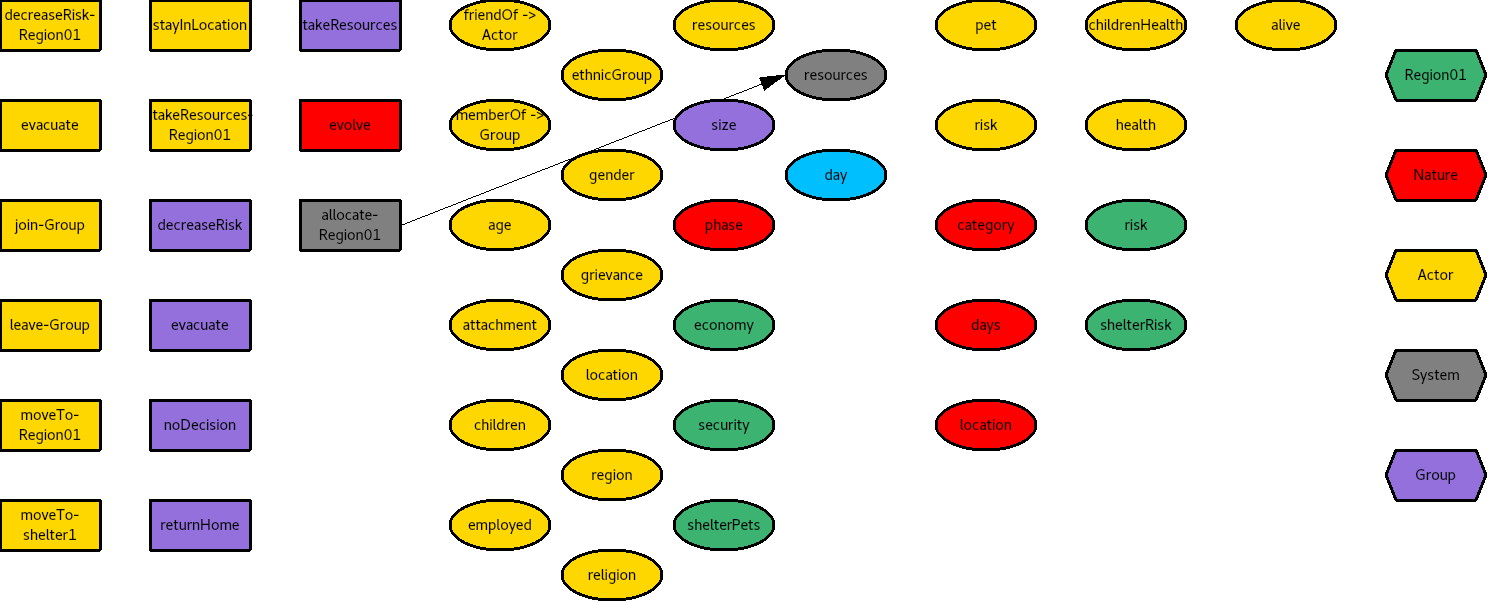
\includegraphics[width=\textwidth]{images/resourcesOfSystem.png}%
\begin{flushleft}%
\verb|psychsim/domains/groundtruth/simulation/system.py:20|%
\end{flushleft}%
\subsubsection{Effect of System{-}allocate{-}Region01 on System's resources}%
\label{ssubsec:Effect of System{-}allocate{-}Region01 on System's resources}%
\begin{flushleft}%
\verb|psychsim/domains/groundtruth/simulation/system.py:44|%
\linebreak%
$\mbox{\textbf{System's resources}} '$%
$\leftarrow$%
\textbf{System's resources}%
\end{flushleft}

%
\subsection{day}%
\label{subsec:day}%
\begin{description}%
\item[Type:]%
Integer%
\end{description}%
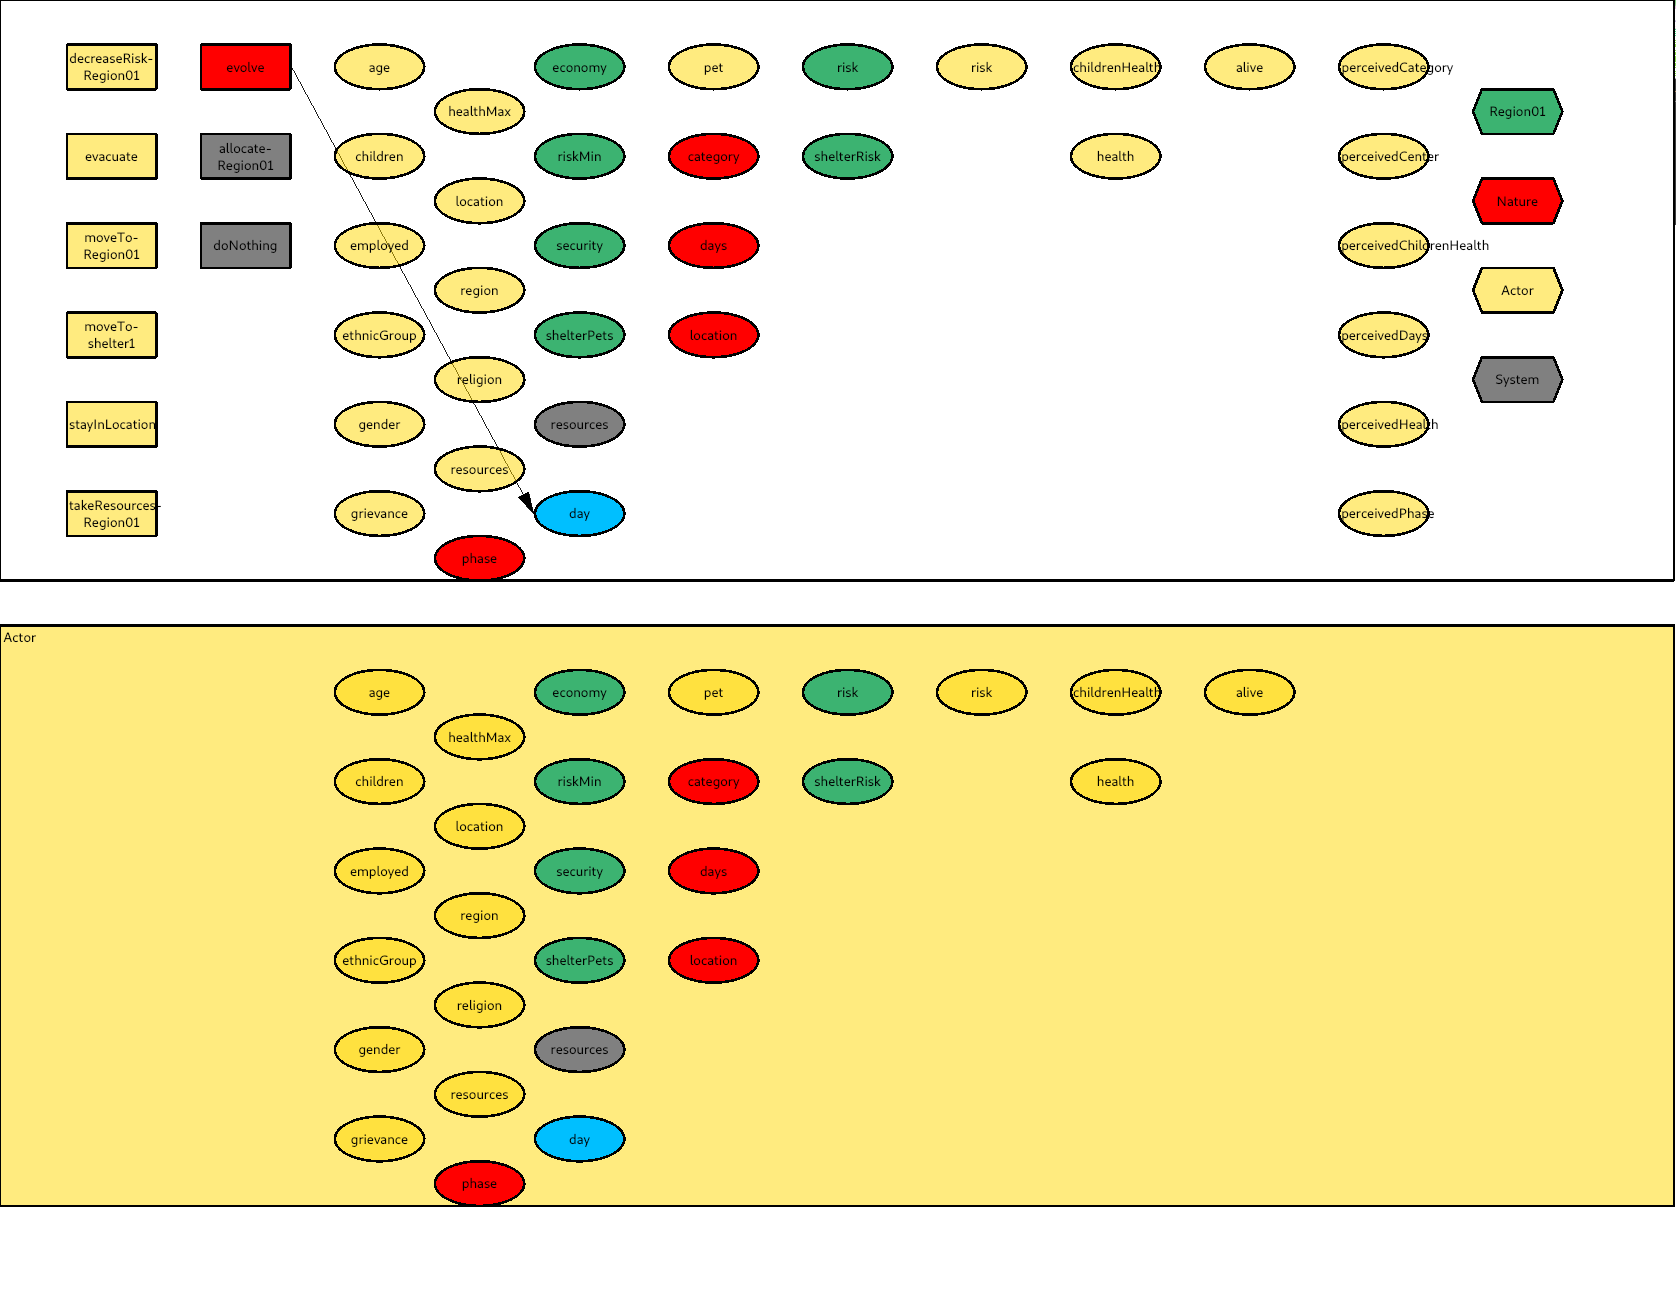
\includegraphics[width=\textwidth]{images/day.png}%
\begin{flushleft}%
\verb|psychsim/domains/groundtruth/simulation/create.py:47|%
\end{flushleft}%
\subsubsection{Effect of Nature{-}evolve on day}%
\label{ssubsec:Effect of Nature{-}evolve on day}%
\begin{flushleft}%
\verb|psychsim/domains/groundtruth/simulation/nature.py:152|%
\linebreak%
$\mbox{\textbf{day}} '$%
$\leftarrow$%
\textbf{day}%
+1%
\end{flushleft}

%
\section{Relations}%
\label{sec:Relations}%
\subsection{Actor friendOf Actor}%
\label{subsec:Actor friendOf Actor}%
\begin{description}%
\item[Type:]%
Boolean%
\end{description}%
\begin{flushleft}%
\verb|psychsim/domains/groundtruth/simulation/actor.py:750|%
\end{flushleft}

%
\subsection{Actor neighbor Actor}%
\label{subsec:Actor neighbor Actor}%
\begin{description}%
\item[Type:]%
Boolean%
\end{description}%
\begin{flushleft}%
\verb|psychsim/domains/groundtruth/simulation/actor.py:827|%
\end{flushleft}

%
\section{Actions}%
\label{sec:Actions}%
\subsection{Nature evolve None}%
\label{subsec:Nature evolve None}%
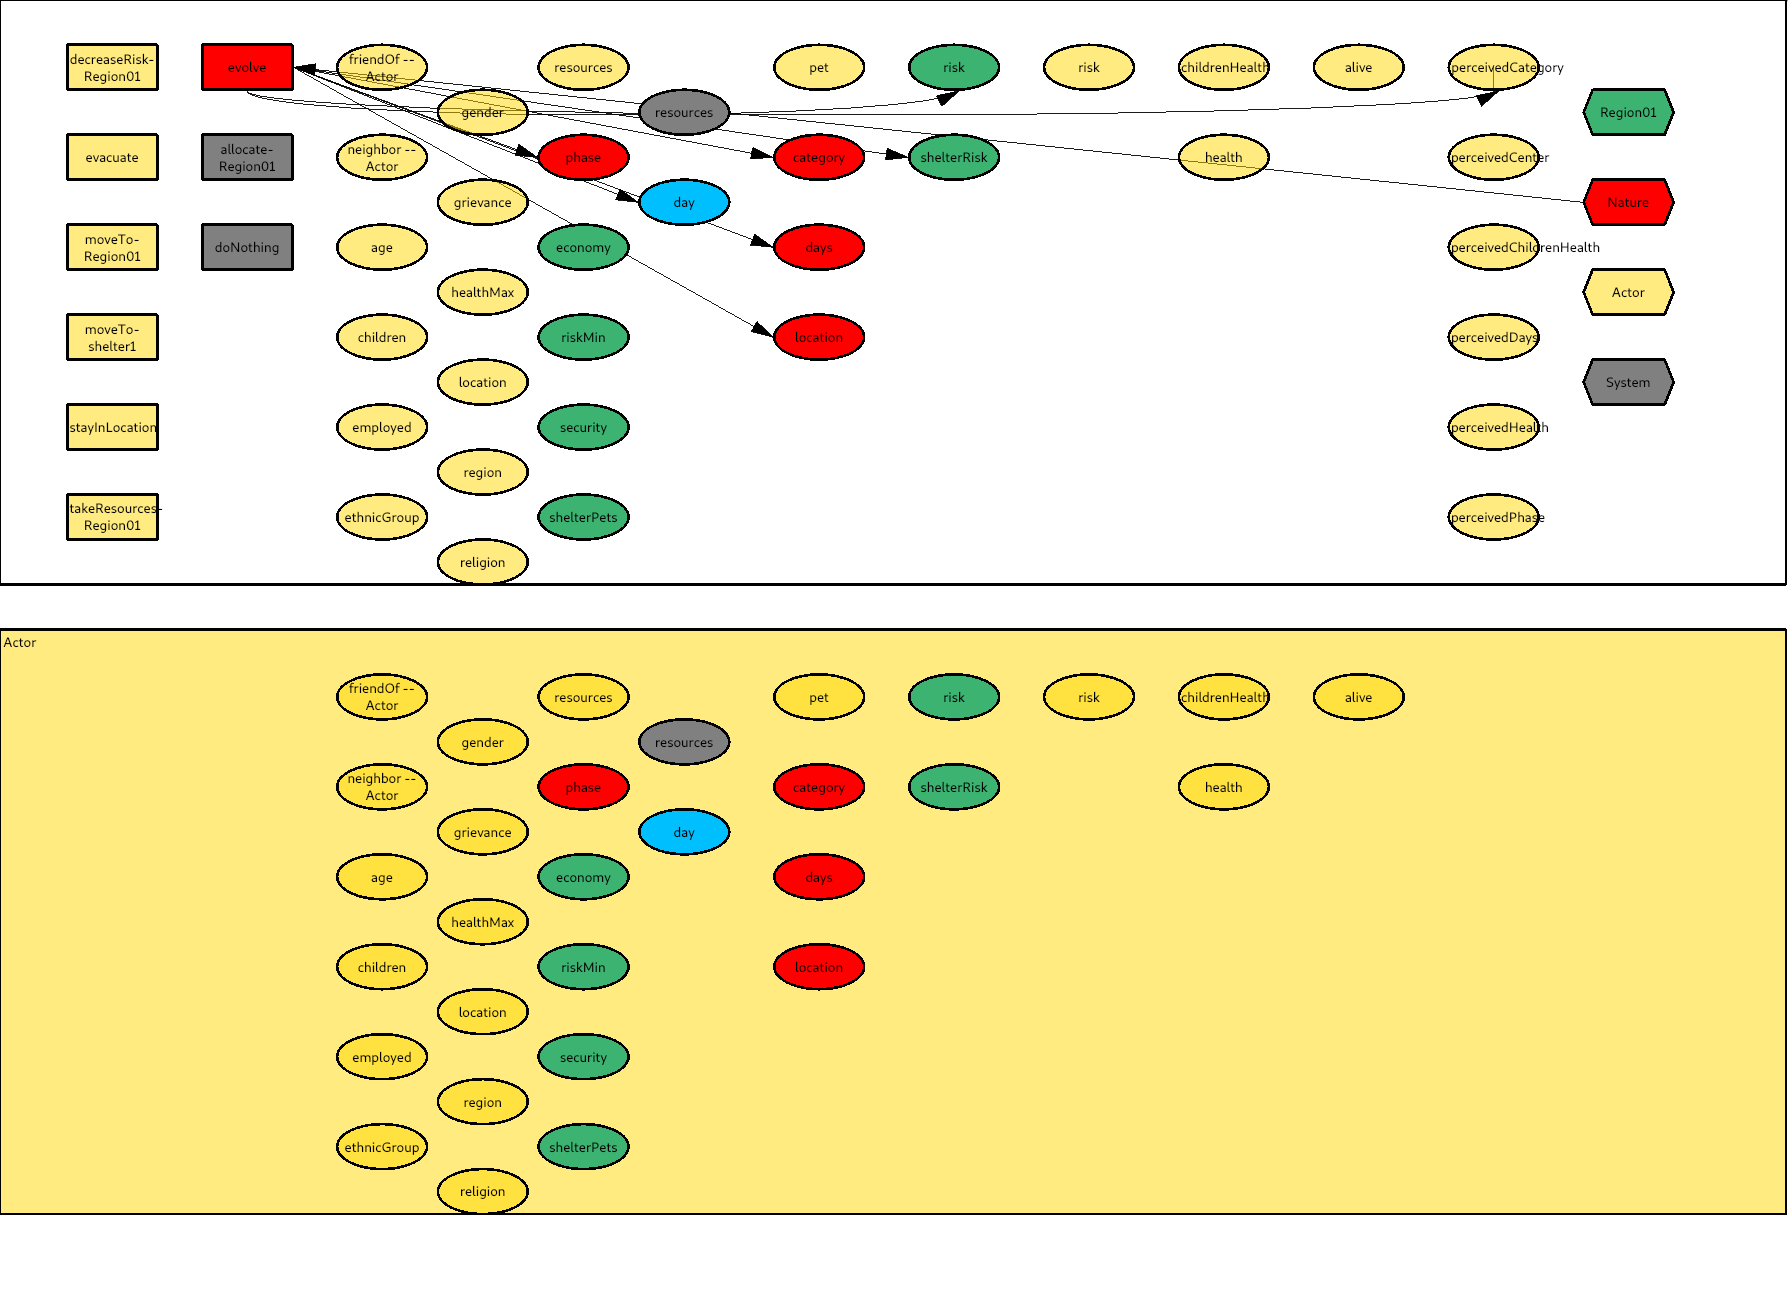
\includegraphics[width=\textwidth]{images/Nature-evolve.png}%
\begin{flushleft}%
\verb|psychsim/domains/groundtruth/simulation/nature.py:14|%
\end{flushleft}%
\subsubsection{Effect on Nature's category of Nature evolve None}%
\label{ssubsec:Effect on Nature's category of Nature evolve None}%
\begin{flushleft}%
IF %
$\mbox{\textbf{Nature's phase}} '$%
\linebreak%
\hspace*{2em}%
$= \mbox{\textbf{approaching}}$%
: %
IF %
\textbf{Nature's category}%
$=$%
0%
\linebreak%
\hspace*{4em}%
THEN %
: %
\linebreak%
\hspace*{6em}%
20\%%
: %
$\mbox{\textbf{Nature's category}} '$%
$\leftarrow$%
1%
\linebreak%
\hspace*{6em}%
20\%%
: %
$\mbox{\textbf{Nature's category}} '$%
$\leftarrow$%
2%
\linebreak%
\hspace*{6em}%
20\%%
: %
$\mbox{\textbf{Nature's category}} '$%
$\leftarrow$%
3%
\linebreak%
\hspace*{6em}%
20\%%
: %
$\mbox{\textbf{Nature's category}} '$%
$\leftarrow$%
4%
\linebreak%
\hspace*{6em}%
20\%%
: %
$\mbox{\textbf{Nature's category}} '$%
$\leftarrow$%
5%
\linebreak%
\hspace*{4em}%
ELSE %
: %
IF %
\textbf{Nature's category}%
$=$%
1%
\linebreak%
\hspace*{6em}%
THEN %
: %
\linebreak%
\hspace*{8em}%
60\%%
: %
$\mbox{\textbf{Nature's category}} '$%
$\leftarrow$%
\textbf{Nature's category}%
\linebreak%
\hspace*{8em}%
40\%%
: %
$\mbox{\textbf{Nature's category}} '$%
$\leftarrow$%
2%
\linebreak%
\hspace*{6em}%
ELSE %
: %
IF %
\textbf{Nature's category}%
$=$%
5%
\linebreak%
\hspace*{8em}%
THEN %
: %
\linebreak%
\hspace*{10em}%
40\%%
: %
$\mbox{\textbf{Nature's category}} '$%
$\leftarrow$%
4%
\linebreak%
\hspace*{10em}%
60\%%
: %
$\mbox{\textbf{Nature's category}} '$%
$\leftarrow$%
\textbf{Nature's category}%
\linebreak%
\hspace*{8em}%
ELSE %
: %
\linebreak%
\hspace*{10em}%
20\%%
: %
$\mbox{\textbf{Nature's category}} '$%
$\leftarrow$%
\textbf{Nature's category}%
${-}1$%
\linebreak%
\hspace*{10em}%
60\%%
: %
$\mbox{\textbf{Nature's category}} '$%
$\leftarrow$%
\textbf{Nature's category}%
\linebreak%
\hspace*{10em}%
20\%%
: %
$\mbox{\textbf{Nature's category}} '$%
$\leftarrow$%
\textbf{Nature's category}%
+1%
\linebreak%
\hspace*{2em}%
$= \mbox{\textbf{active}}$%
: %
$\mbox{\textbf{Nature's category}} '$%
$\leftarrow$%
\textbf{Nature's category}%
\linebreak%
\hspace*{2em}%
$= \mbox{\textbf{none}}$%
: %
$\mbox{\textbf{Nature's category}} '$%
$\leftarrow$%
0%
\end{flushleft}

%
\subsubsection{Effect on Nature's days of Nature evolve None}%
\label{ssubsec:Effect on Nature's days of Nature evolve None}%
\begin{flushleft}%
IF %
\textbf{Nature's phase}%
$=$%
$\mbox{\textbf{Nature's phase}} '$%
\linebreak%
\hspace*{2em}%
THEN %
: %
$\mbox{\textbf{Nature's days}} '$%
$\leftarrow$%
\textbf{Nature's days}%
+1%
\linebreak%
\hspace*{2em}%
ELSE %
: %
$\mbox{\textbf{Nature's days}} '$%
$\leftarrow$%
0%
\end{flushleft}

%
\subsubsection{Effect on Nature's location of Nature evolve None}%
\label{ssubsec:Effect on Nature's location of Nature evolve None}%
\begin{flushleft}%
IF %
$\mbox{\textbf{Nature's phase}} '$%
\linebreak%
\hspace*{2em}%
$= \mbox{\textbf{approaching}}$%
: %
IF %
\textbf{Nature's location}%
$=$%
\textbf{none}%
\linebreak%
\hspace*{4em}%
THEN %
: %
$\mbox{\textbf{Nature's location}} '$%
$\leftarrow$%
\textbf{Region01}%
\linebreak%
\hspace*{4em}%
ELSE %
: %
$\mbox{\textbf{Nature's location}} '$%
$\leftarrow$%
\textbf{Nature's location}%
\linebreak%
\hspace*{2em}%
$= \mbox{\textbf{active}}$%
: %
IF %
\textbf{Nature's phase}%
$=$%
\textbf{approaching}%
\linebreak%
\hspace*{4em}%
THEN %
: %
$\mbox{\textbf{Nature's location}} '$%
$\leftarrow$%
\textbf{Nature's location}%
\linebreak%
\hspace*{4em}%
ELSE %
: %
IF %
\textbf{Nature's location}%
\linebreak%
\hspace*{6em}%
OTHERWISE %
: %
$\mbox{\textbf{Nature's location}} '$%
$\leftarrow$%
\textbf{Nature's location}%
\linebreak%
\hspace*{6em}%
$= \mbox{\textbf{Region01}}$%
: %
\linebreak%
\hspace*{8em}%
20\%%
: %
$\mbox{\textbf{Nature's location}} '$%
$\leftarrow$%
\textbf{Region01}%
\linebreak%
\hspace*{8em}%
48\%%
: %
$\mbox{\textbf{Nature's location}} '$%
$\leftarrow$%
\textbf{none}%
\linebreak%
\hspace*{2em}%
$= \mbox{\textbf{none}}$%
: %
$\mbox{\textbf{Nature's location}} '$%
$\leftarrow$%
\textbf{none}%
\end{flushleft}

%
\subsubsection{Effect on Nature's phase of Nature evolve None}%
\label{ssubsec:Effect on Nature's phase of Nature evolve None}%
\begin{flushleft}%
IF %
\textbf{Nature's phase}%
\linebreak%
\hspace*{2em}%
$= \mbox{\textbf{none}}$%
: %
IF %
\textbf{Nature's days}%
$>$%
2%
\linebreak%
\hspace*{4em}%
THEN %
: %
\linebreak%
\hspace*{6em}%
60\%%
: %
$\mbox{\textbf{Nature's phase}} '$%
$\leftarrow$%
\textbf{approaching}%
\linebreak%
\hspace*{6em}%
40\%%
: %
$\mbox{\textbf{Nature's phase}} '$%
$\leftarrow$%
\textbf{none}%
\linebreak%
\hspace*{4em}%
ELSE %
: %
$\mbox{\textbf{Nature's phase}} '$%
$\leftarrow$%
\textbf{none}%
\linebreak%
\hspace*{2em}%
$= \mbox{\textbf{approaching}}$%
: %
IF %
\textbf{Nature's days}%
$>$%
2%
\linebreak%
\hspace*{4em}%
THEN %
: %
\linebreak%
\hspace*{6em}%
60\%%
: %
$\mbox{\textbf{Nature's phase}} '$%
$\leftarrow$%
\textbf{active}%
\linebreak%
\hspace*{6em}%
40\%%
: %
$\mbox{\textbf{Nature's phase}} '$%
$\leftarrow$%
\textbf{approaching}%
\linebreak%
\hspace*{4em}%
ELSE %
: %
$\mbox{\textbf{Nature's phase}} '$%
$\leftarrow$%
\textbf{approaching}%
\linebreak%
\hspace*{2em}%
OTHERWISE %
: %
IF %
\textbf{Nature's location}%
$=$%
\textbf{none}%
\linebreak%
\hspace*{4em}%
THEN %
: %
$\mbox{\textbf{Nature's phase}} '$%
$\leftarrow$%
\textbf{none}%
\linebreak%
\hspace*{4em}%
ELSE %
: %
$\mbox{\textbf{Nature's phase}} '$%
$\leftarrow$%
\textbf{active}%
\end{flushleft}

%
\subsubsection{Effect on Region01's risk of Nature evolve None}%
\label{ssubsec:Effect on Region01's risk of Nature evolve None}%
\begin{flushleft}%
IF %
$\mbox{\textbf{Nature's phase}} '$%
$=$%
\textbf{active}%
\linebreak%
\hspace*{2em}%
THEN %
: %
IF %
$\mbox{\textbf{Nature's location}} '$%
\linebreak%
\hspace*{4em}%
OTHERWISE %
: %
$\mbox{\textbf{Region01's risk}} '$%
$\leftarrow$%
80\%%
$\cdot$%
\textbf{Region01's risk}%
+%
20\%%
$\cdot$%
\textbf{Region01's riskMin}%
\linebreak%
\hspace*{4em}%
$= \mbox{\textbf{Region01}}$%
: %
IF %
\textbf{Nature's category}%
\linebreak%
\hspace*{6em}%
$= \mbox{\textbf{1}}$%
: %
$\mbox{\textbf{Region01's risk}} '$%
$\leftarrow$%
80\%%
$\cdot$%
\textbf{Region01's risk}%
+0.20%
\linebreak%
\hspace*{6em}%
$= \mbox{\textbf{2}}$%
: %
$\mbox{\textbf{Region01's risk}} '$%
$\leftarrow$%
60\%%
$\cdot$%
\textbf{Region01's risk}%
+0.40%
\linebreak%
\hspace*{6em}%
$= \mbox{\textbf{3}}$%
: %
$\mbox{\textbf{Region01's risk}} '$%
$\leftarrow$%
39\%%
$\cdot$%
\textbf{Region01's risk}%
+0.60%
\linebreak%
\hspace*{6em}%
$= \mbox{\textbf{4}}$%
: %
$\mbox{\textbf{Region01's risk}} '$%
$\leftarrow$%
19\%%
$\cdot$%
\textbf{Region01's risk}%
+0.80%
\linebreak%
\hspace*{6em}%
$= \mbox{\textbf{5}}$%
: %
$\mbox{\textbf{Region01's risk}} '$%
$\leftarrow$%
0\%%
$\cdot$%
\textbf{Region01's risk}%
+1.00%
\linebreak%
\hspace*{2em}%
ELSE %
: %
$\mbox{\textbf{Region01's risk}} '$%
$\leftarrow$%
80\%%
$\cdot$%
\textbf{Region01's risk}%
+%
20\%%
$\cdot$%
\textbf{Region01's riskMin}%
\end{flushleft}

%
\subsubsection{Effect on Region01's shelterRisk of Nature evolve None}%
\label{ssubsec:Effect on Region01's shelterRisk of Nature evolve None}%
\begin{flushleft}%
IF %
$\mbox{\textbf{Nature's phase}} '$%
$=$%
\textbf{active}%
\linebreak%
\hspace*{2em}%
THEN %
: %
IF %
$\mbox{\textbf{Nature's location}} '$%
$=$%
\textbf{Region01}%
\linebreak%
\hspace*{4em}%
THEN %
: %
IF %
\textbf{Nature's category}%
\linebreak%
\hspace*{6em}%
$= \mbox{\textbf{1}}$%
: %
$\mbox{\textbf{Region01's shelterRisk}} '$%
$\leftarrow$%
80\%%
$\cdot$%
\textbf{Region01's shelterRisk}%
+0.20%
\linebreak%
\hspace*{6em}%
$= \mbox{\textbf{2}}$%
: %
$\mbox{\textbf{Region01's shelterRisk}} '$%
$\leftarrow$%
80\%%
$\cdot$%
\textbf{Region01's shelterRisk}%
+0.20%
\linebreak%
\hspace*{6em}%
$= \mbox{\textbf{3}}$%
: %
$\mbox{\textbf{Region01's shelterRisk}} '$%
$\leftarrow$%
80\%%
$\cdot$%
\textbf{Region01's shelterRisk}%
+0.20%
\linebreak%
\hspace*{6em}%
$= \mbox{\textbf{4}}$%
: %
$\mbox{\textbf{Region01's shelterRisk}} '$%
$\leftarrow$%
80\%%
$\cdot$%
\textbf{Region01's shelterRisk}%
+0.20%
\linebreak%
\hspace*{6em}%
$= \mbox{\textbf{5}}$%
: %
$\mbox{\textbf{Region01's shelterRisk}} '$%
$\leftarrow$%
80\%%
$\cdot$%
\textbf{Region01's shelterRisk}%
+0.20%
\linebreak%
\hspace*{4em}%
ELSE %
: %
$\mbox{\textbf{Region01's shelterRisk}} '$%
$\leftarrow$%
\textbf{Region01's shelterRisk}%
\linebreak%
\hspace*{2em}%
ELSE %
: %
$\mbox{\textbf{Region01's shelterRisk}} '$%
$\leftarrow$%
80\%%
$\cdot$%
\textbf{Region01's shelterRisk}%
\end{flushleft}

%
\subsubsection{Effect on day of Nature evolve None}%
\label{ssubsec:Effect on day of Nature evolve None}%
\begin{flushleft}%
$\mbox{\textbf{day}} '$%
$\leftarrow$%
\textbf{day}%
+1%
\end{flushleft}

%
\subsection{Actor decreaseRisk Region01}%
\label{subsec:Actor decreaseRisk Region01}%
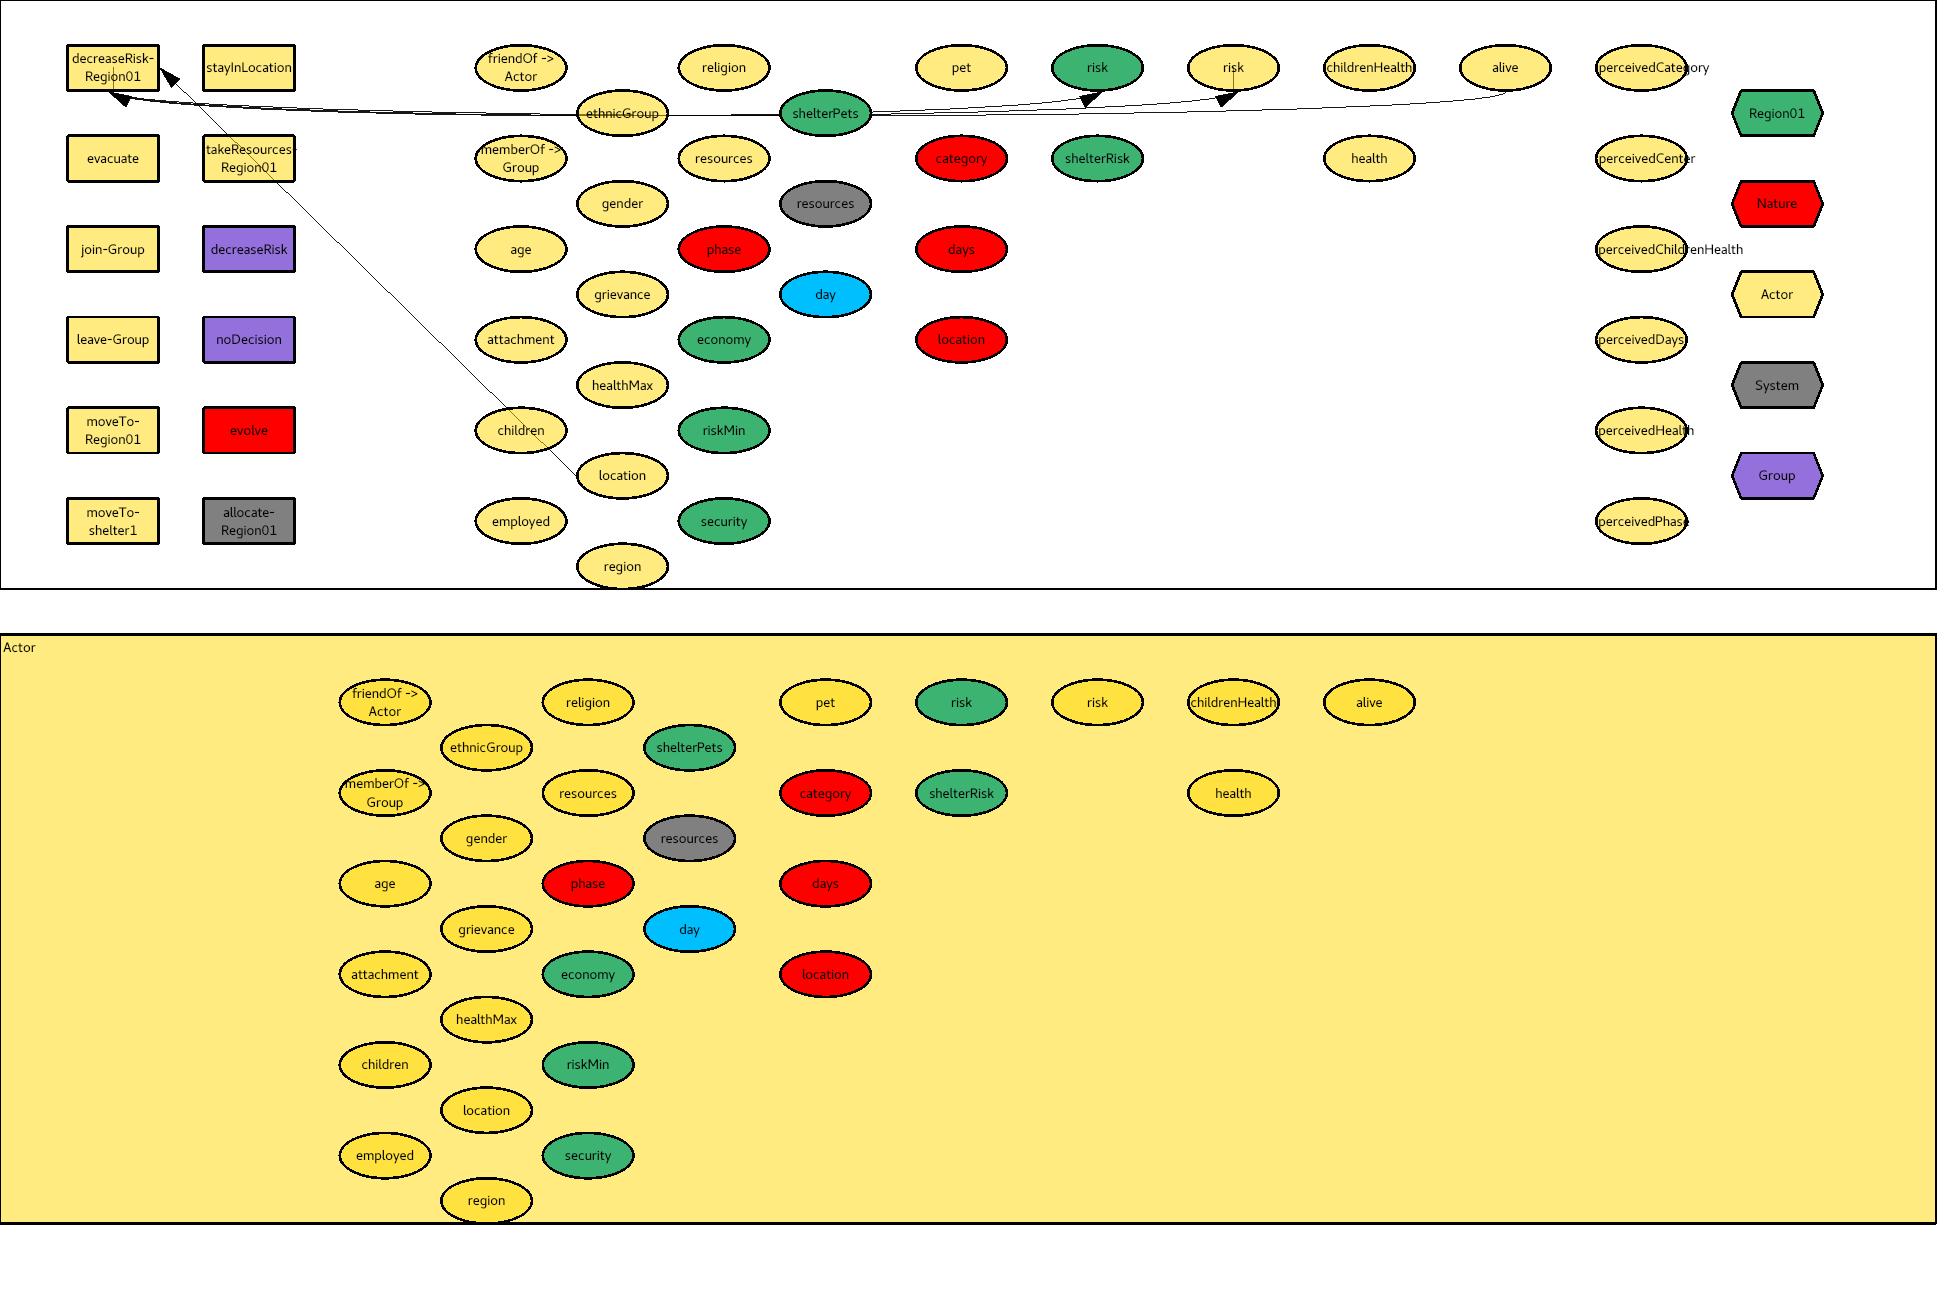
\includegraphics[width=\textwidth]{images/Actor-decreaseRisk-Region01.png}%
\begin{flushleft}%
\verb|psychsim/domains/groundtruth/simulation/actor.py:345|%
\end{flushleft}%
\subsubsection{Applicability of Actor decreaseRisk Region01}%
\label{ssubsec:Applicability of Actor decreaseRisk Region01}%
\begin{flushleft}%
IF %
\textbf{Actor's location}%
$=$%
\textbf{Region01}%
\linebreak%
\hspace*{2em}%
THEN %
: %
IF %
\textbf{Actor's alive}%
\linebreak%
\hspace*{4em}%
THEN %
: %
\textbf{true}%
\linebreak%
\hspace*{4em}%
ELSE %
: %
\textbf{false}%
\linebreak%
\hspace*{2em}%
ELSE %
: %
\textbf{false}%
\end{flushleft}

%
\subsubsection{Effect on Actor's risk of Actor decreaseRisk Region01}%
\label{ssubsec:Effect on Actor's risk of Actor decreaseRisk Region01}%
\begin{flushleft}%
$\mbox{\textbf{Actor's risk}} '$%
$\leftarrow$%
80\%%
$\cdot$%
\textbf{Actor's risk}%
+0.20%
\end{flushleft}

%
\subsubsection{Effect on Region01's risk of Actor decreaseRisk Region01}%
\label{ssubsec:Effect on Region01's risk of Actor decreaseRisk Region01}%
\begin{flushleft}%
$\mbox{\textbf{Region01's risk}} '$%
$\leftarrow$%
80\%%
$\cdot$%
\textbf{Region01's risk}%
+%
20\%%
$\cdot$%
\textbf{Region01's riskMin}%
\end{flushleft}

%
\subsection{Actor evacuate None}%
\label{subsec:Actor evacuate None}%
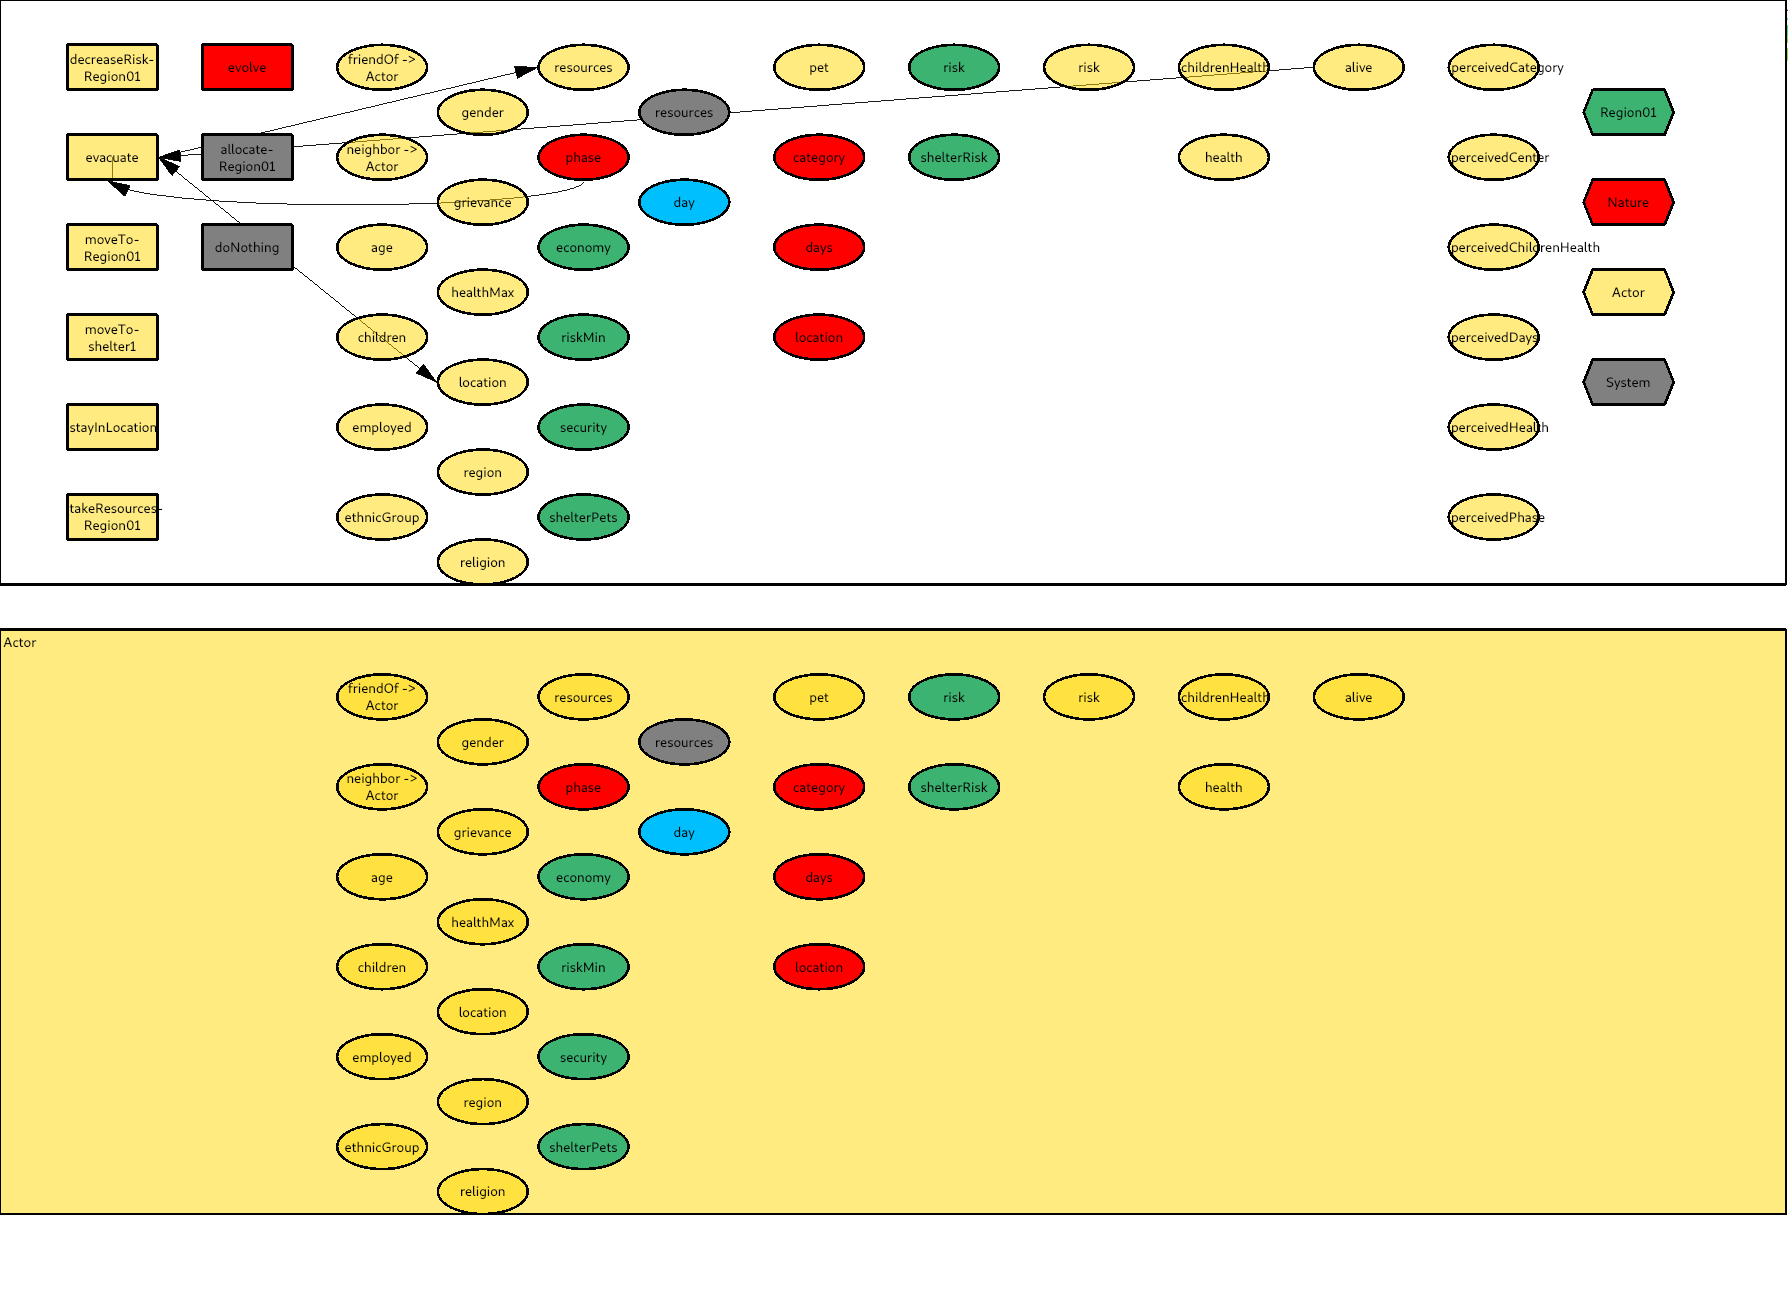
\includegraphics[width=\textwidth]{images/Actor-evacuate.png}%
\begin{flushleft}%
\verb|psychsim/domains/groundtruth/simulation/actor.py:327|%
\end{flushleft}%
\subsubsection{Applicability of Actor evacuate None}%
\label{ssubsec:Applicability of Actor evacuate None}%
\begin{flushleft}%
IF %
\textbf{Nature's phase}%
$=$%
\textbf{none}%
\linebreak%
\hspace*{2em}%
THEN %
: %
\textbf{false}%
\linebreak%
\hspace*{2em}%
ELSE %
: %
IF %
\textbf{Actor's location}%
$=$%
\textbf{evacuated}%
\linebreak%
\hspace*{4em}%
THEN %
: %
\textbf{false}%
\linebreak%
\hspace*{4em}%
ELSE %
: %
IF %
\textbf{Actor's alive}%
\linebreak%
\hspace*{6em}%
THEN %
: %
\textbf{true}%
\linebreak%
\hspace*{6em}%
ELSE %
: %
\textbf{false}%
\end{flushleft}

%
\subsubsection{Effect on Actor's location of Actor evacuate None}%
\label{ssubsec:Effect on Actor's location of Actor evacuate None}%
\begin{flushleft}%
$\mbox{\textbf{Actor's location}} '$%
$\leftarrow$%
\textbf{evacuated}%
\end{flushleft}

%
\subsubsection{Effect on Actor's resources of Actor evacuate None}%
\label{ssubsec:Effect on Actor's resources of Actor evacuate None}%
\begin{flushleft}%
IF %
\textbf{Actor's resources}%
$>$%
0.40%
\linebreak%
\hspace*{2em}%
THEN %
: %
$\mbox{\textbf{Actor's resources}} '$%
$\leftarrow$%
\textbf{Actor's resources}%
${-}0.40$%
\linebreak%
\hspace*{2em}%
ELSE %
: %
$\mbox{\textbf{Actor's resources}} '$%
$\leftarrow$%
0.00%
\end{flushleft}

%
\subsection{Actor moveTo Region01}%
\label{subsec:Actor moveTo Region01}%
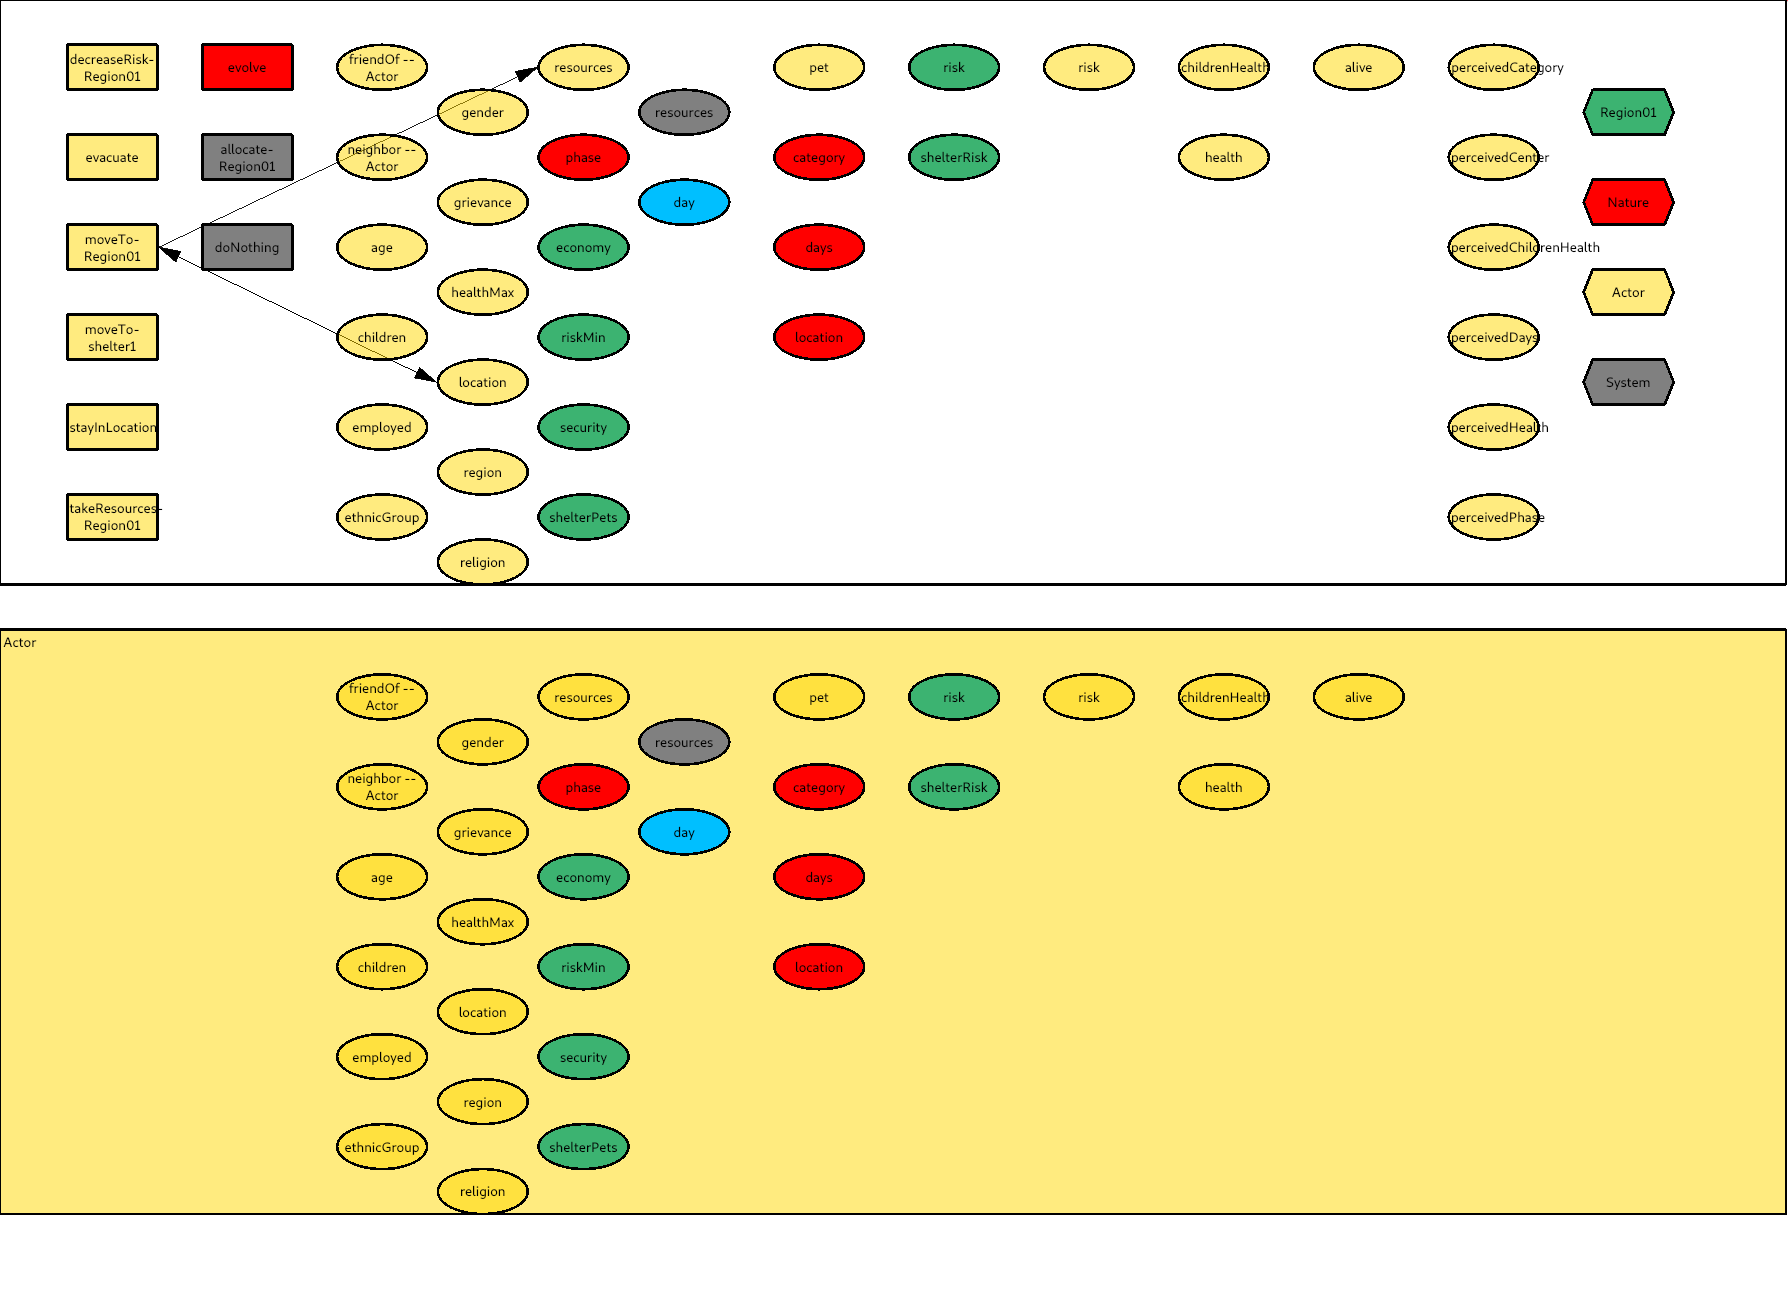
\includegraphics[width=\textwidth]{images/Actor-moveTo-Region01.png}%
\begin{flushleft}%
\verb|psychsim/domains/groundtruth/simulation/actor.py:334|%
\end{flushleft}%
\subsubsection{Applicability of Actor moveTo Region01}%
\label{ssubsec:Applicability of Actor moveTo Region01}%
\begin{flushleft}%
IF %
\textbf{Actor's location}%
$=$%
\textbf{\{'evacuated', 'shelter1'\}}%
\linebreak%
\hspace*{2em}%
THEN %
: %
\textbf{true}%
\linebreak%
\hspace*{2em}%
ELSE %
: %
\textbf{false}%
\end{flushleft}

%
\subsubsection{Effect on Actor's location of Actor moveTo Region01}%
\label{ssubsec:Effect on Actor's location of Actor moveTo Region01}%
\begin{flushleft}%
$\mbox{\textbf{Actor's location}} '$%
$\leftarrow$%
\textbf{Region01}%
\end{flushleft}

%
\subsubsection{Effect on Actor's resources of Actor moveTo Region01}%
\label{ssubsec:Effect on Actor's resources of Actor moveTo Region01}%
\begin{flushleft}%
IF %
\textbf{Actor's alive}%
\linebreak%
\hspace*{2em}%
THEN %
: %
IF %
\textbf{Actor's employed}%
\linebreak%
\hspace*{4em}%
THEN %
: %
$\mbox{\textbf{Actor's resources}} '$%
$\leftarrow$%
60\%%
$\cdot$%
\textbf{Actor's resources}%
+0.40%
\linebreak%
\hspace*{4em}%
ELSE %
: %
$\mbox{\textbf{Actor's resources}} '$%
$\leftarrow$%
\textbf{Actor's resources}%
\linebreak%
\hspace*{2em}%
ELSE %
: %
$\mbox{\textbf{Actor's resources}} '$%
$\leftarrow$%
\textbf{Actor's resources}%
\end{flushleft}

%
\subsection{Actor moveTo shelter1}%
\label{subsec:Actor moveTo shelter1}%
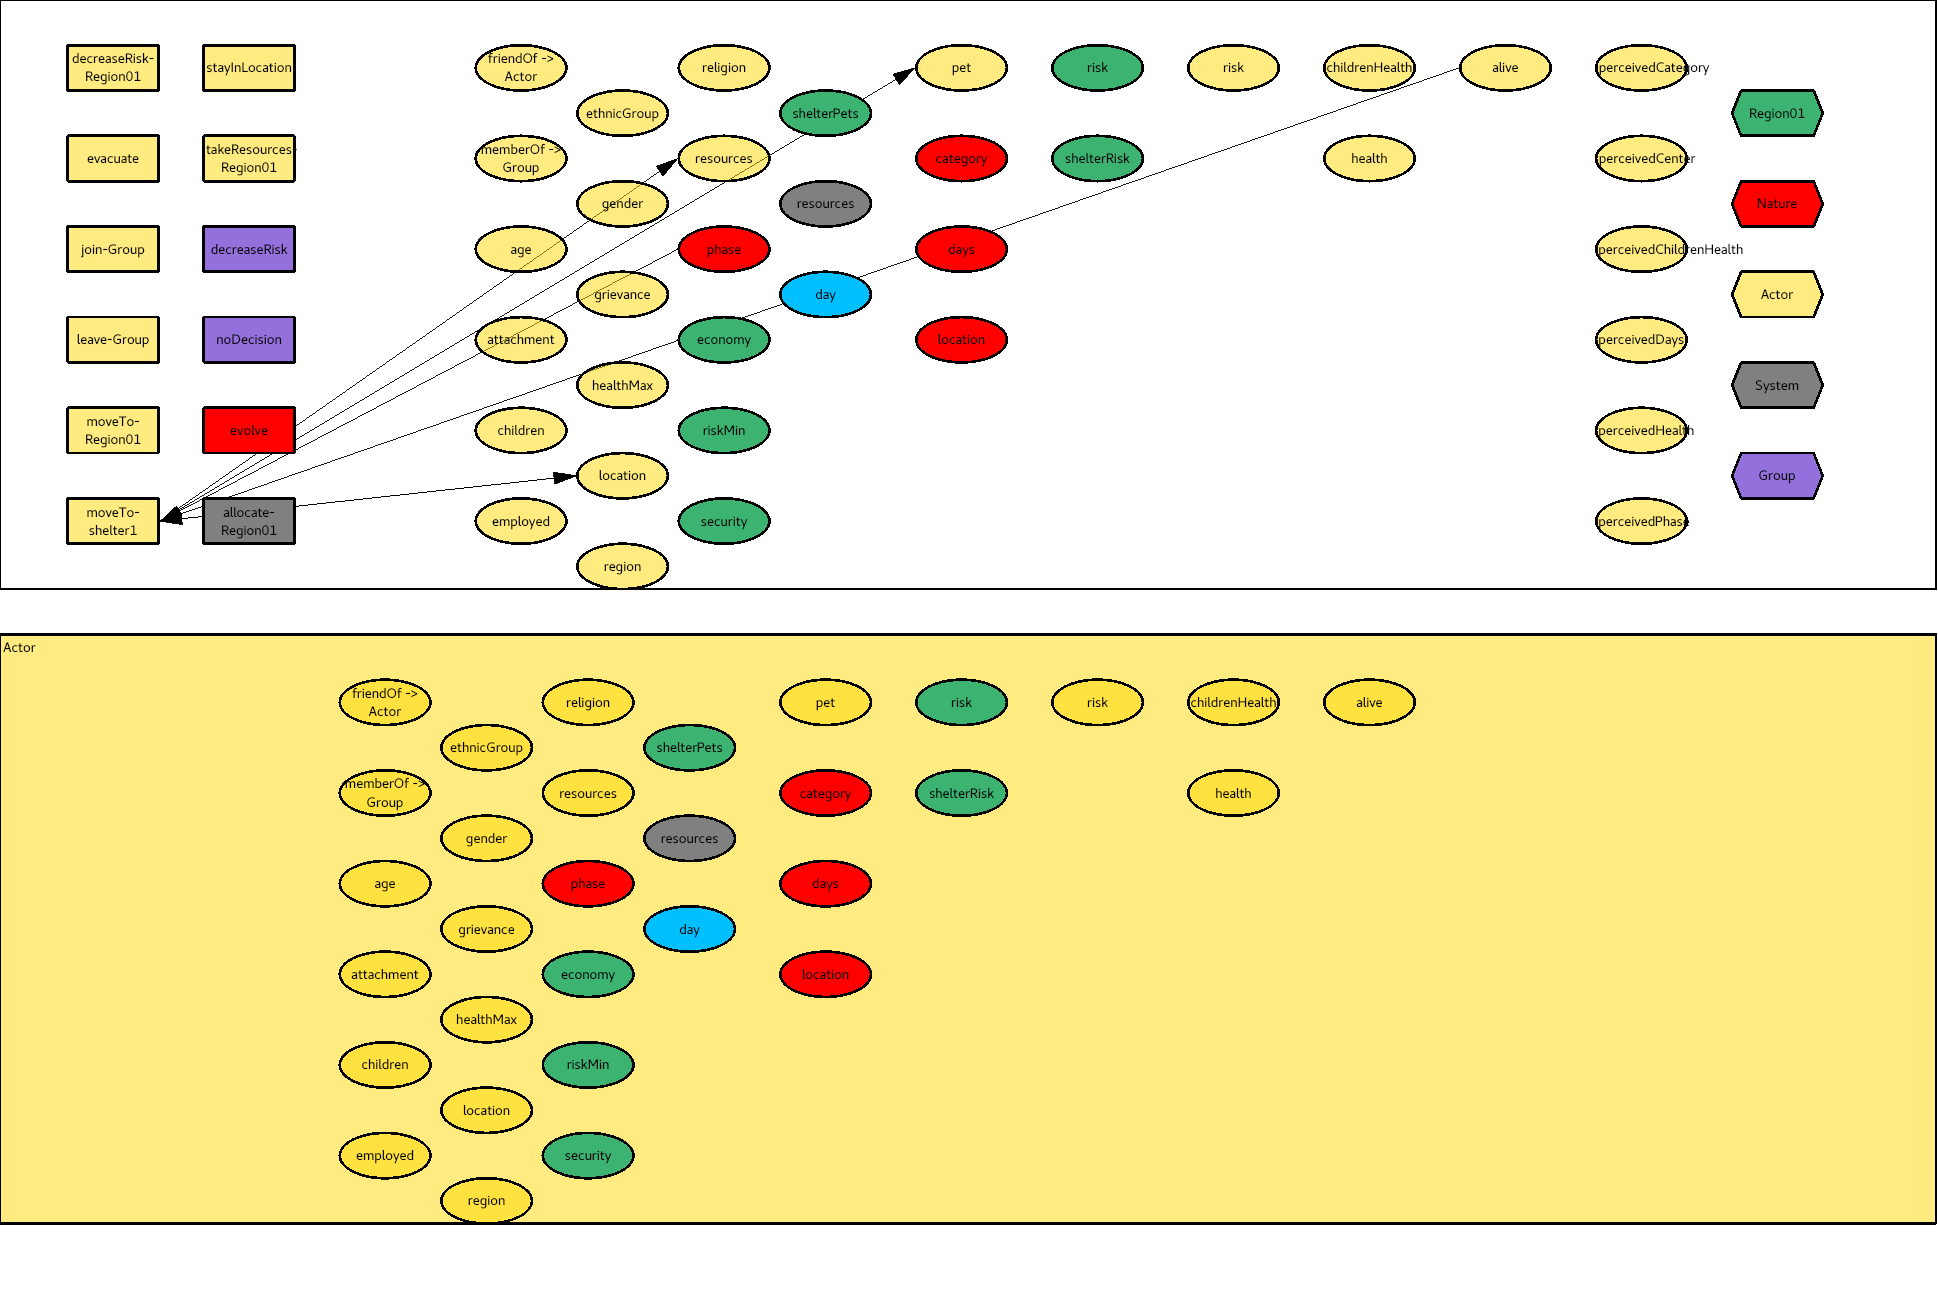
\includegraphics[width=\textwidth]{images/Actor-moveTo-shelter1.png}%
\begin{flushleft}%
\verb|psychsim/domains/groundtruth/simulation/actor.py:317|%
\end{flushleft}%
\subsubsection{Applicability of Actor moveTo shelter1}%
\label{ssubsec:Applicability of Actor moveTo shelter1}%
\begin{flushleft}%
IF %
\textbf{Nature's phase}%
$=$%
\textbf{none}%
\linebreak%
\hspace*{2em}%
THEN %
: %
\textbf{false}%
\linebreak%
\hspace*{2em}%
ELSE %
: %
IF %
\textbf{Actor's alive}%
\linebreak%
\hspace*{4em}%
THEN %
: %
IF %
\textbf{Actor's location}%
$=$%
\textbf{shelter1}%
\linebreak%
\hspace*{6em}%
THEN %
: %
\textbf{false}%
\linebreak%
\hspace*{6em}%
ELSE %
: %
\textbf{true}%
\linebreak%
\hspace*{4em}%
ELSE %
: %
\textbf{false}%
\end{flushleft}

%
\subsubsection{Effect on Actor's location of Actor moveTo shelter1}%
\label{ssubsec:Effect on Actor's location of Actor moveTo shelter1}%
\begin{flushleft}%
$\mbox{\textbf{Actor's location}} '$%
$\leftarrow$%
\textbf{shelter1}%
\end{flushleft}

%
\subsubsection{Effect on Actor's pet of Actor moveTo shelter1}%
\label{ssubsec:Effect on Actor's pet of Actor moveTo shelter1}%
\begin{flushleft}%
IF %
$\mbox{\textbf{Actor's location}} '$%
$=$%
\textbf{shelter1}%
\linebreak%
\hspace*{2em}%
THEN %
: %
IF %
\textbf{Region01's shelterPets}%
\linebreak%
\hspace*{4em}%
THEN %
: %
$\mbox{\textbf{Actor's pet}} '$%
$\leftarrow$%
\textbf{Actor's pet}%
\linebreak%
\hspace*{4em}%
ELSE %
: %
$\mbox{\textbf{Actor's pet}} '$%
$\leftarrow$%
\textbf{false}%
\linebreak%
\hspace*{2em}%
ELSE %
: %
$\mbox{\textbf{Actor's pet}} '$%
$\leftarrow$%
\textbf{Actor's pet}%
\end{flushleft}

%
\subsubsection{Effect on Actor's resources of Actor moveTo shelter1}%
\label{ssubsec:Effect on Actor's resources of Actor moveTo shelter1}%
\begin{flushleft}%
$\mbox{\textbf{Actor's resources}} '$%
$\leftarrow$%
0\%%
$\cdot$%
\textbf{Actor's resources}%
\end{flushleft}

%
\subsection{Actor stayInLocation None}%
\label{subsec:Actor stayInLocation None}%
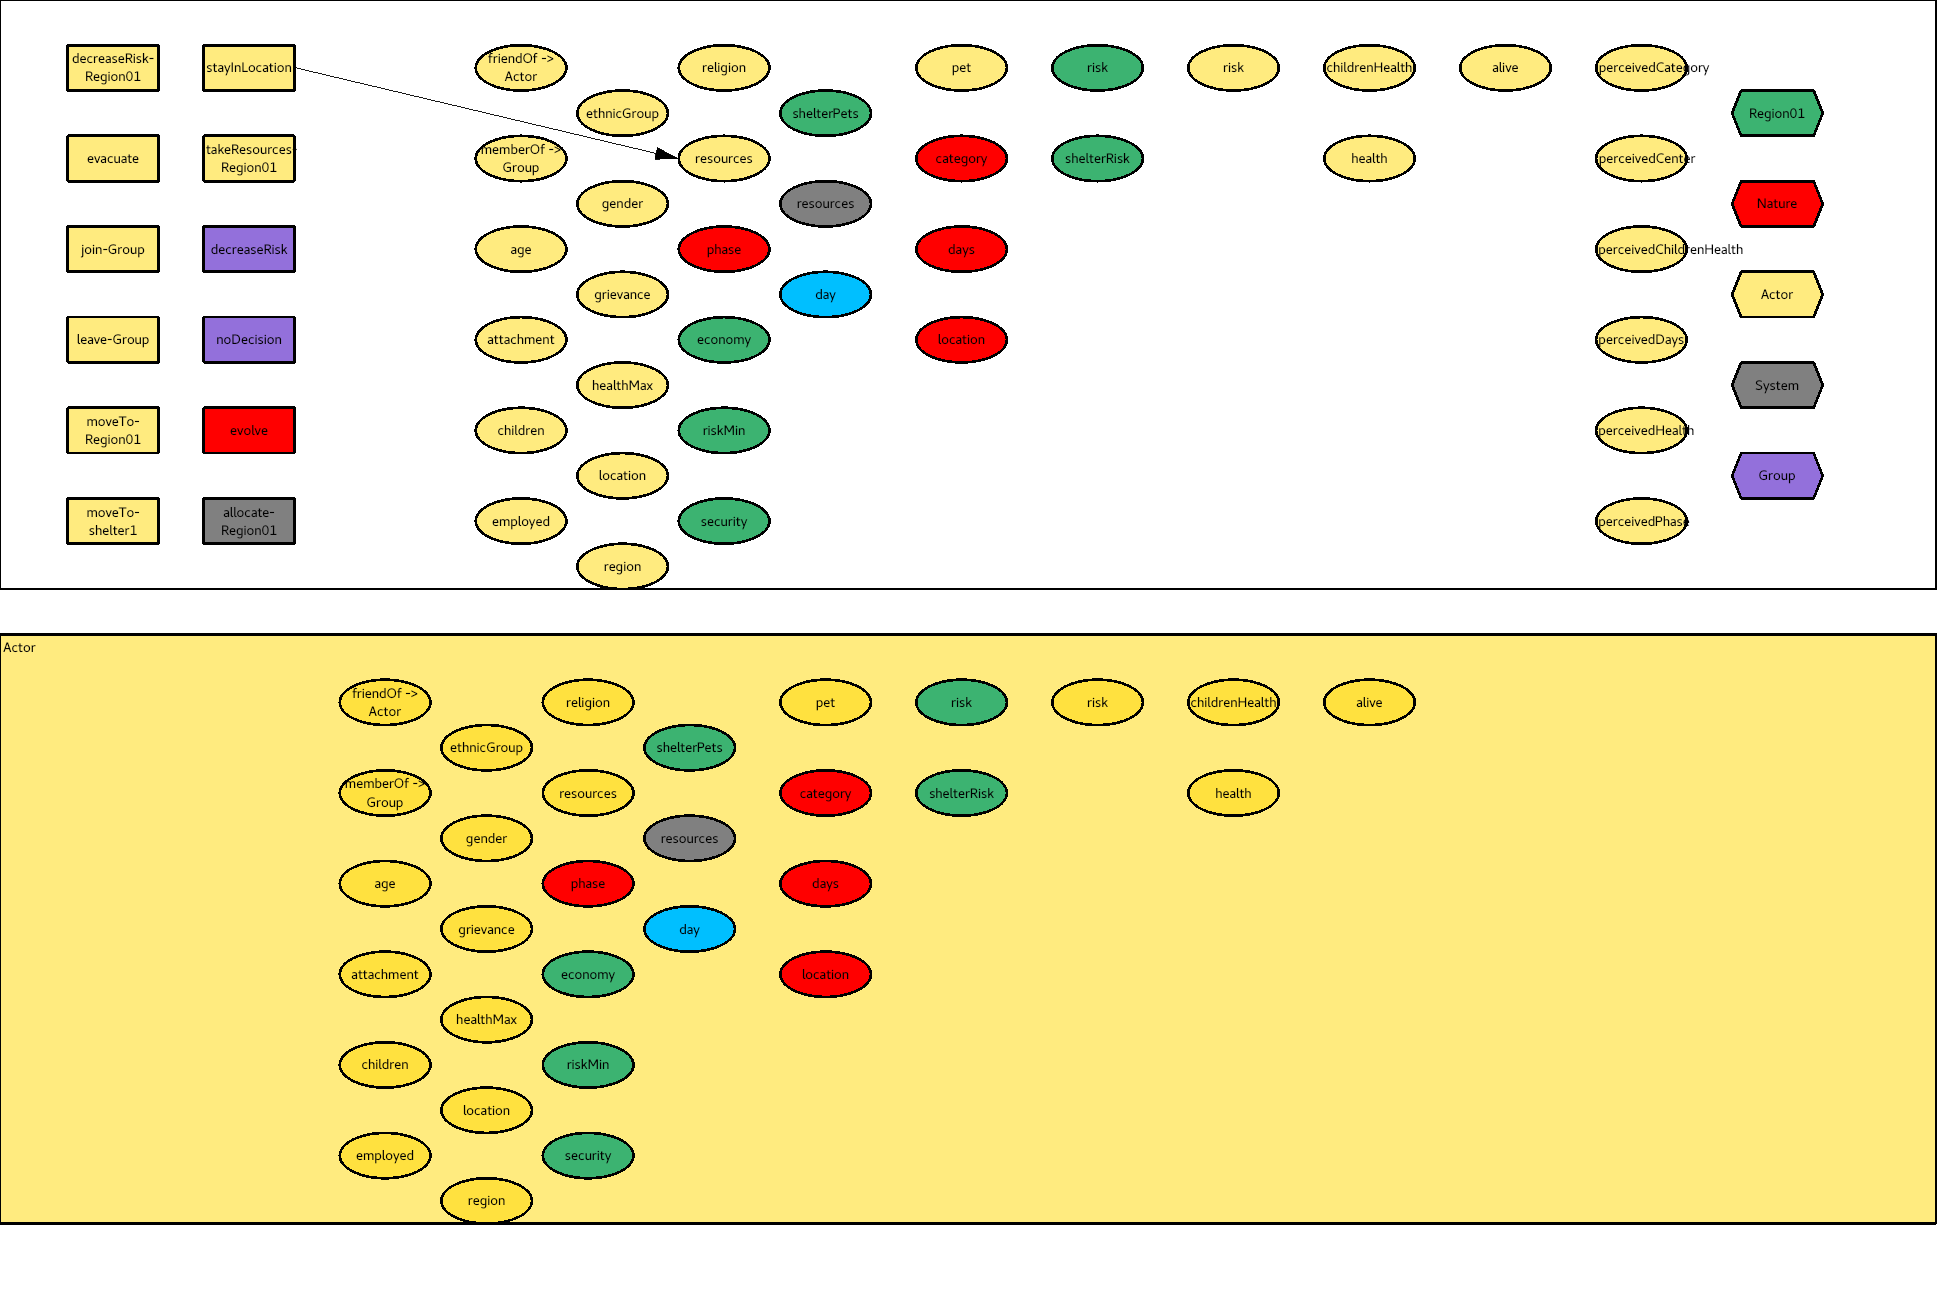
\includegraphics[width=\textwidth]{images/Actor-stayInLocation.png}%
\begin{flushleft}%
\verb|psychsim/domains/groundtruth/simulation/actor.py:277|%
\end{flushleft}%
\subsubsection{Effect on Actor's resources of Actor stayInLocation None}%
\label{ssubsec:Effect on Actor's resources of Actor stayInLocation None}%
\begin{flushleft}%
IF %
\textbf{Actor's alive}%
\linebreak%
\hspace*{2em}%
THEN %
: %
IF %
\textbf{Actor's employed}%
\linebreak%
\hspace*{4em}%
THEN %
: %
IF %
\textbf{Actor's location}%
$=$%
\textbf{\{'Region01', 'evacuated'\}}%
\linebreak%
\hspace*{6em}%
THEN %
: %
$\mbox{\textbf{Actor's resources}} '$%
$\leftarrow$%
60\%%
$\cdot$%
\textbf{Actor's resources}%
+0.40%
\linebreak%
\hspace*{6em}%
ELSE %
: %
$\mbox{\textbf{Actor's resources}} '$%
$\leftarrow$%
\textbf{Actor's resources}%
\linebreak%
\hspace*{4em}%
ELSE %
: %
$\mbox{\textbf{Actor's resources}} '$%
$\leftarrow$%
\textbf{Actor's resources}%
\linebreak%
\hspace*{2em}%
ELSE %
: %
$\mbox{\textbf{Actor's resources}} '$%
$\leftarrow$%
\textbf{Actor's resources}%
\end{flushleft}

%
\subsection{Actor takeResources Region01}%
\label{subsec:Actor takeResources Region01}%
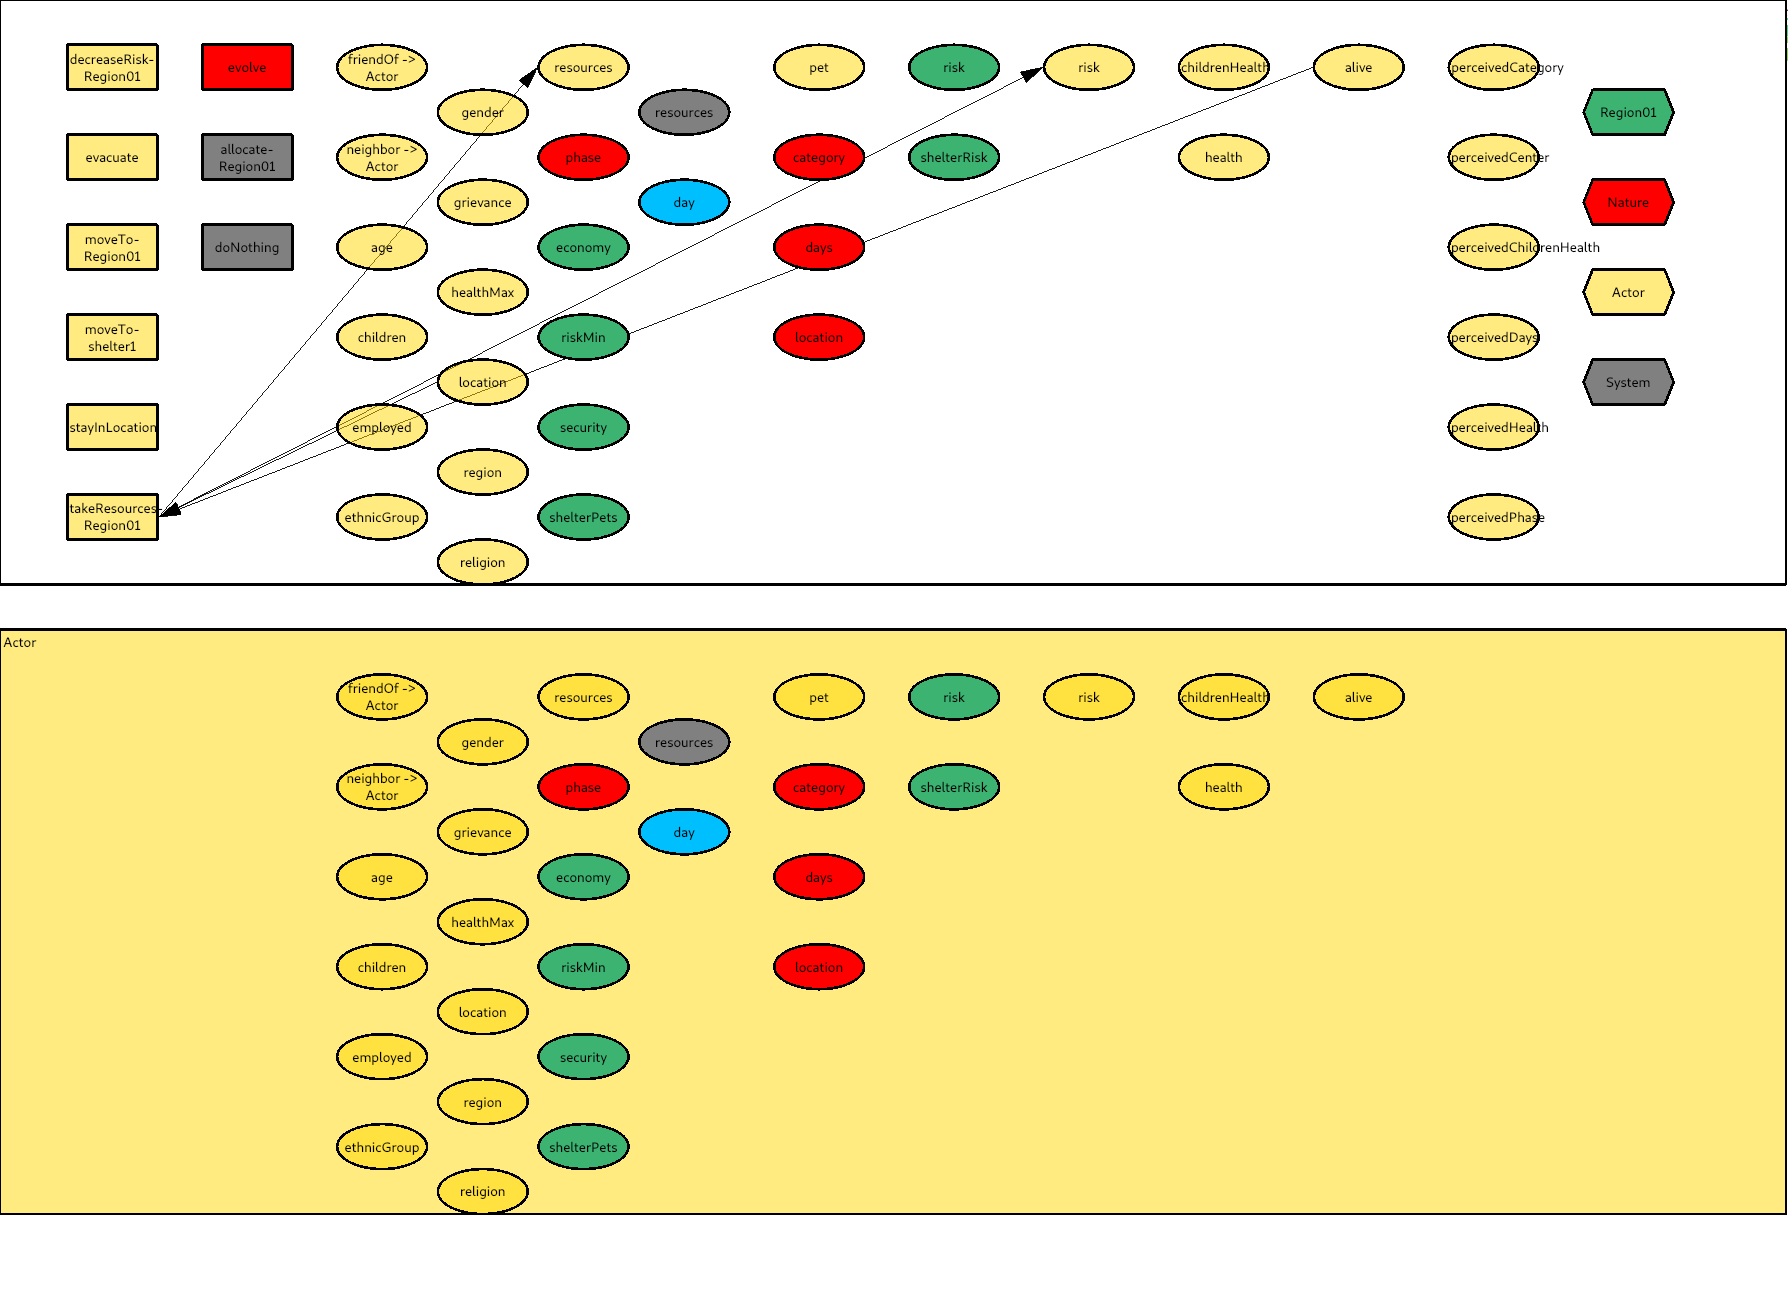
\includegraphics[width=\textwidth]{images/Actor-takeResources-Region01.png}%
\begin{flushleft}%
\verb|psychsim/domains/groundtruth/simulation/actor.py:380|%
\end{flushleft}%
\subsubsection{Applicability of Actor takeResources Region01}%
\label{ssubsec:Applicability of Actor takeResources Region01}%
\begin{flushleft}%
IF %
\textbf{Actor's location}%
$=$%
\textbf{Region01}%
\linebreak%
\hspace*{2em}%
THEN %
: %
IF %
\textbf{Actor's alive}%
\linebreak%
\hspace*{4em}%
THEN %
: %
\textbf{true}%
\linebreak%
\hspace*{4em}%
ELSE %
: %
\textbf{false}%
\linebreak%
\hspace*{2em}%
ELSE %
: %
\textbf{false}%
\end{flushleft}

%
\subsubsection{Effect on Actor's resources of Actor takeResources Region01}%
\label{ssubsec:Effect on Actor's resources of Actor takeResources Region01}%
\begin{flushleft}%
$\mbox{\textbf{Actor's resources}} '$%
$\leftarrow$%
80\%%
$\cdot$%
\textbf{Actor's resources}%
+0.20%
\end{flushleft}

%
\subsubsection{Effect on Actor's risk of Actor takeResources Region01}%
\label{ssubsec:Effect on Actor's risk of Actor takeResources Region01}%
\begin{flushleft}%
IF %
\textbf{Nature's phase}%
$=$%
\textbf{none}%
\linebreak%
\hspace*{2em}%
THEN %
: %
$\mbox{\textbf{Actor's risk}} '$%
$\leftarrow$%
19\%%
$\cdot$%
\textbf{Actor's risk}%
+0.80%
\linebreak%
\hspace*{2em}%
ELSE %
: %
$\mbox{\textbf{Actor's risk}} '$%
$\leftarrow$%
40\%%
$\cdot$%
\textbf{Actor's risk}%
+0.60%
\end{flushleft}

%
\subsection{System allocate Region01}%
\label{subsec:System allocate Region01}%
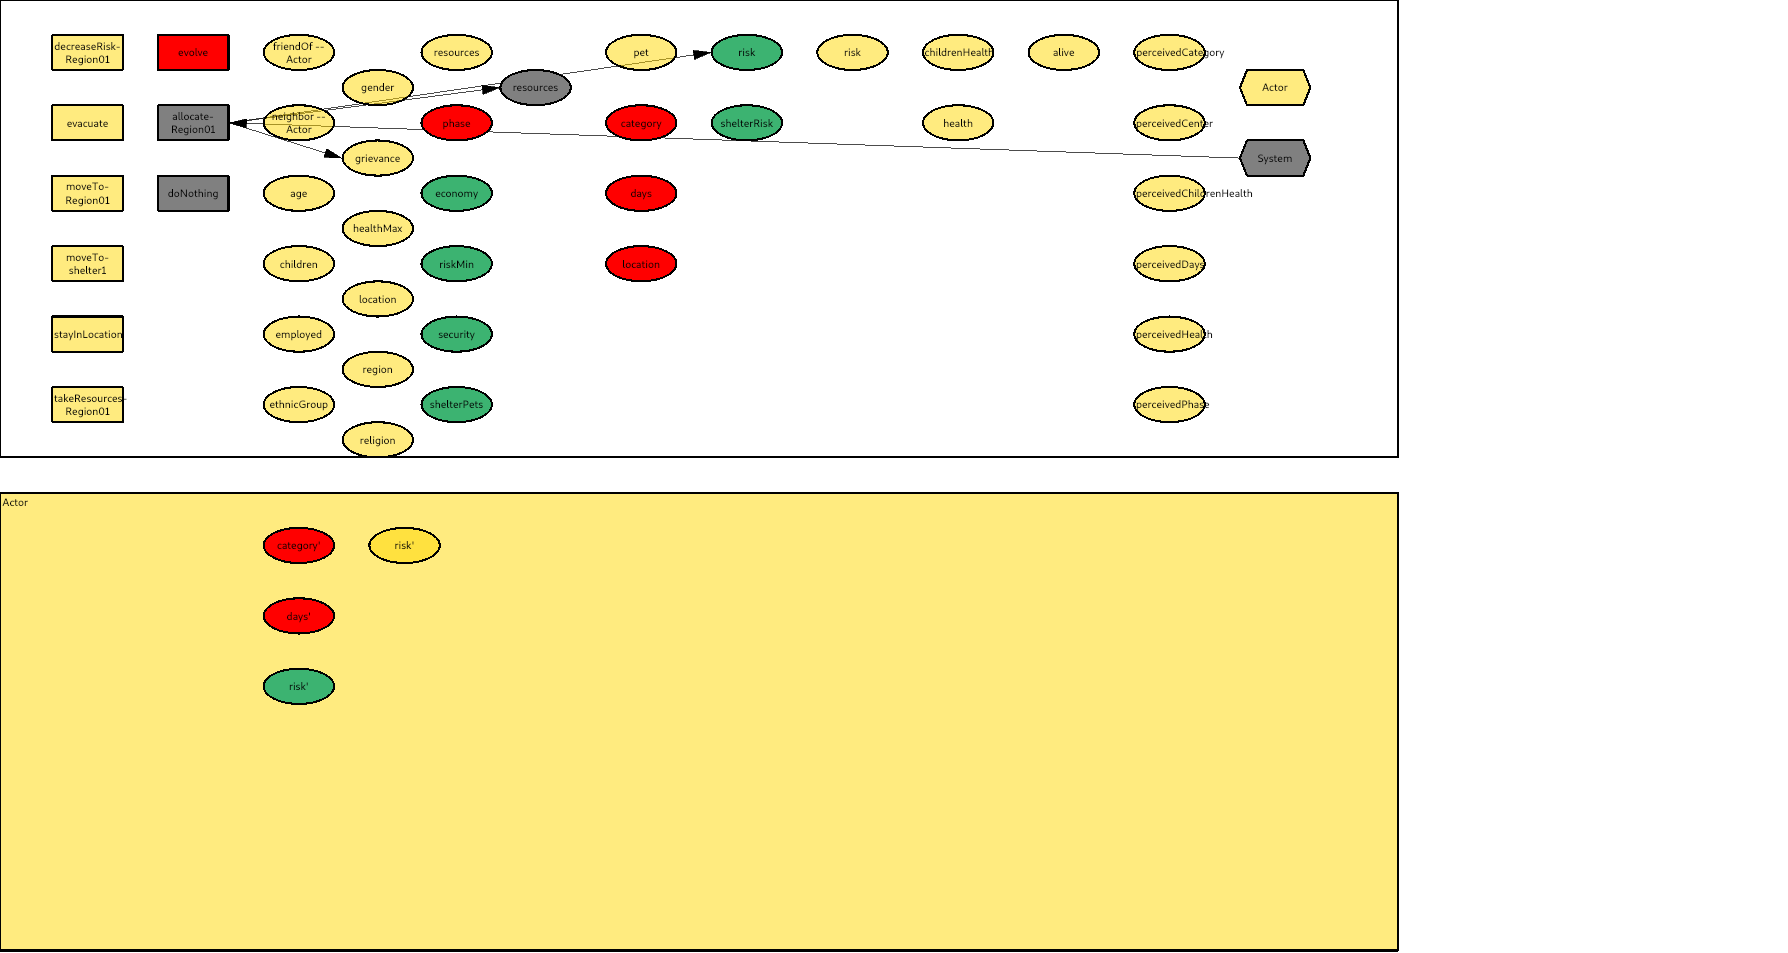
\includegraphics[width=\textwidth]{images/System-allocate-Region01.png}%
\begin{flushleft}%
\verb|psychsim/domains/groundtruth/simulation/system.py:38|%
\end{flushleft}%
\subsubsection{Effect on Actor's grievance of System allocate Region01}%
\label{ssubsec:Effect on Actor's grievance of System allocate Region01}%
\begin{flushleft}%
IF %
\textbf{Actor's region}%
$=$%
\textbf{Region01}%
\linebreak%
\hspace*{2em}%
THEN %
: %
$\mbox{\textbf{Actor's grievance}} '$%
$\leftarrow$%
80\%%
$\cdot$%
\textbf{Actor's grievance}%
\linebreak%
\hspace*{2em}%
ELSE %
: %
$\mbox{\textbf{Actor's grievance}} '$%
$\leftarrow$%
80\%%
$\cdot$%
\textbf{Actor's grievance}%
+0.20%
\end{flushleft}

%
\subsubsection{Effect on Region01's risk of System allocate Region01}%
\label{ssubsec:Effect on Region01's risk of System allocate Region01}%
\begin{flushleft}%
$\mbox{\textbf{Region01's risk}} '$%
$\leftarrow$%
80\%%
$\cdot$%
\textbf{Region01's risk}%
\end{flushleft}

%
\subsubsection{Effect on System's resources of System allocate Region01}%
\label{ssubsec:Effect on System's resources of System allocate Region01}%
\begin{flushleft}%
$\mbox{\textbf{System's resources}} '$%
$\leftarrow$%
\textbf{System's resources}%
\end{flushleft}

%
\subsection{System doNothing None}%
\label{subsec:System doNothing None}%
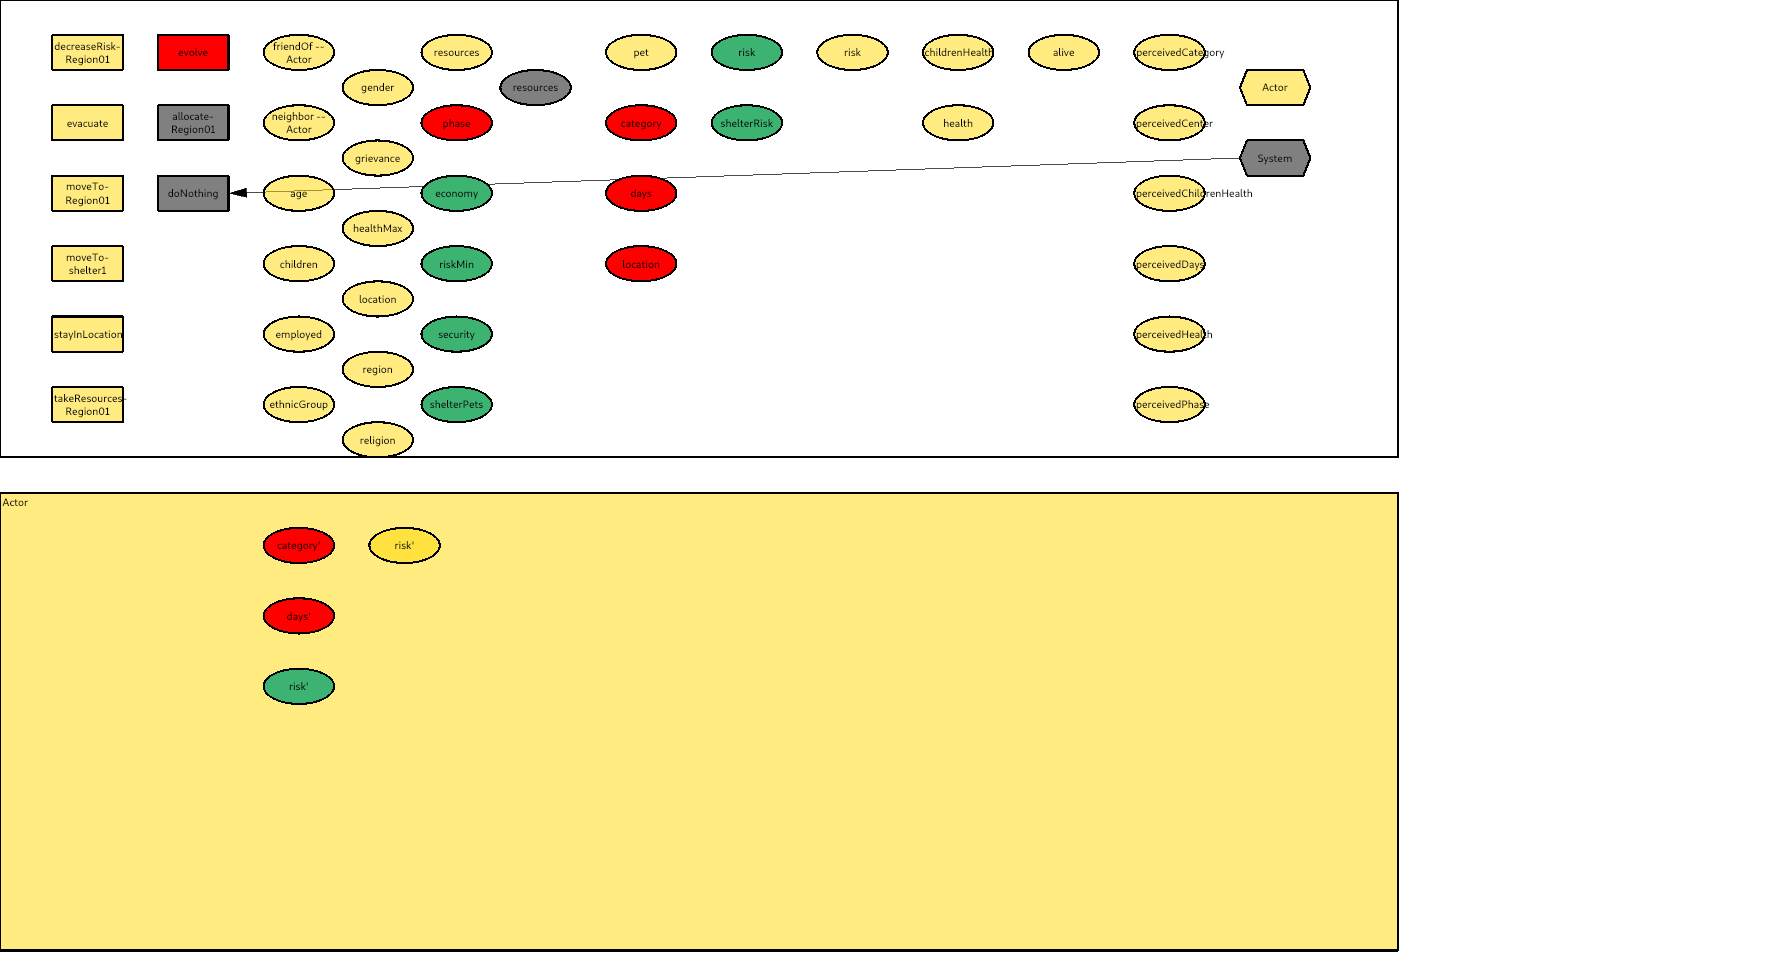
\includegraphics[width=\textwidth]{images/System-doNothing.png}%
\begin{flushleft}%
\verb|psychsim/domains/groundtruth/simulation/system.py:35|%
\end{flushleft}

%
\section{Expected Reward}%
\label{sec:Expected Reward}%
\subsection{Actor's Reward}%
\label{subsec:Actor's Reward}%
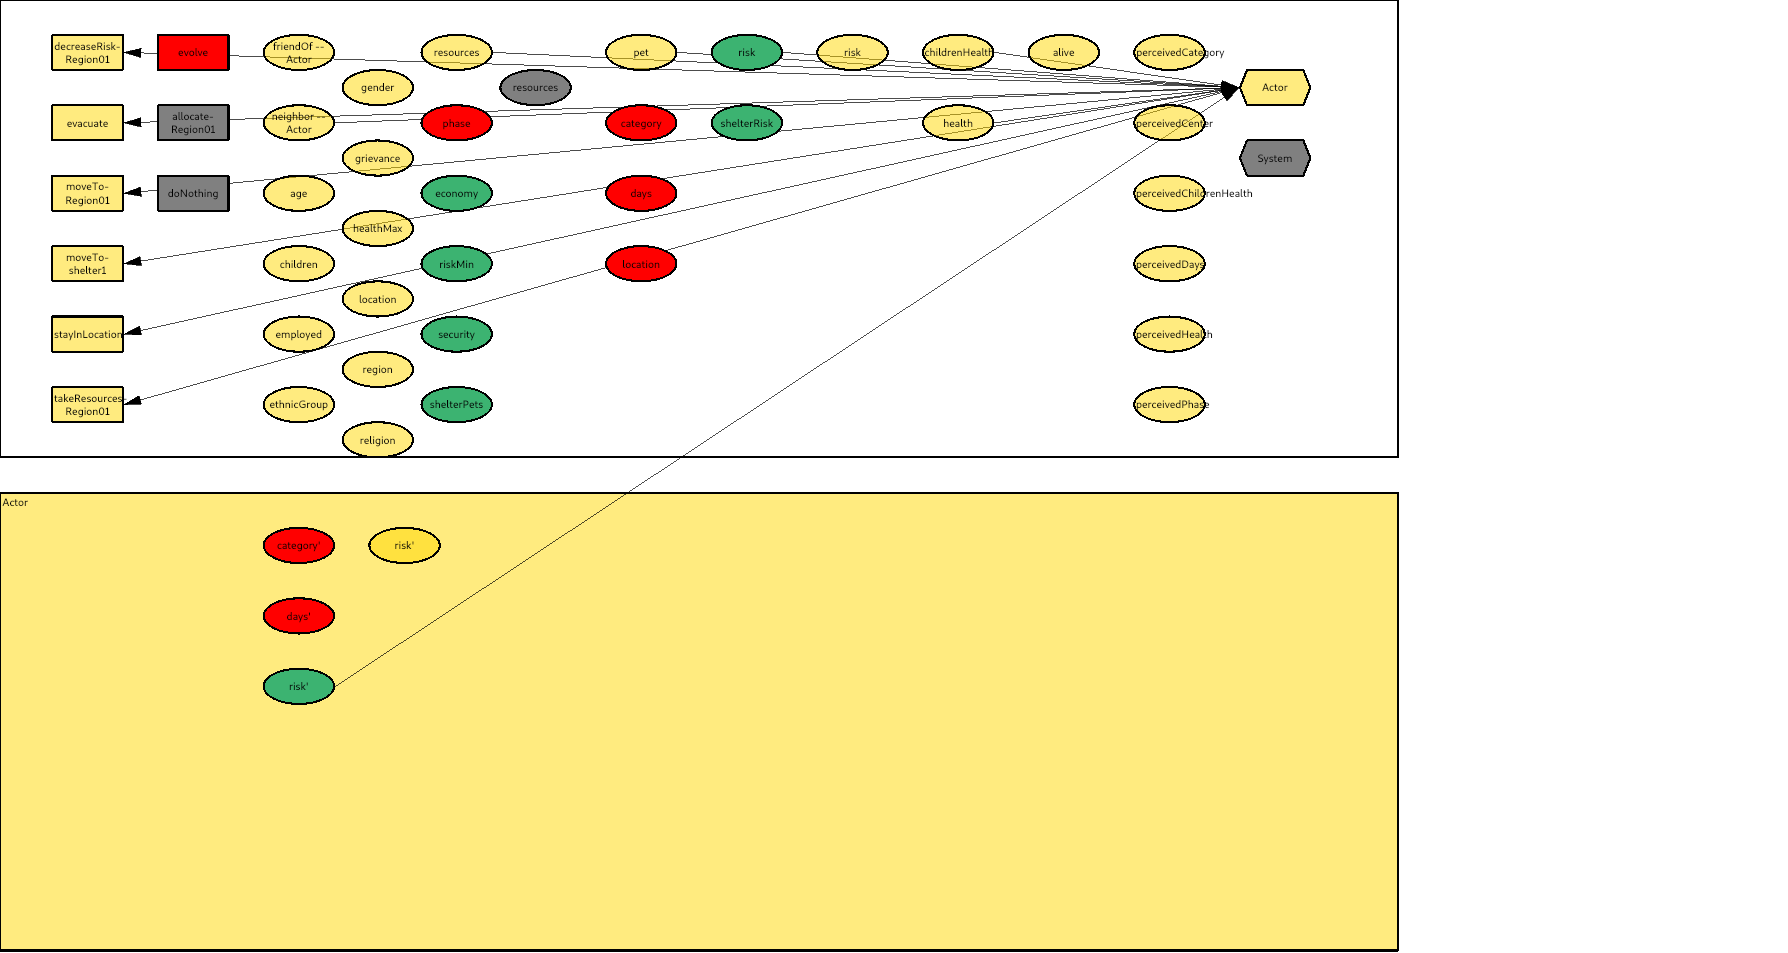
\includegraphics[width=\textwidth]{images/Actor.png}%
\begin{flushleft}%
$R$%
$\leftarrow$%
0\%%
$\cdot$%
\textbf{Actor neighbor Actor}%
+%
20\%%
$\cdot$%
\textbf{Actor's childrenHealth}%
+%
40\%%
$\cdot$%
\textbf{Actor's health}%
+%
40\%%
$\cdot$%
\textbf{Actor's pet}%
+%
20\%%
$\cdot$%
\textbf{Actor's resources}%
+%
{-}80\%%
$\cdot$%
\textbf{Region01's risk}%
\end{flushleft}

%
\subsection{System's Reward}%
\label{subsec:System's Reward}%
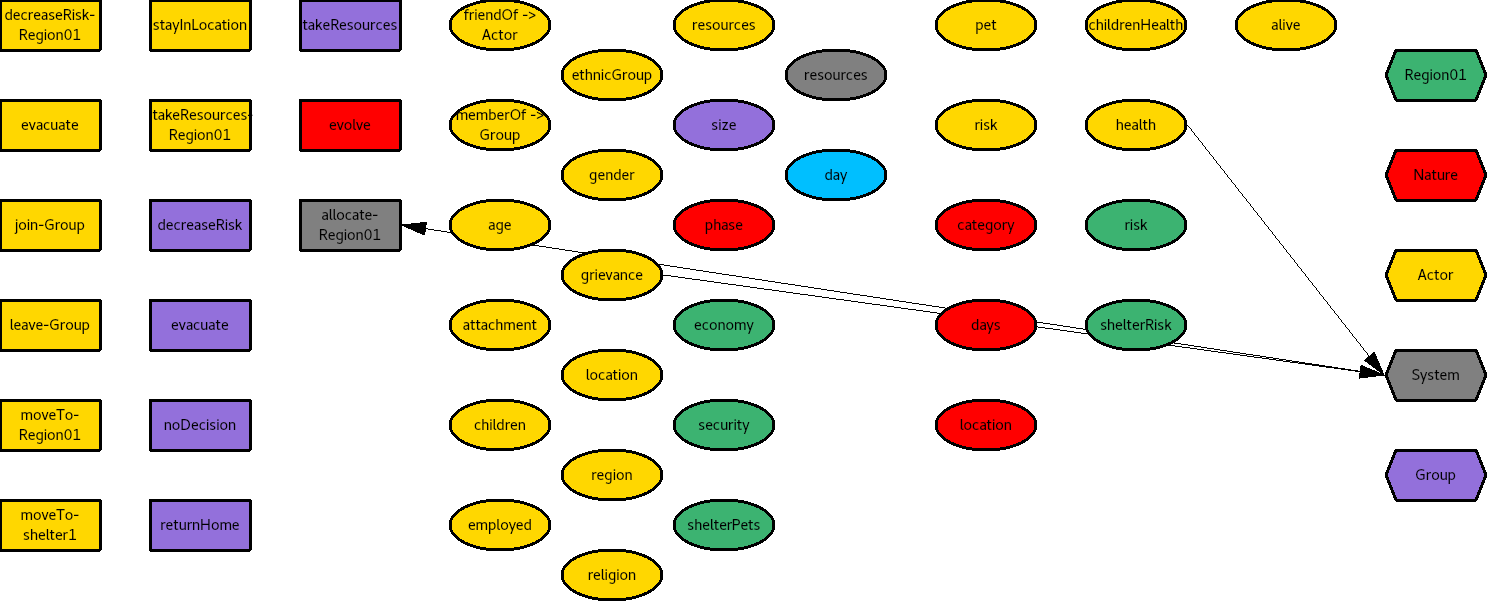
\includegraphics[width=\textwidth]{images/System.png}%
\begin{flushleft}%
$R$%
$\leftarrow$%
{-}20\%%
$\cdot$%
\textbf{Actor's grievance}%
+%
60\%%
$\cdot$%
\textbf{Actor's health}%
\end{flushleft}

%
\end{document}